\chapter{Ergebnisse}
    Innerhalb diese Kapitels geht es zunächst um die Vorbereitung der Proben.
    Weiter geht es es um den Umgang mit dem dreidimensionalen Datensatz sowie dessen Bearbeitung.
    Die verschiedenen extrahierten Darstellungen werden dann aufgenommen und analysiert.
    In dieser Arbeit untersuchten Gold und Nickeloxid Proben wurden alle in dem Versuchsaufbau aus \autoref{sec:Versuchsaufbau} vorbereitet und vermessen.
    Die Eisenoxid Proben wurden an der NanoESCA Beamline am Synchrotron Elettra in Triest präperiert und charakterisiert \footnote{Näheres zu diesem Versuchsaufbau und der Behandlung der Daten kann in \cite{ma-DJ} gefunden werden.}.

    \section{Gold}
        \begin{figure}
            \centering
            \begin{subfigure}{0.48\textwidth}
                \centering
                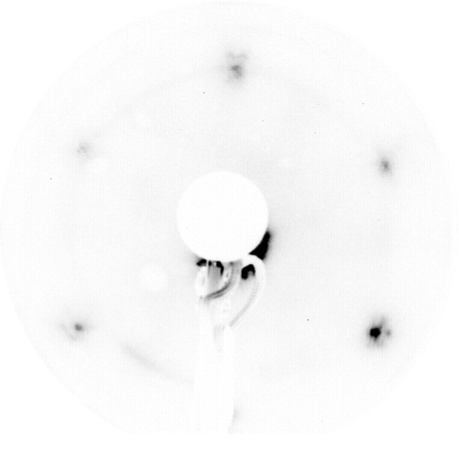
\includegraphics[height=5cm]{./content/pictures/Au/2021_06_08_002_Au(111)_75eV}
                \subcaption{Gold (111) bei einer Elektronenenergie von \SI{75}{\electronvolt}.}
                \label{fig:LEED_Au}
            \end{subfigure}
            \begin{subfigure}{0.48\textwidth}
                \centering
                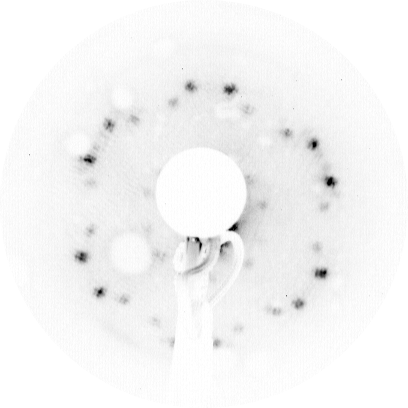
\includegraphics[height=5cm]{./content/pictures/Au+5A/021_Au(111)+5A(40)_16eV.png}
                \subcaption{Eine Monolage Pentacene auf dem sauberen Gold bei einer Energie von \SI{16}{\electronvolt}.}
                \label{fig:LEED_Au+5A}
            \end{subfigure}
            \caption{Die LEED-Bilder für die Kalibrierung des Pentacene.}
        \label{fig:Substrate}
        \end{figure}
        Zunächst geht es hier um das Substrat auf dem später der antiferromagnetische Nickeloxidfilm gewachsen wird.
        Das Substrat wurde zunächste mehrer Male durch ioneninduziertes Zerstäuben und anschließendes Aufheizen auf \SI{500}{\celsius} gereinigt.
        Es ergibt sich eine wohldefinierte Struktur der Oberfläche, was sich ebenfalls in dem Beugungsbild der niederenergetischen Elektronen in \autoref{fig:LEED_Au} erkennen lässt.
        Ferner sind scharfe Spots zu erkennen, ebenso wie die charakteristische kleineren Spots um die Hauptspots, die von der Fischgräten-Rekonstruktion herrühren.
        Die unterschiedlichen Intensität der einzelnen Reflexe rühr ebenfalls von der Rekonstruktion her.

        \begin{figure}
            \centering
            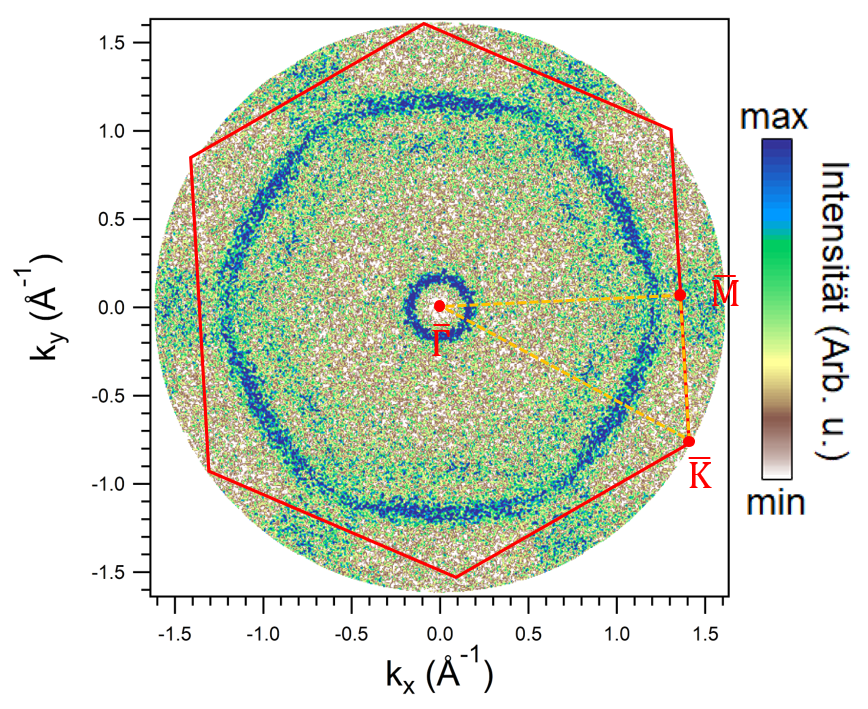
\includegraphics[width=0.5\textwidth]{./content/pictures/Au/BZ_Au.png}
            \caption{Die gemessene Winkelverteilung von Gold (111) an der Fermifläche.
            Eingezeichnet in rot ist die erste Brillouinzone und drei Hochsymmetriepunkte, entlang deren Richtung der Stack für die Bandstruktur geschnitten wird.}
            \label{fig:BZ_Au}
        \end{figure}
        \begin{figure}
            \centering
            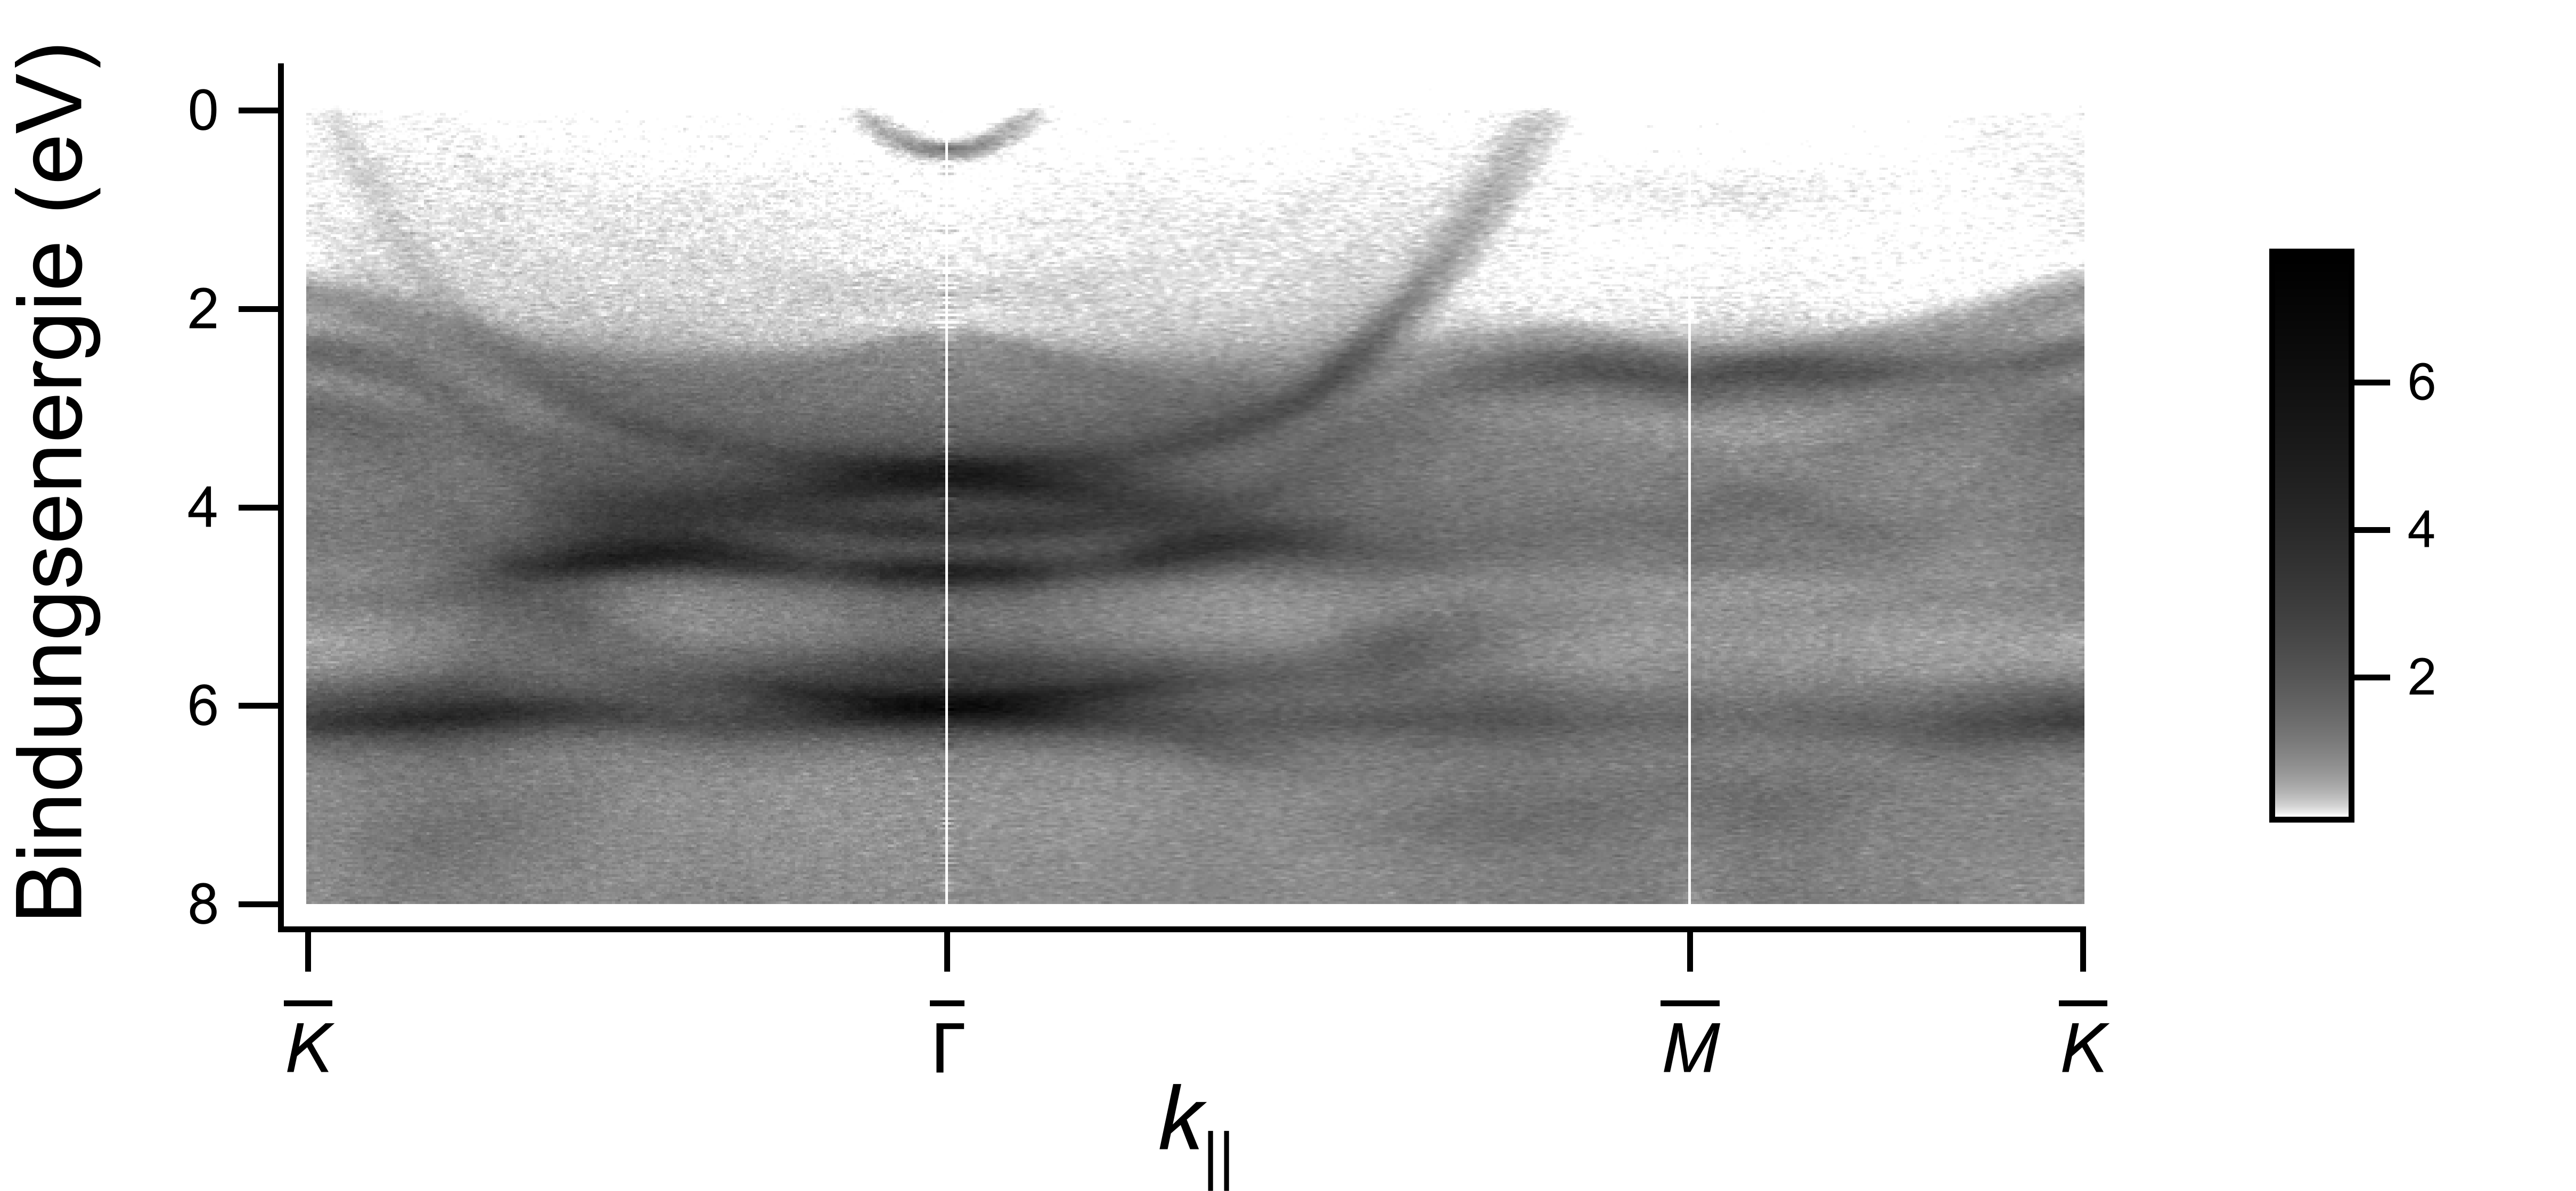
\includegraphics[width=0.8\textwidth]{./content/pictures/Au/Band_Au111.png}
            \caption{Die gemessene Bandstruktur von Gold (111).}
            \label{fig:Band_Au}
        \end{figure}
        Die Eigenschaft, dass Gold einen Oberflächenzustand besitzt ist nützlich um festzustellen ob es sich um eine gut präperierte Oberfläche handelt.
        Der Oberflächenzustand lässt sich in \autoref{fig:BZ_Au} klar erkennen.
        Zusätzlich ist die erste Brillouinzone eingetragen sowie einige Hochsymmetriepunkte.
        Durch Schneiden entlang der Linien zwischen den Hochsymmetriepunkten ergibt sich die Bandstruktur, welche in \autoref{fig:Band_Au} dargestellt ist.
        Die Bindungsenergie wurde ermittelt in dem die Photonenenergie von \SI{21.22}{\electronvolt} angenommen wurde und die Fermikante des Goldes bei \SI{16.55}{\electronvolt} in einem winkelintegrierten Spektrum gefittet wurde.
        Damit wird die Austrittsarbeit des Analysators zu \SI{4.72}{electronvolt} bestimmt, nur dies fließt dann noch in die Gleichung \ref{eqn:Photoeffekt} ein.
        Wird die gesamte Länge des Spektrums betrachtet, also der Energieunterschied zwischen Fermikante und Ende des Sekundärelektronen, so lässt sich die Austrittsarbeit der Probe bestimmen.
        Für Gold lässt sich die Austrittsarbeit auf \SI{5.46}{\electronvolt} ermitteln, was in der selben Ornung wie Literaturwerte liegt~\cite{Hüfner}.

        \begin{figure}
            \centering
            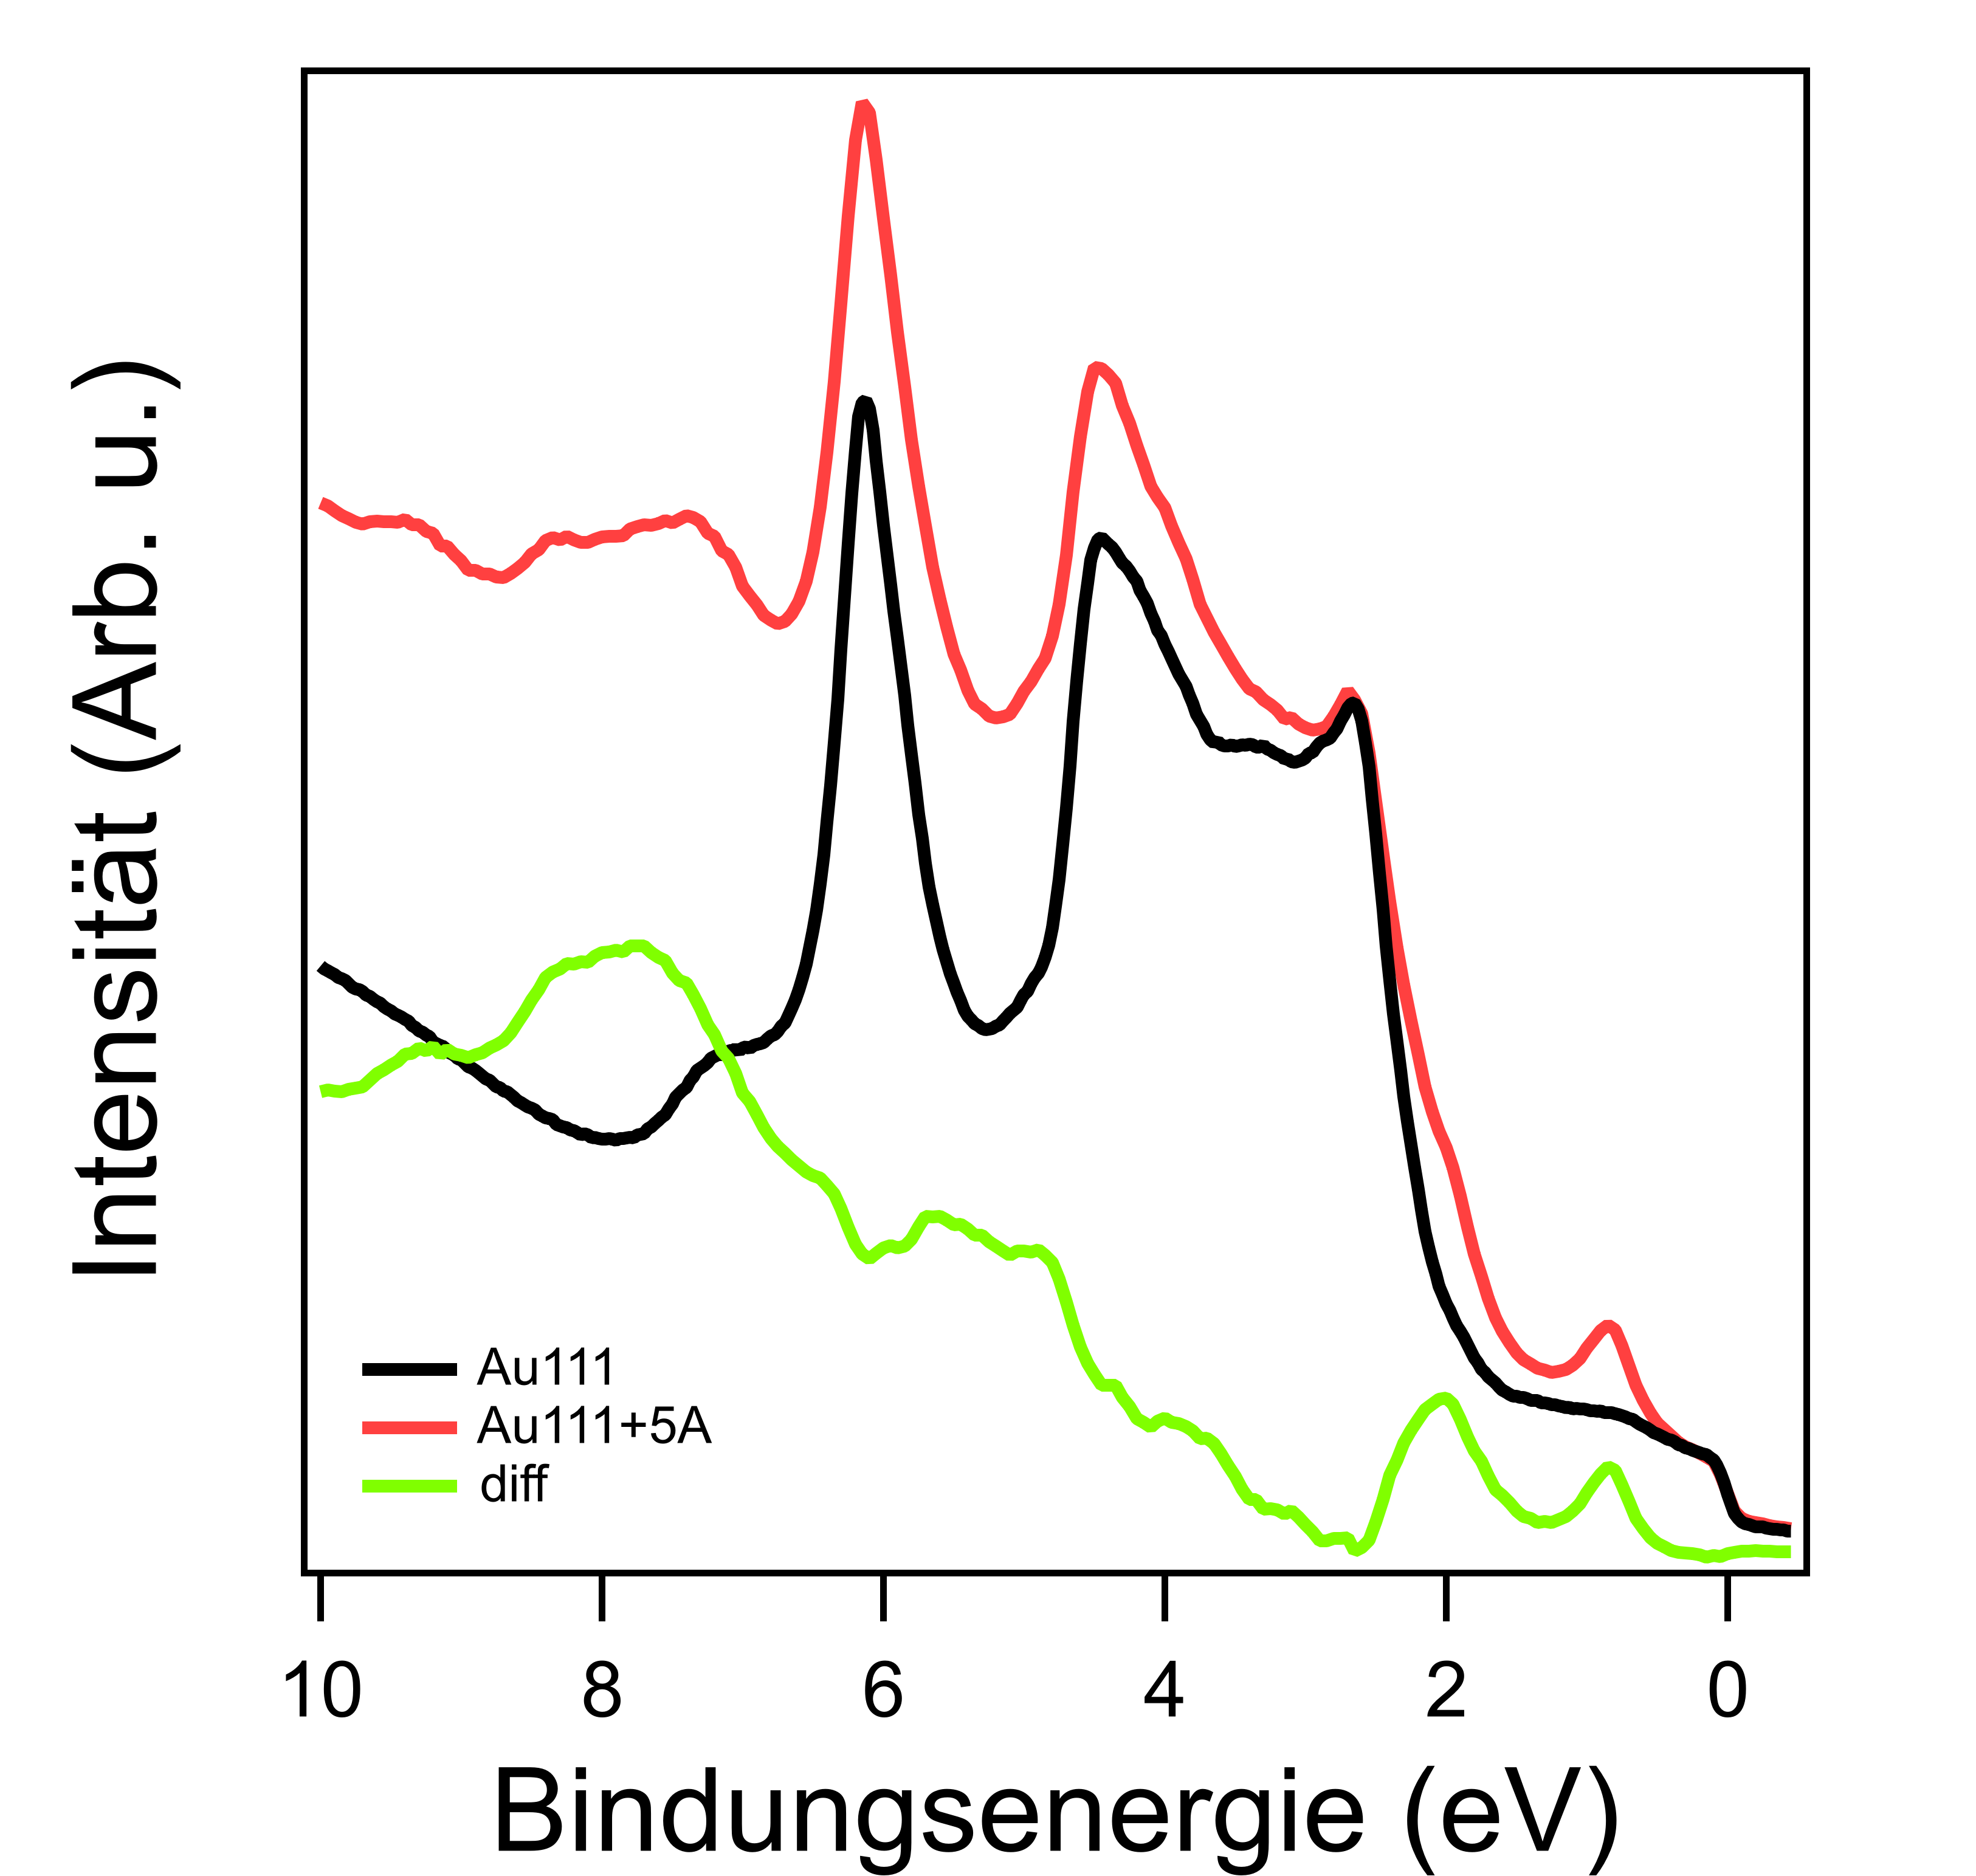
\includegraphics[width=0.5\textwidth]{./content/pictures/Au+5A/EDC_Au_5A.png}
            \caption{Die integrierten Spektren für reines Gold, Gold mit einer Monolage Pentacene und deren Differenz.}
            \label{fig:EDC_Au+5A}
        \end{figure}
        Das Goldsubstrat eignet sich ebenfalls zur Kalibrierung der Monolage von Pentacene, da bereits bekannt ist, dass sich diese flach auf der Oberfläche ordnet \cite{5A_1}.
        Bei der Wechselwirkung mit dem Substrat handelt es sich um die Physisorption durch einen Substrat-Molekülabstand von \SI{3.28}{\angstrom} \cite{5A_1}.
        % Es ergibt sich so das LEED-Bild in \autoref{fig:LEED_Au+5A}, was auch die bekannte \textbf{Überstruktur} (5A_1, 5A_5) aufweist.
        Schaut man sich das winkelintegrierte Spektrum im Bereich der Valenzzustände in \autoref{fig:EDC_Au+5A} an, so sind auch deutlich Elemente zu erkennen, die durch die Molekühle hervorgerufen werden.

        \begin{figure}
            \centering
            \begin{subfigure}[t]{0.48\textwidth}
                \centering
                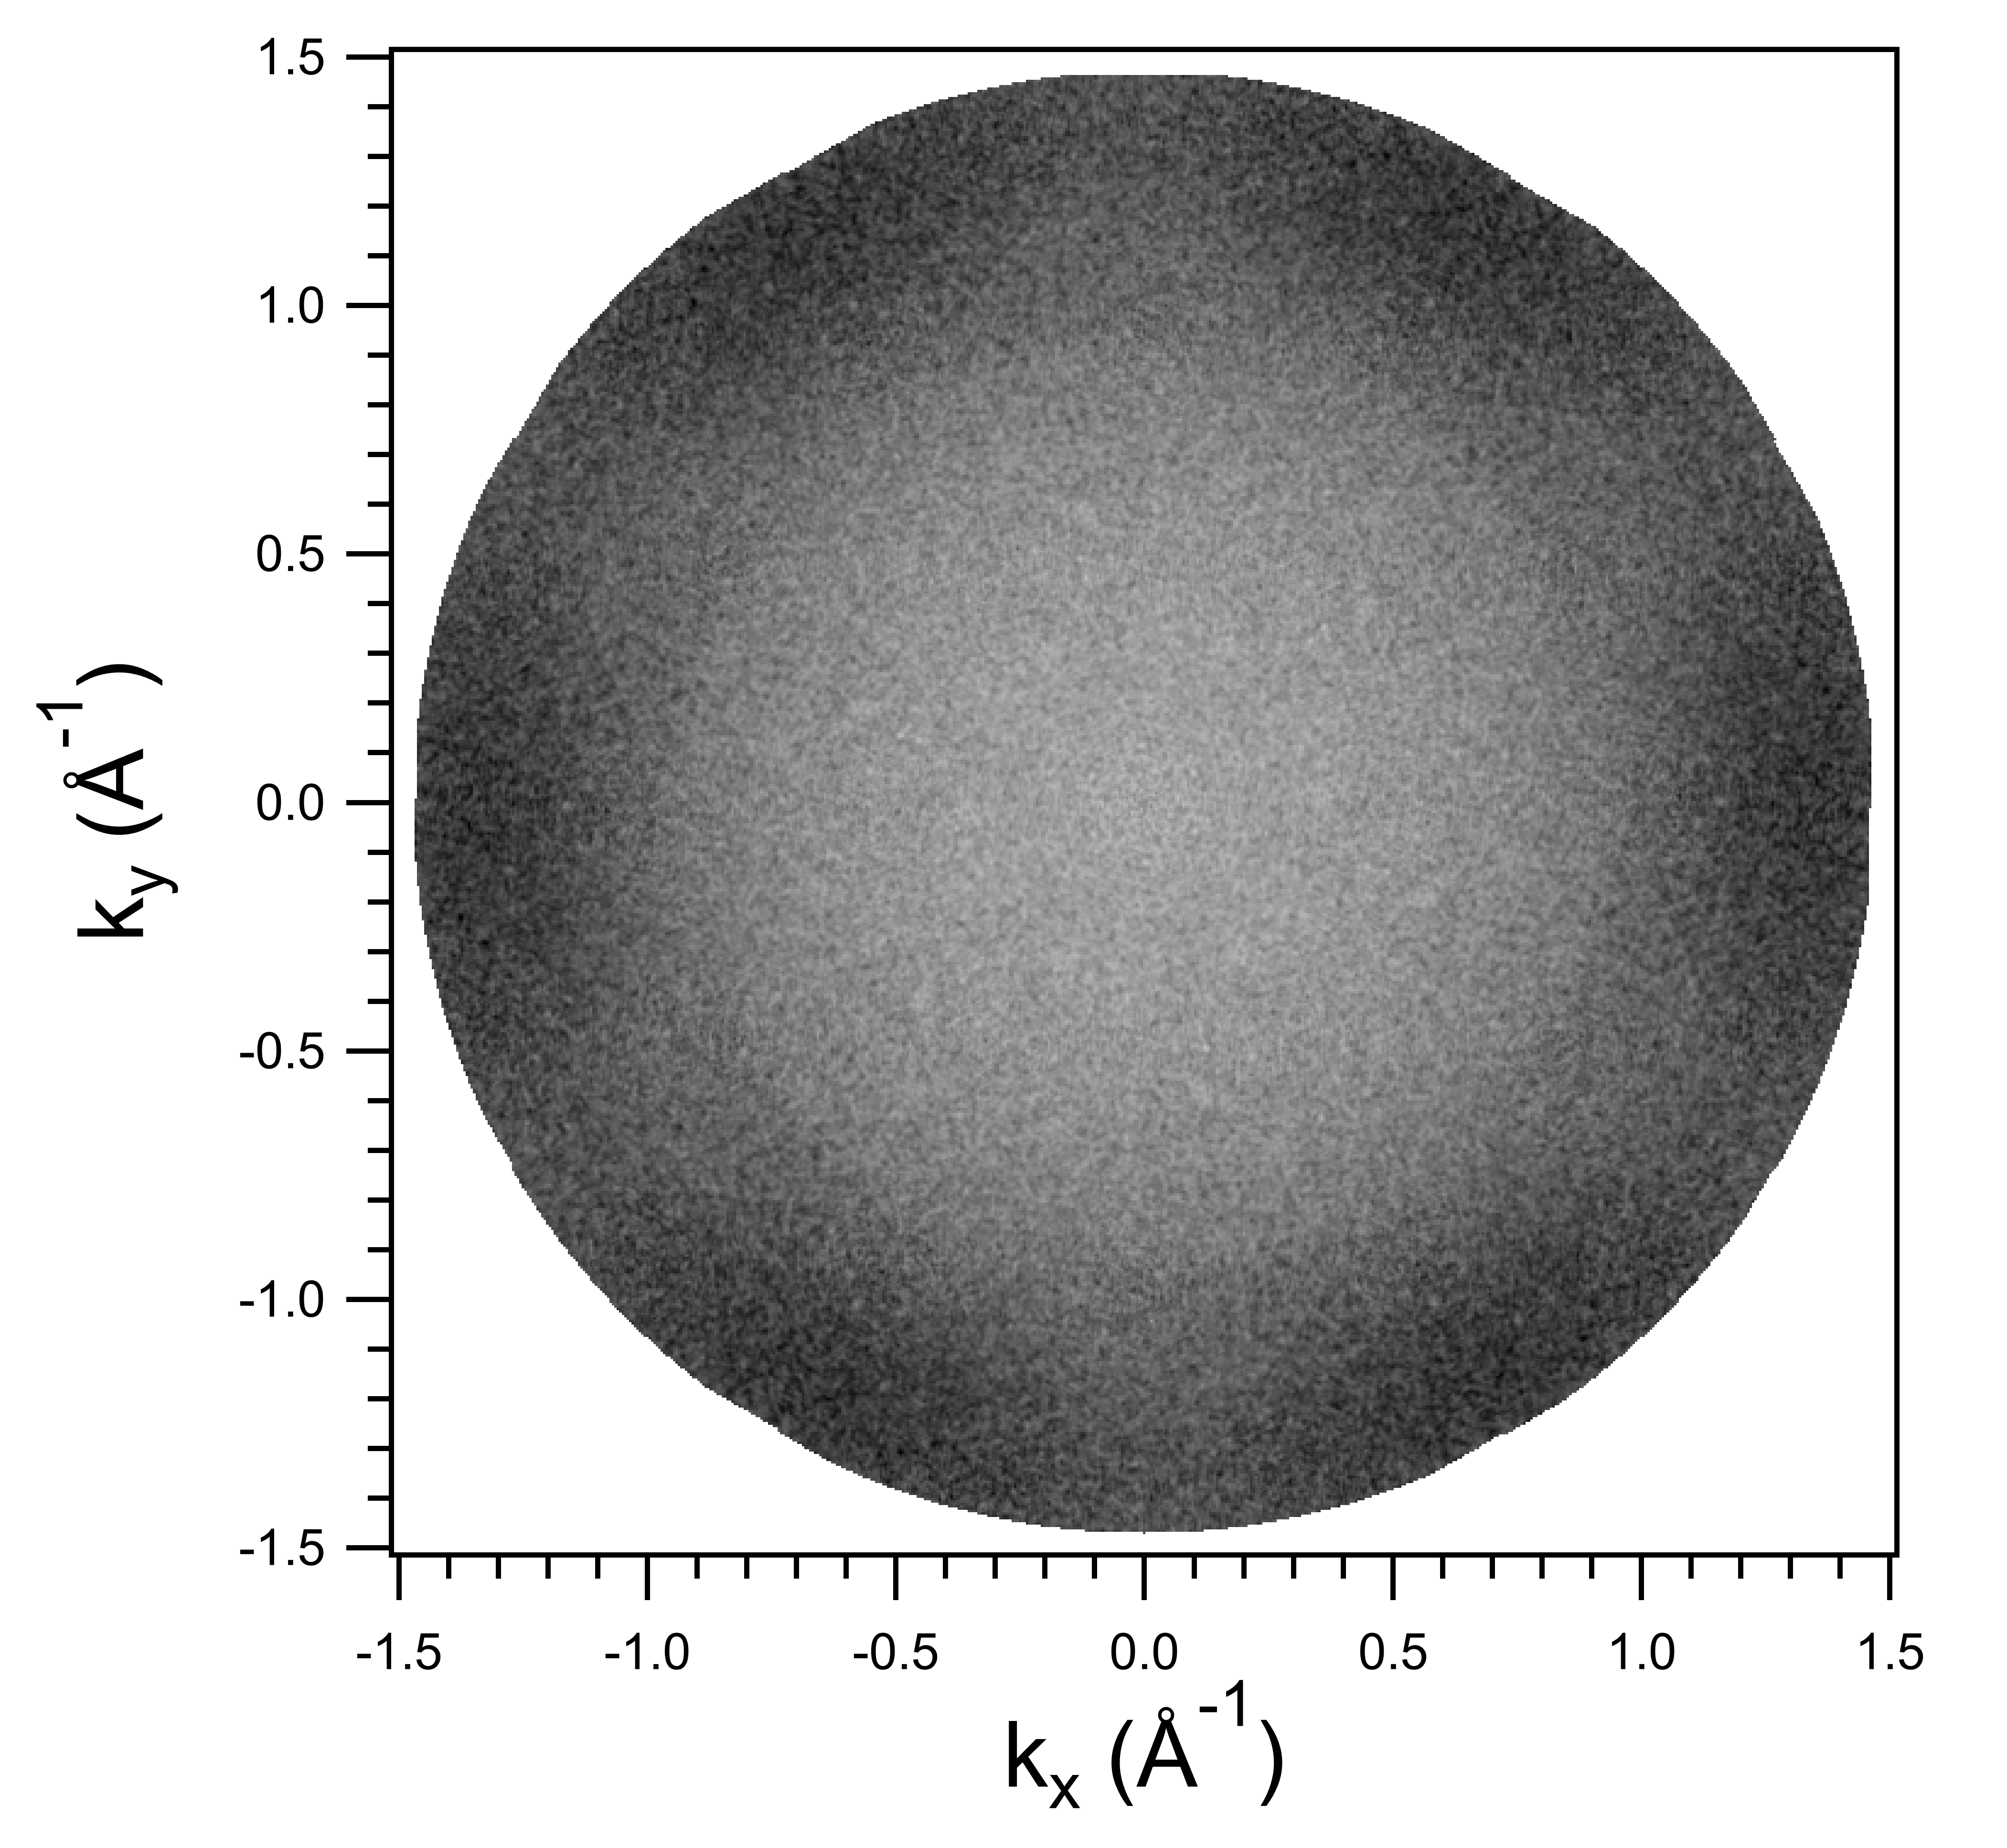
\includegraphics[height=5cm]{./content/pictures/Au+5A/IMAGE_2021_06_17_005_BE0_8}
                \subcaption{Gemmesen, symmetrisiertes Bild bei einer Bindungsenergie von \SI{0.8}{\electronvolt}.}
                \label{fig:MOT_Au+5A_exp}
            \end{subfigure}
            \begin{subfigure}[t]{0.48\textwidth}
                \centering
                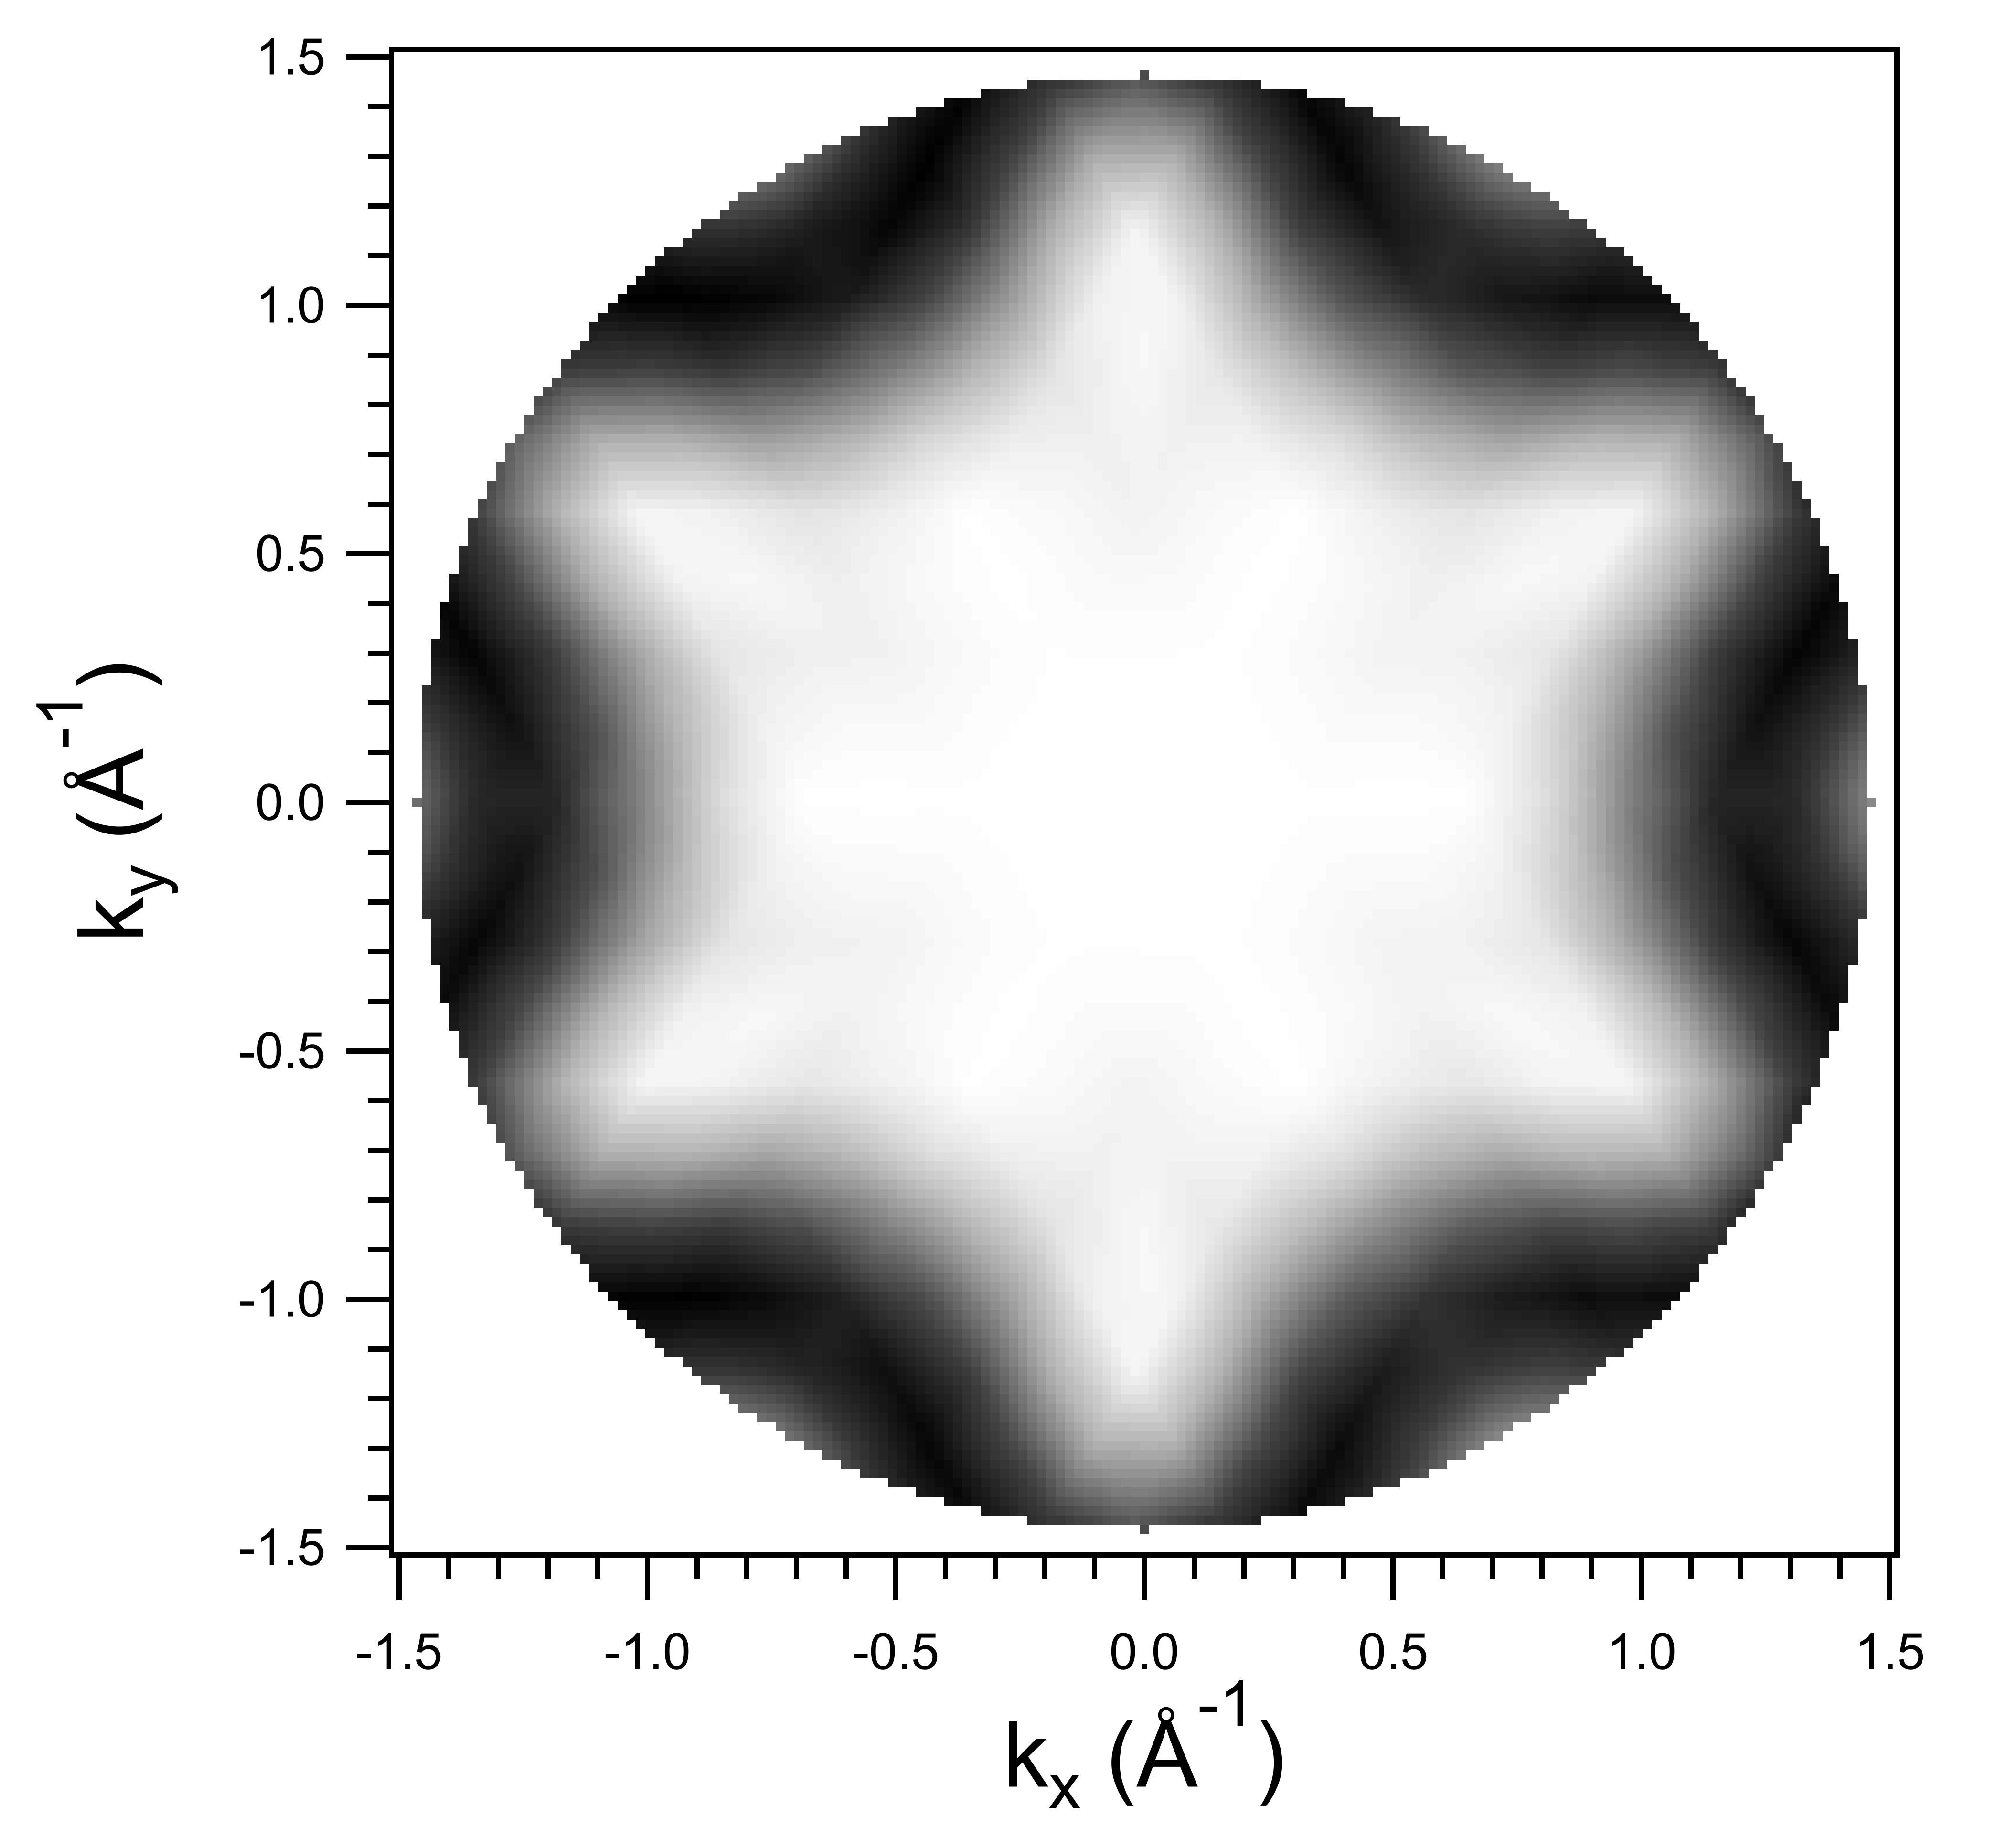
\includegraphics[height=5cm]{./content/pictures/Au+5A/HOMO1_all_CT}
                \subcaption{Theorie Oribtale mit Symmetrisierung zweimal um 120 Grad gedreht und zum Ursprungsbild addiert.}
                \label{fig:MOT_Au+5A_theo}
            \end{subfigure}
            \caption{Zuordnung eines Bildes zu einem der Molekülorbitale.}
            \label{fig:MOT_Au+5A}
        \end{figure}
        Winkelaufgelöste Bilder bei den entsprechenden Energien zeigen auch zusätzliche Merkmale im Bezug zum reinen Gold.
        Gemeinsam mit theoretischen Berechnungen aus der Dichtefunktionaltheorie lassen sich diese dann entsprechenden Molekülorbitalen zuordnen.
        Dies ist für einige Energien und Orbitale in \autoref{fig:MOT_Au+5A} geschehen.
        Dabei wurden die gemessenen wie auch berechneten Bilder entsprechend der Geometrie aus dem Beugungsbild \autoref{fig:LEED_Au+5A} jeweils um \SI{120}{\degree} gedreht und aufsummiert.
        Die theoretisch berechneten Bilder wurden mit Hilfe des Python Programms \textit{kmap.py} erstellt~\cite{brandstetter_kmappy_2021}.
        \begin{itemize}
            \item Peaks der Moleküle kennzeichnen
            \item Alle Molekülorbital zuordnungen vereinigen und ergänzen
            \item Bandstruktur deuten von Gold, Bänder zuordnen?
        \end{itemize}

        
    \section{Nickeloxid}    
        \begin{figure}
            \centering
            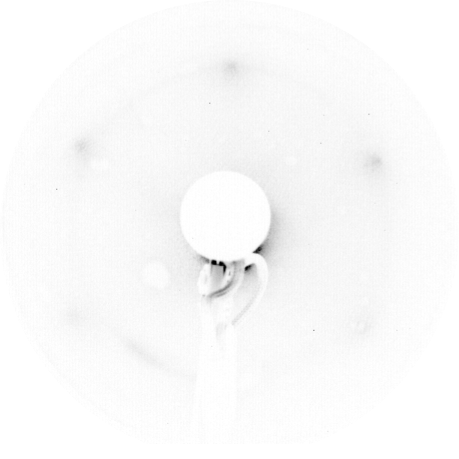
\includegraphics[height=5cm]{./content/pictures/NiO/2021_06_15_019_NiO(111)_73eV_Thicklayer}
            \caption{Der Nickeloxidfilm (111) bei einer Elektronenenergie von \SI{73}{\electronvolt}.}
            \label{fig:LEED_NiO}
        \end{figure}
        Auf die saubere Goldprobe wird bei Raumtemperatur ein Nickeloxidfilm aufgebracht.
        Dies geschieht durch das Aufdampfen von Nickel mit einer Rate von \SI{0.3}{\angstrom\per\minute} in einer Sauerstoffatmosphäre von \SI{2e-6}{\milli\bar}.
        Es ergibt sich dabei das LEED Bild in \autoref{fig:LEED_NiO}.
        Im Vergleich zu den klaren und scharfen Spots des sauberen Gold scheinen diese etwas ausgewaschen zu sein.
        Die Ursache daran liegt in der nicht ganz perfekten Oberflächenbeschaffenheit \cite{NiO_34}.
        Durch die polare Oberflächennatur der (111)-Orientierung und der damit verbundenen Instabilität können verschiedene Relaxationsprozesse auftreten \cite{NiO_36, NiO_35, NiO_34, NiO_27, NiO_10}.
        Die Positionen der Punkte hat sich bei dem Nickeloxidfilm im Vergleich zum Gold nicht wesentlich verändert, ihre Gitterkonstanten sind also nahezu gleich.
        Auch die Intensitäten der Reflexe beim Nickeloxid sind nun gleich groß für alle Punkte.
        Aus der gleichen Symmetrie der Spots und der Abwesenheit zusätzlicher Spots kann eine $\text{p}(2 \times 2)$ Rekonstruktion \cite{NiO_37} und Domänenbildung der (100)-Orientierung \cite{NiO_36} ausgeschlossen werden.
        Die hier wahrscheinlichste Stabilisierung der Oberfläche ist die \ce{OH-}-Terminierung mit der $\text{p}(1 \times 1)$-Rekonstruktion \cite{NiO_35}.
        Hierbei wird das Oberflächenpotential durch Reduzierung der Oberflächenladung verkleinert und die Oberfläche wird thermodynamisch stabil.

        \begin{figure}
            \centering
            \begin{subfigure}[t]{0.48\textwidth}
                \centering
                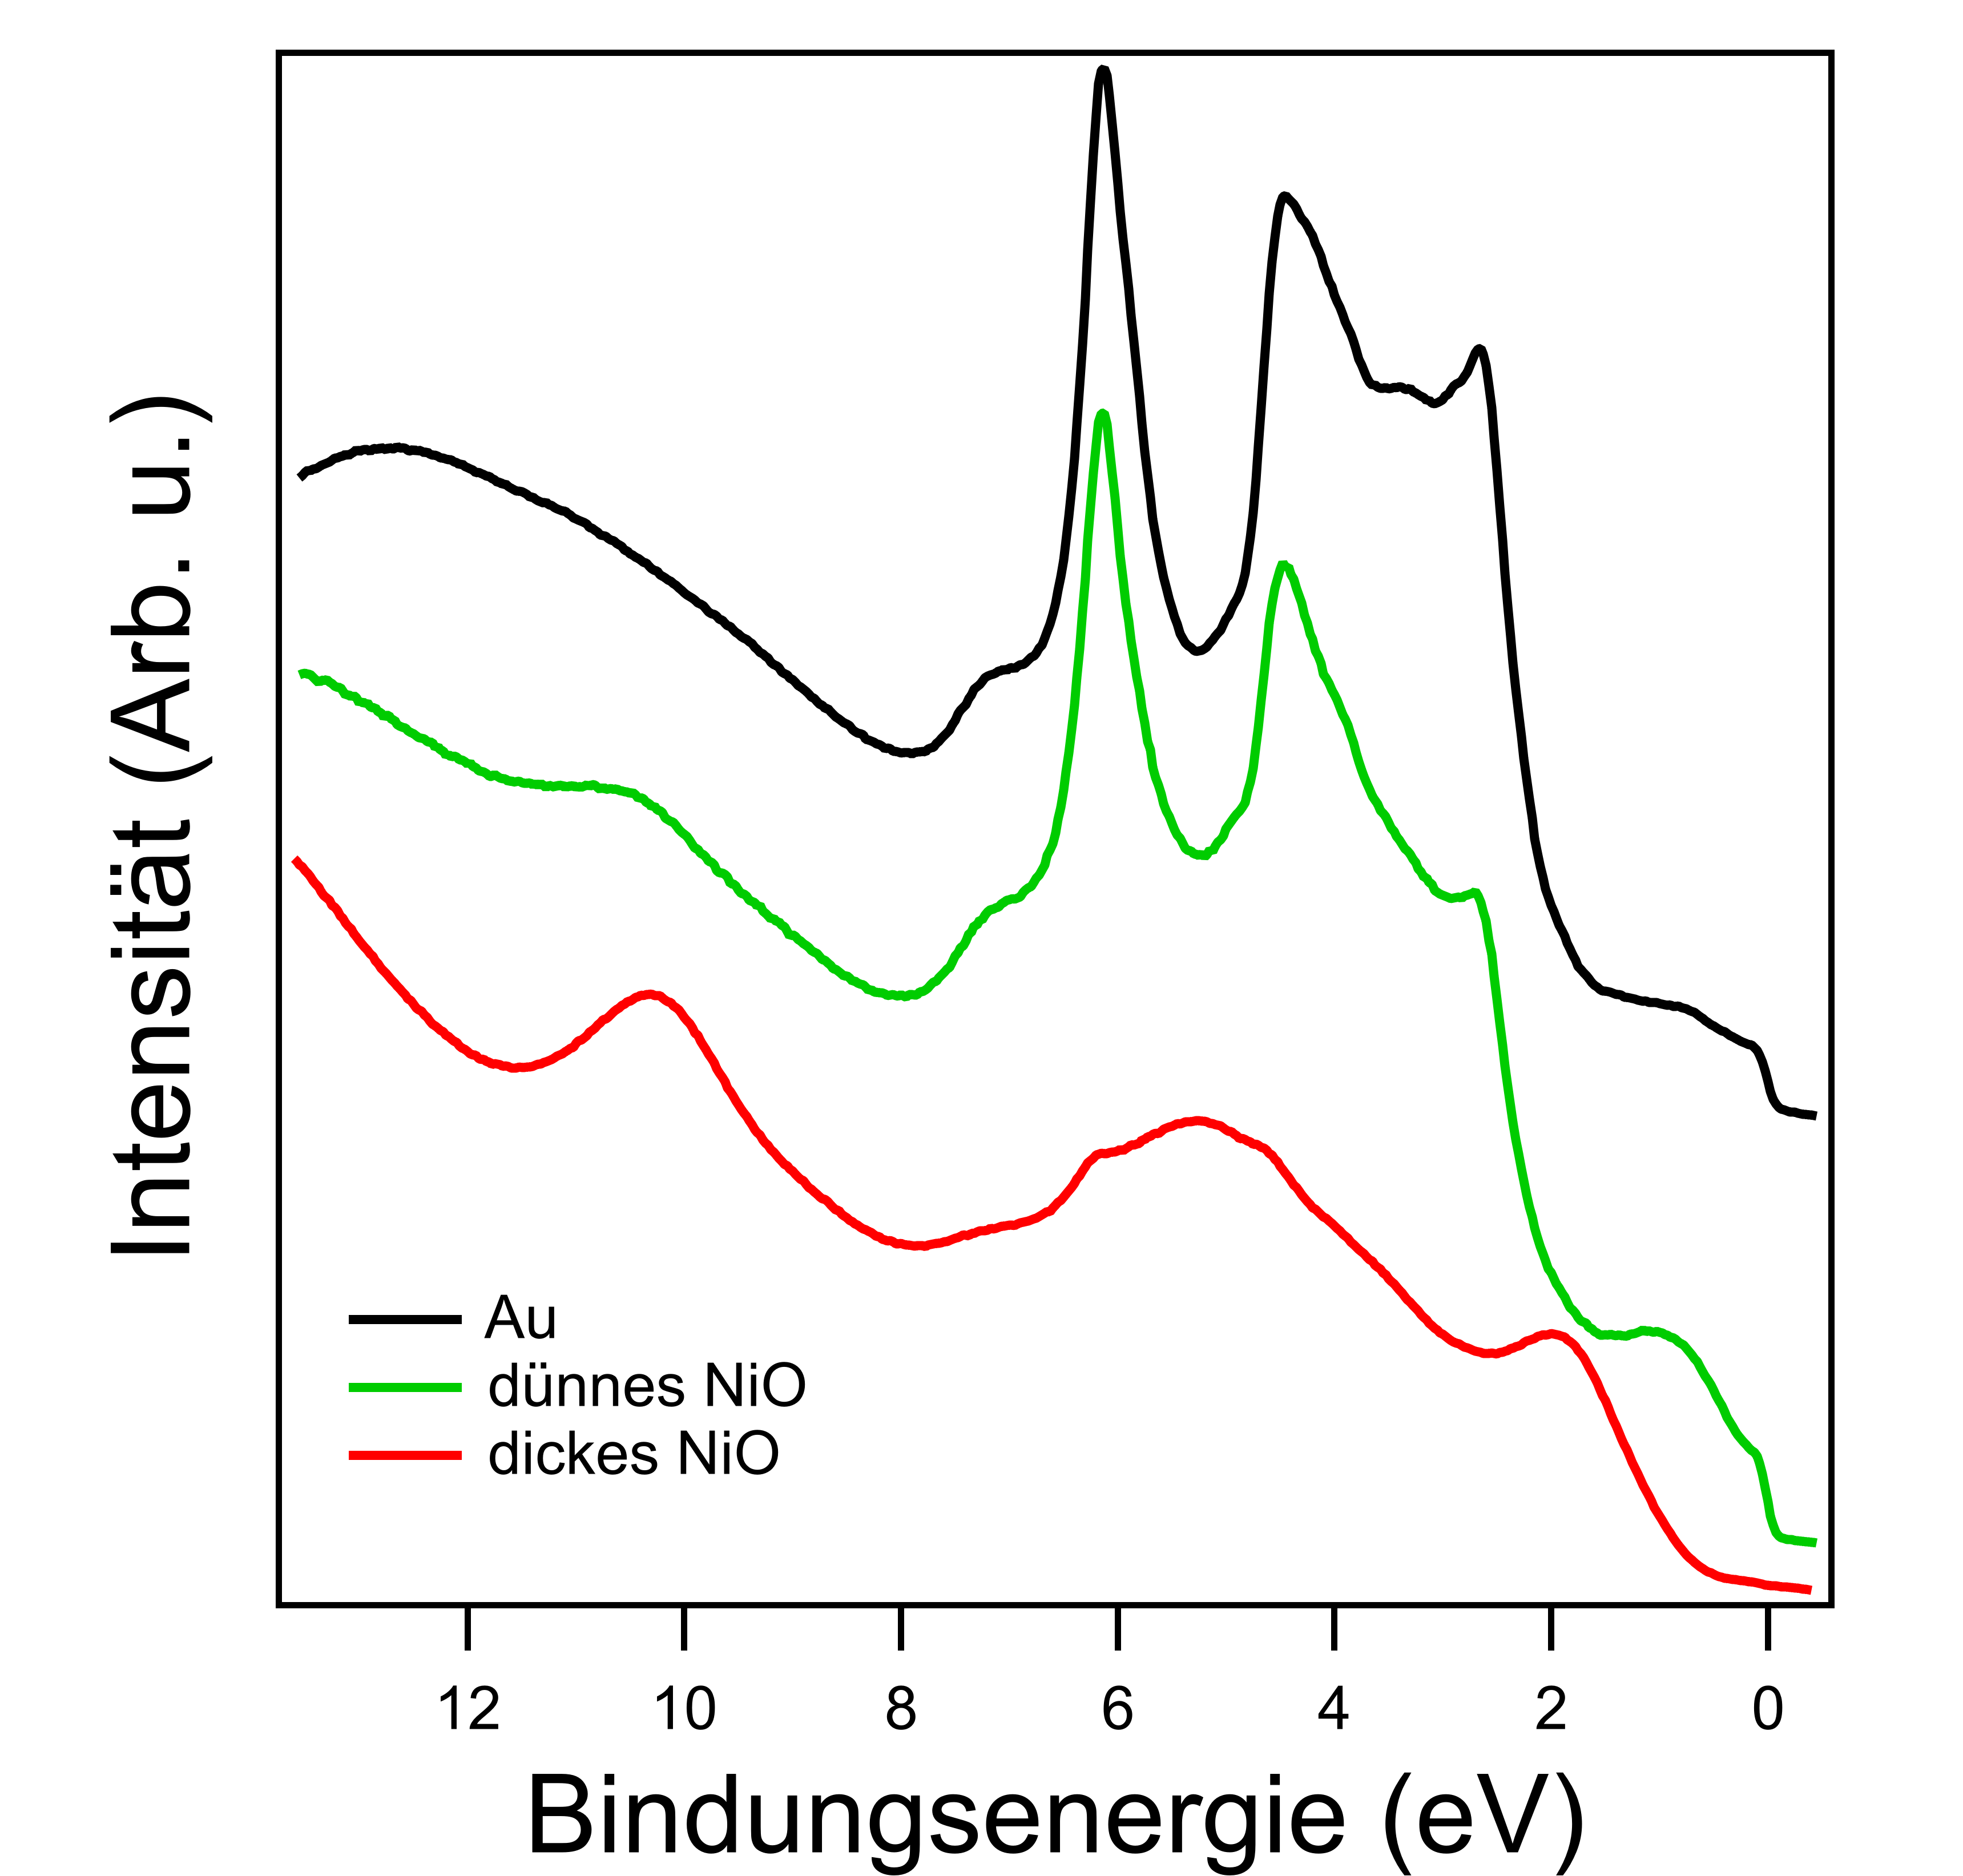
\includegraphics[height=5cm]{./content/pictures/NiO/NiO_Filmdicke.png}
                \subcaption{Die integrierten Spektren für zwei verschiedene Schichtdicken von \ce{NiO}. Als Referenz dient das integrierte Spektrum von Gold.}
                \label{fig:EDC_NiO}
            \end{subfigure}
            \begin{subfigure}[t]{0.48\textwidth}
                \centering
                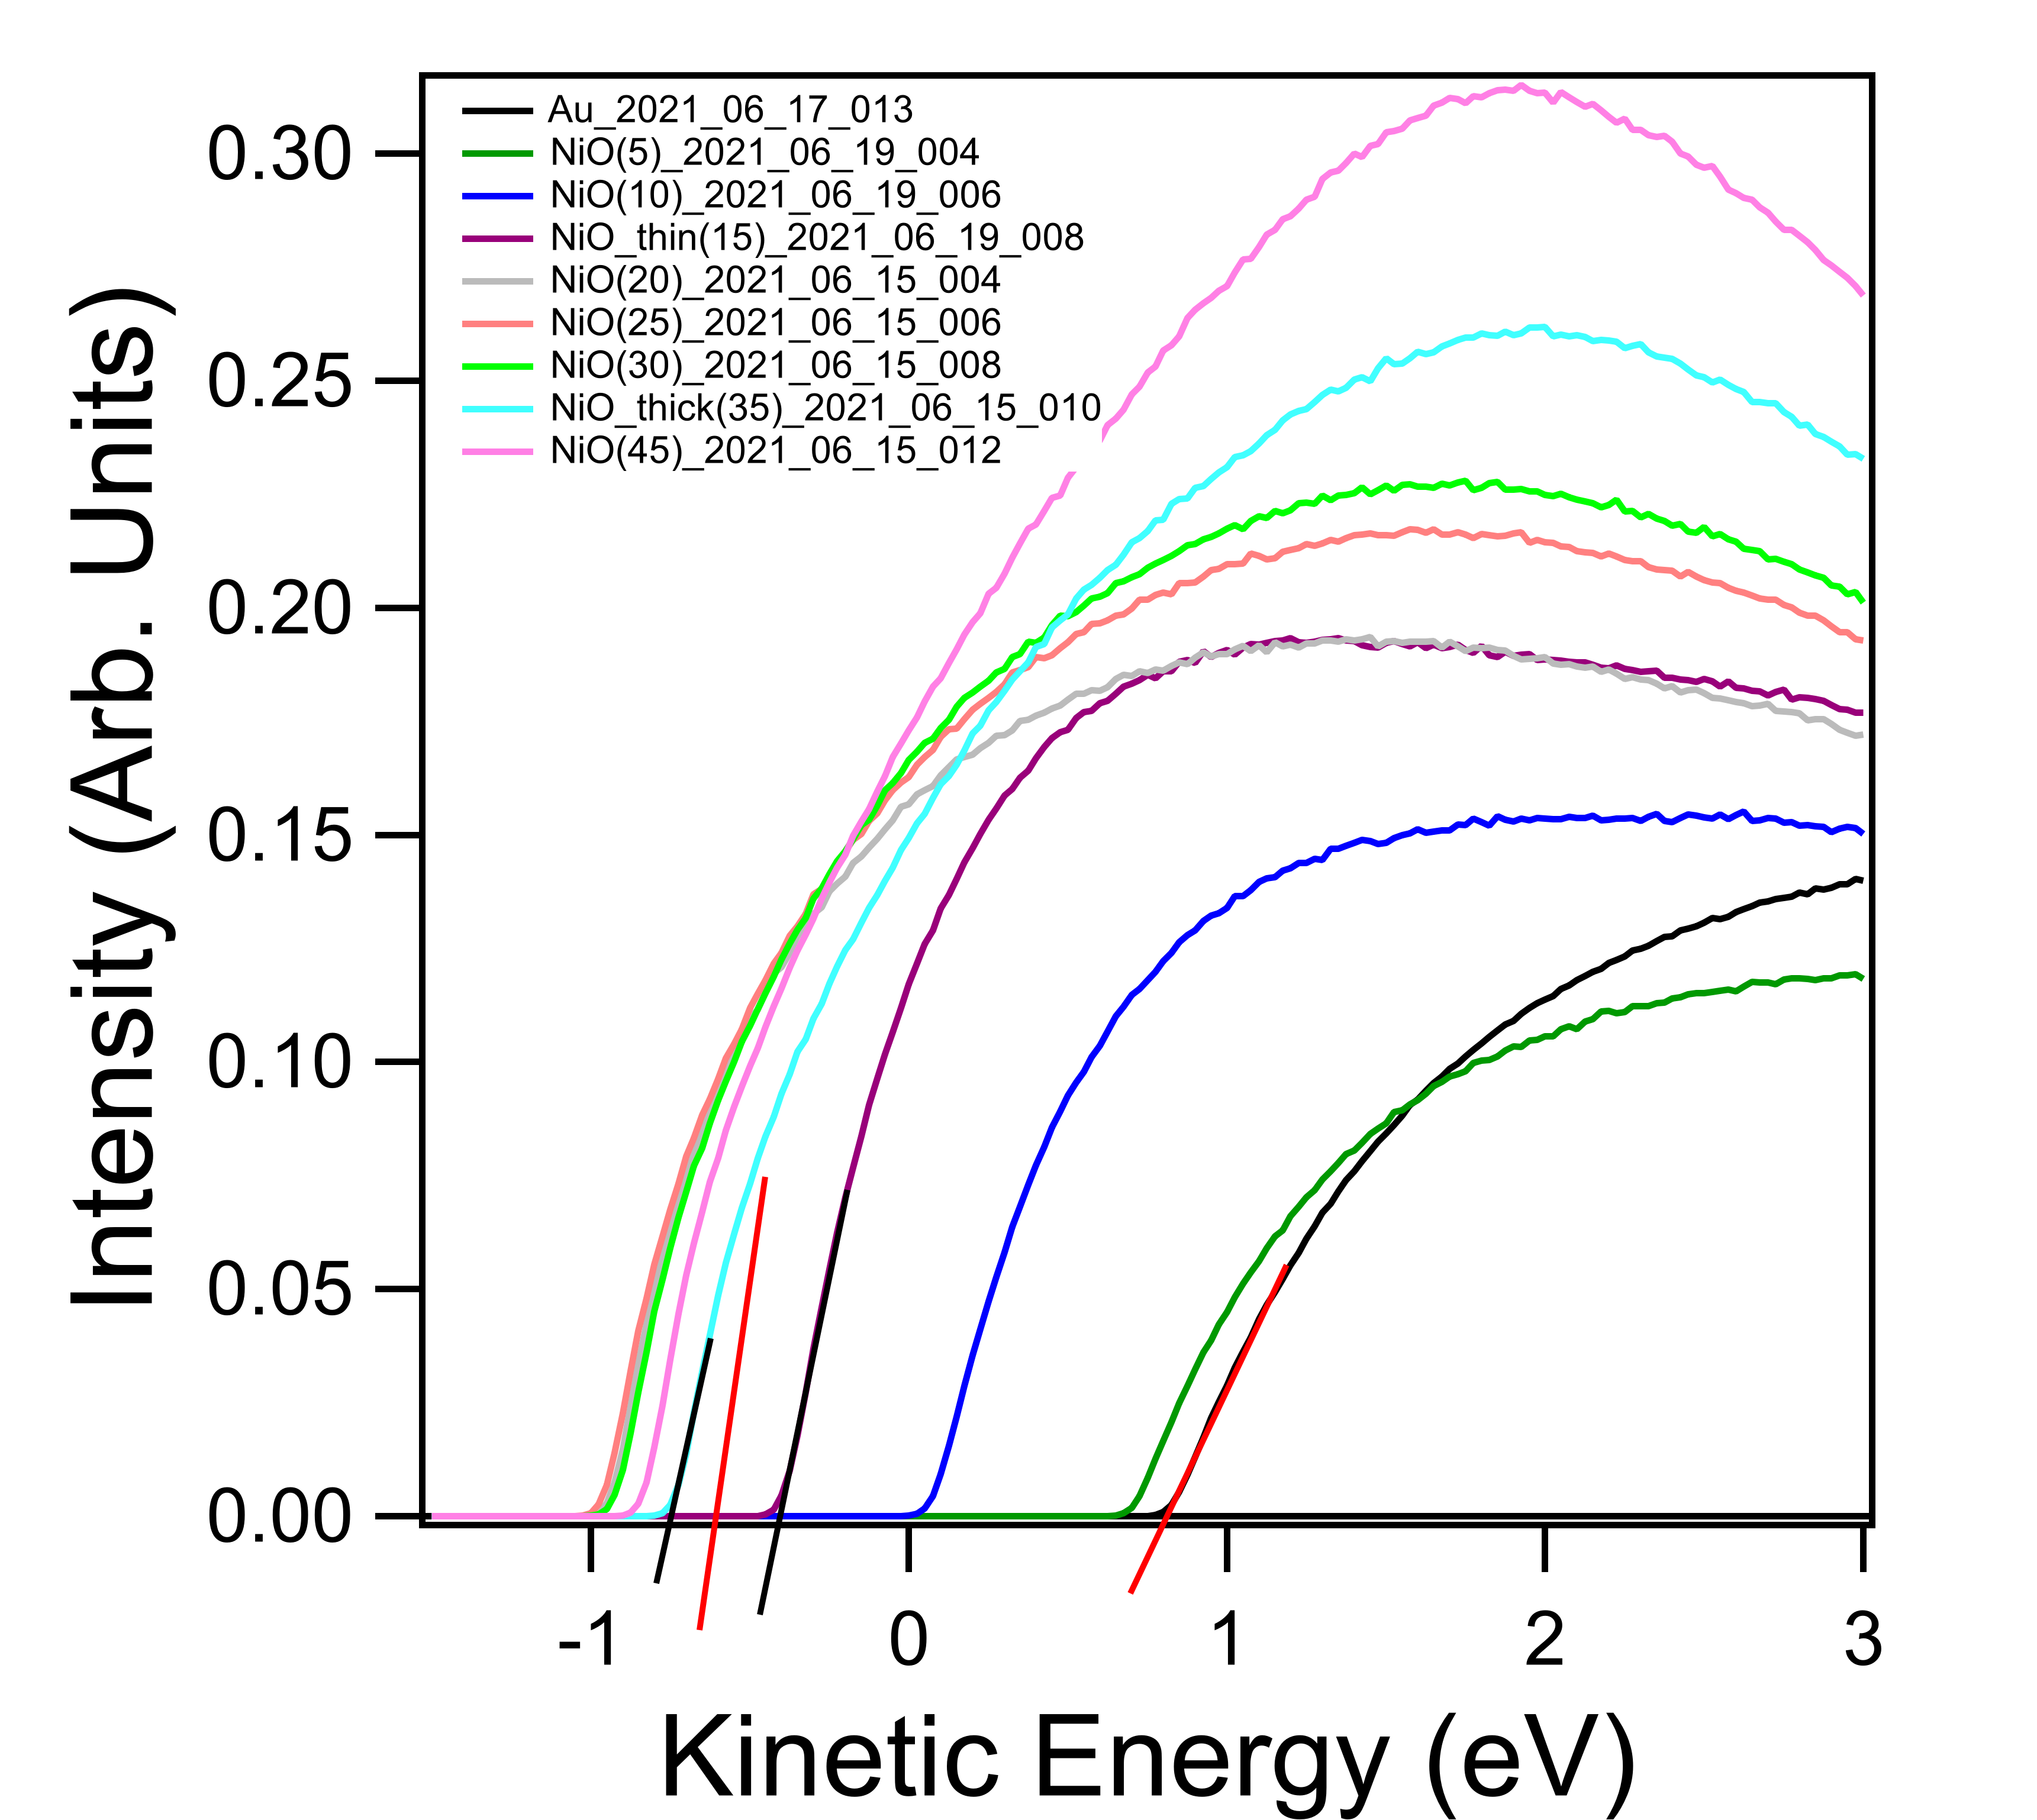
\includegraphics[height=5cm]{./content/pictures/NiO/NiO_WKF_thickness.png}
                \caption{Die integrierten Spektren im Bereich der Sekundärelektronen für verschiedene Schichtdicken von \ce{NiO}.}
                \label{fig:WKF_NiO}
            \end{subfigure}
            \caption{Integrierte Spektren für verschidene Schichtdicken und Bereiche des Nickeloxidfilms.}
        \end{figure}
        
        Durch Variation der Aufdampfzeiten lassen sich verschiedene Schichtdicken von Nickeloxidfilmen herstellen.
        Für zwei ausgewählte Zeiten sind die winkelintegrierten Spektren des Valenzbandbereiches in \autoref{fig:EDC_NiO} gemeinsam mit dem Spektrum des Substrates dargestellt.
        Zu erkennen ist, dass mit zunehmender Schichtdicke die charakteristischen Merkmale des Substrates abnehmen.
        Dafür steigt das Signal, was vom Nickeloxid herrührt an.
        Erkennbar ist somit auch die Oberflächenemfindlichkeit, der verwendeten Methode, da tiefer Lagen nur noch gering zum Signal beitragen.
        Aus der Verschiebung des Punktes an dem die Sekundärelektronen aufhören lässt sich erkennen, dass sich die Austrittsarbeit vom Gold zu dickeren Filmen Nickeloxid zu kleineren Werten verschiebt.
        Dies ist auch in \autoref{fig:WKF_NiO} für verschiedene Aufdampfzeiten dargestellt. 
        Kleine Verschiebungen können durch unterschiedliche Aufdampfbedingungen erklärt werden, denn es ist bekannt das durch Variation der Parameter gezielt die Eigenschaften manipuliert werden können.
        Vom dünnen Nickeloxidfilm zum dickeren Nickeloxidfilm wechselt sie von \SI{4.25}{\electronvolt} zu \SI{3.90}{\electronvolt}.
        Die Austrittsarbeit des dicken Nickeloxidfilms passt \textbf{oder passt nicht zu Quelle und Wert}.

        \begin{figure}
            \centering
            \begin{subfigure}[t]{0.48\textwidth}
                \centering
                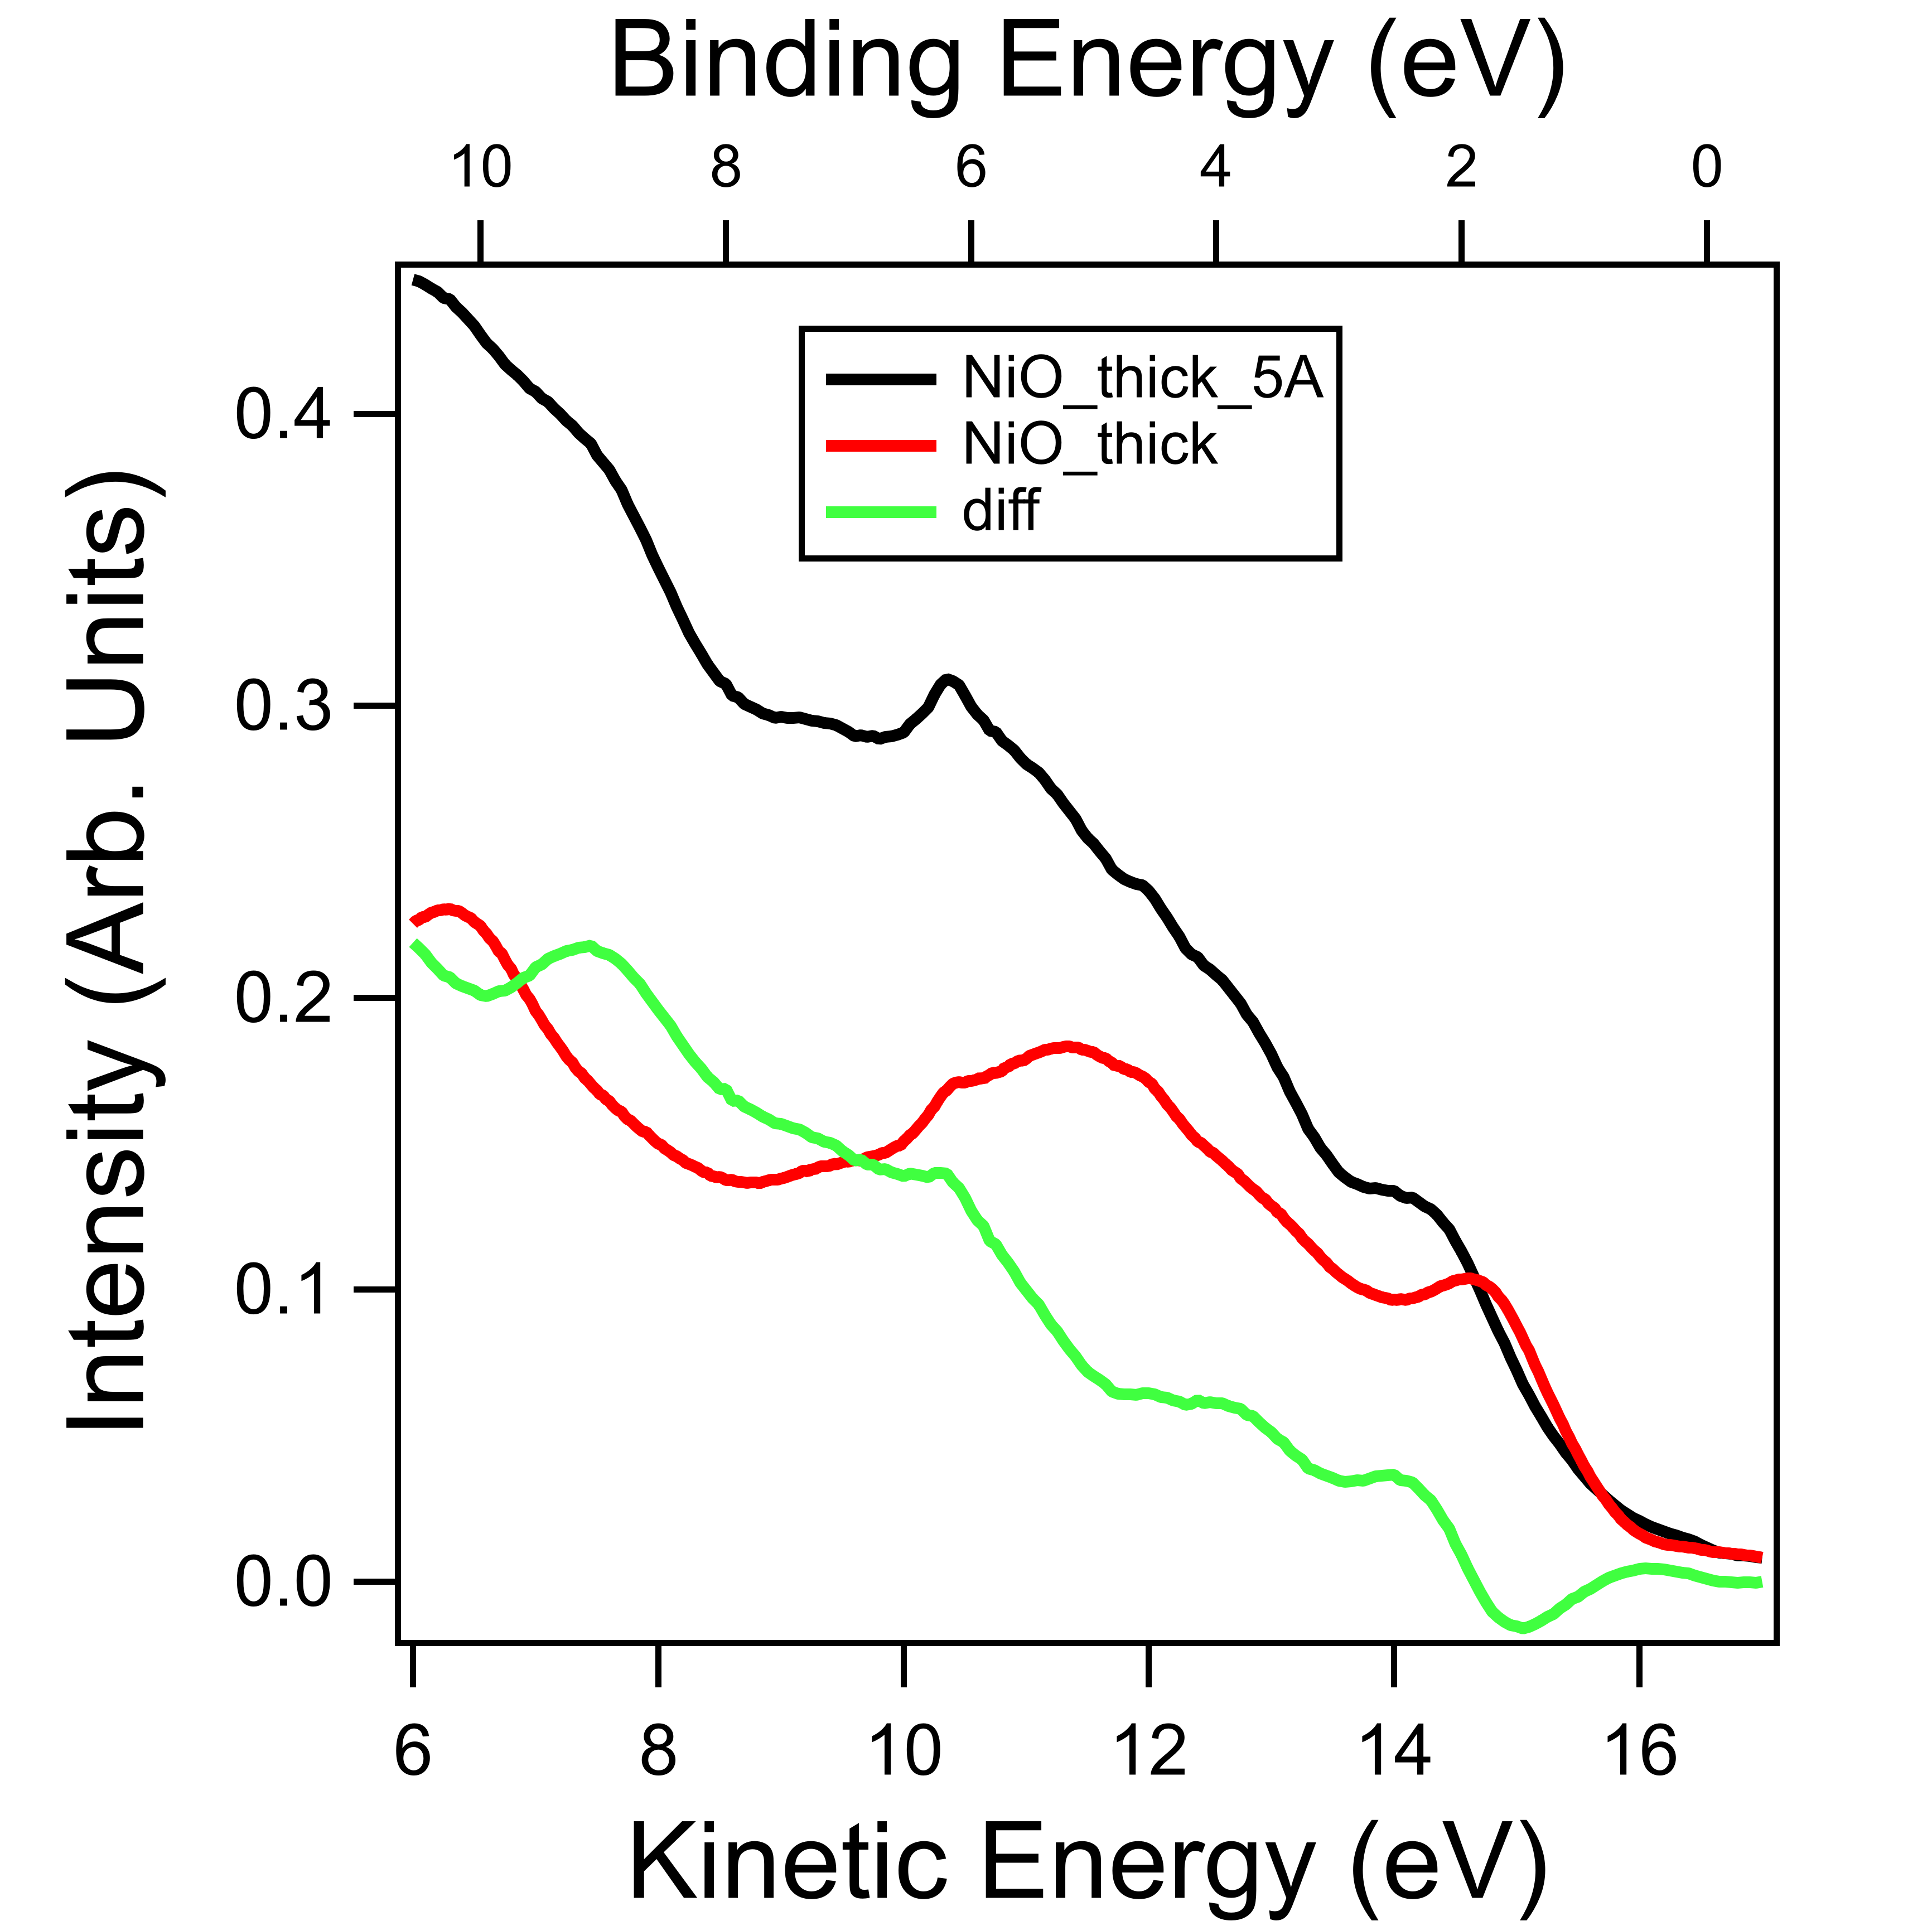
\includegraphics[height=5cm]{./content/pictures/NiO+5A/NiO_thick_5A.png}
                \subcaption{Die integrierten Spektren für einen dicken Nickeloxidfilm, mit zusaätzlich einer Monolage Pentacene und deren Differenz.}
                \label{fig:EDC_NiO+5A}
            \end{subfigure}
            \begin{subfigure}[t]{0.48\textwidth}
                \centering
                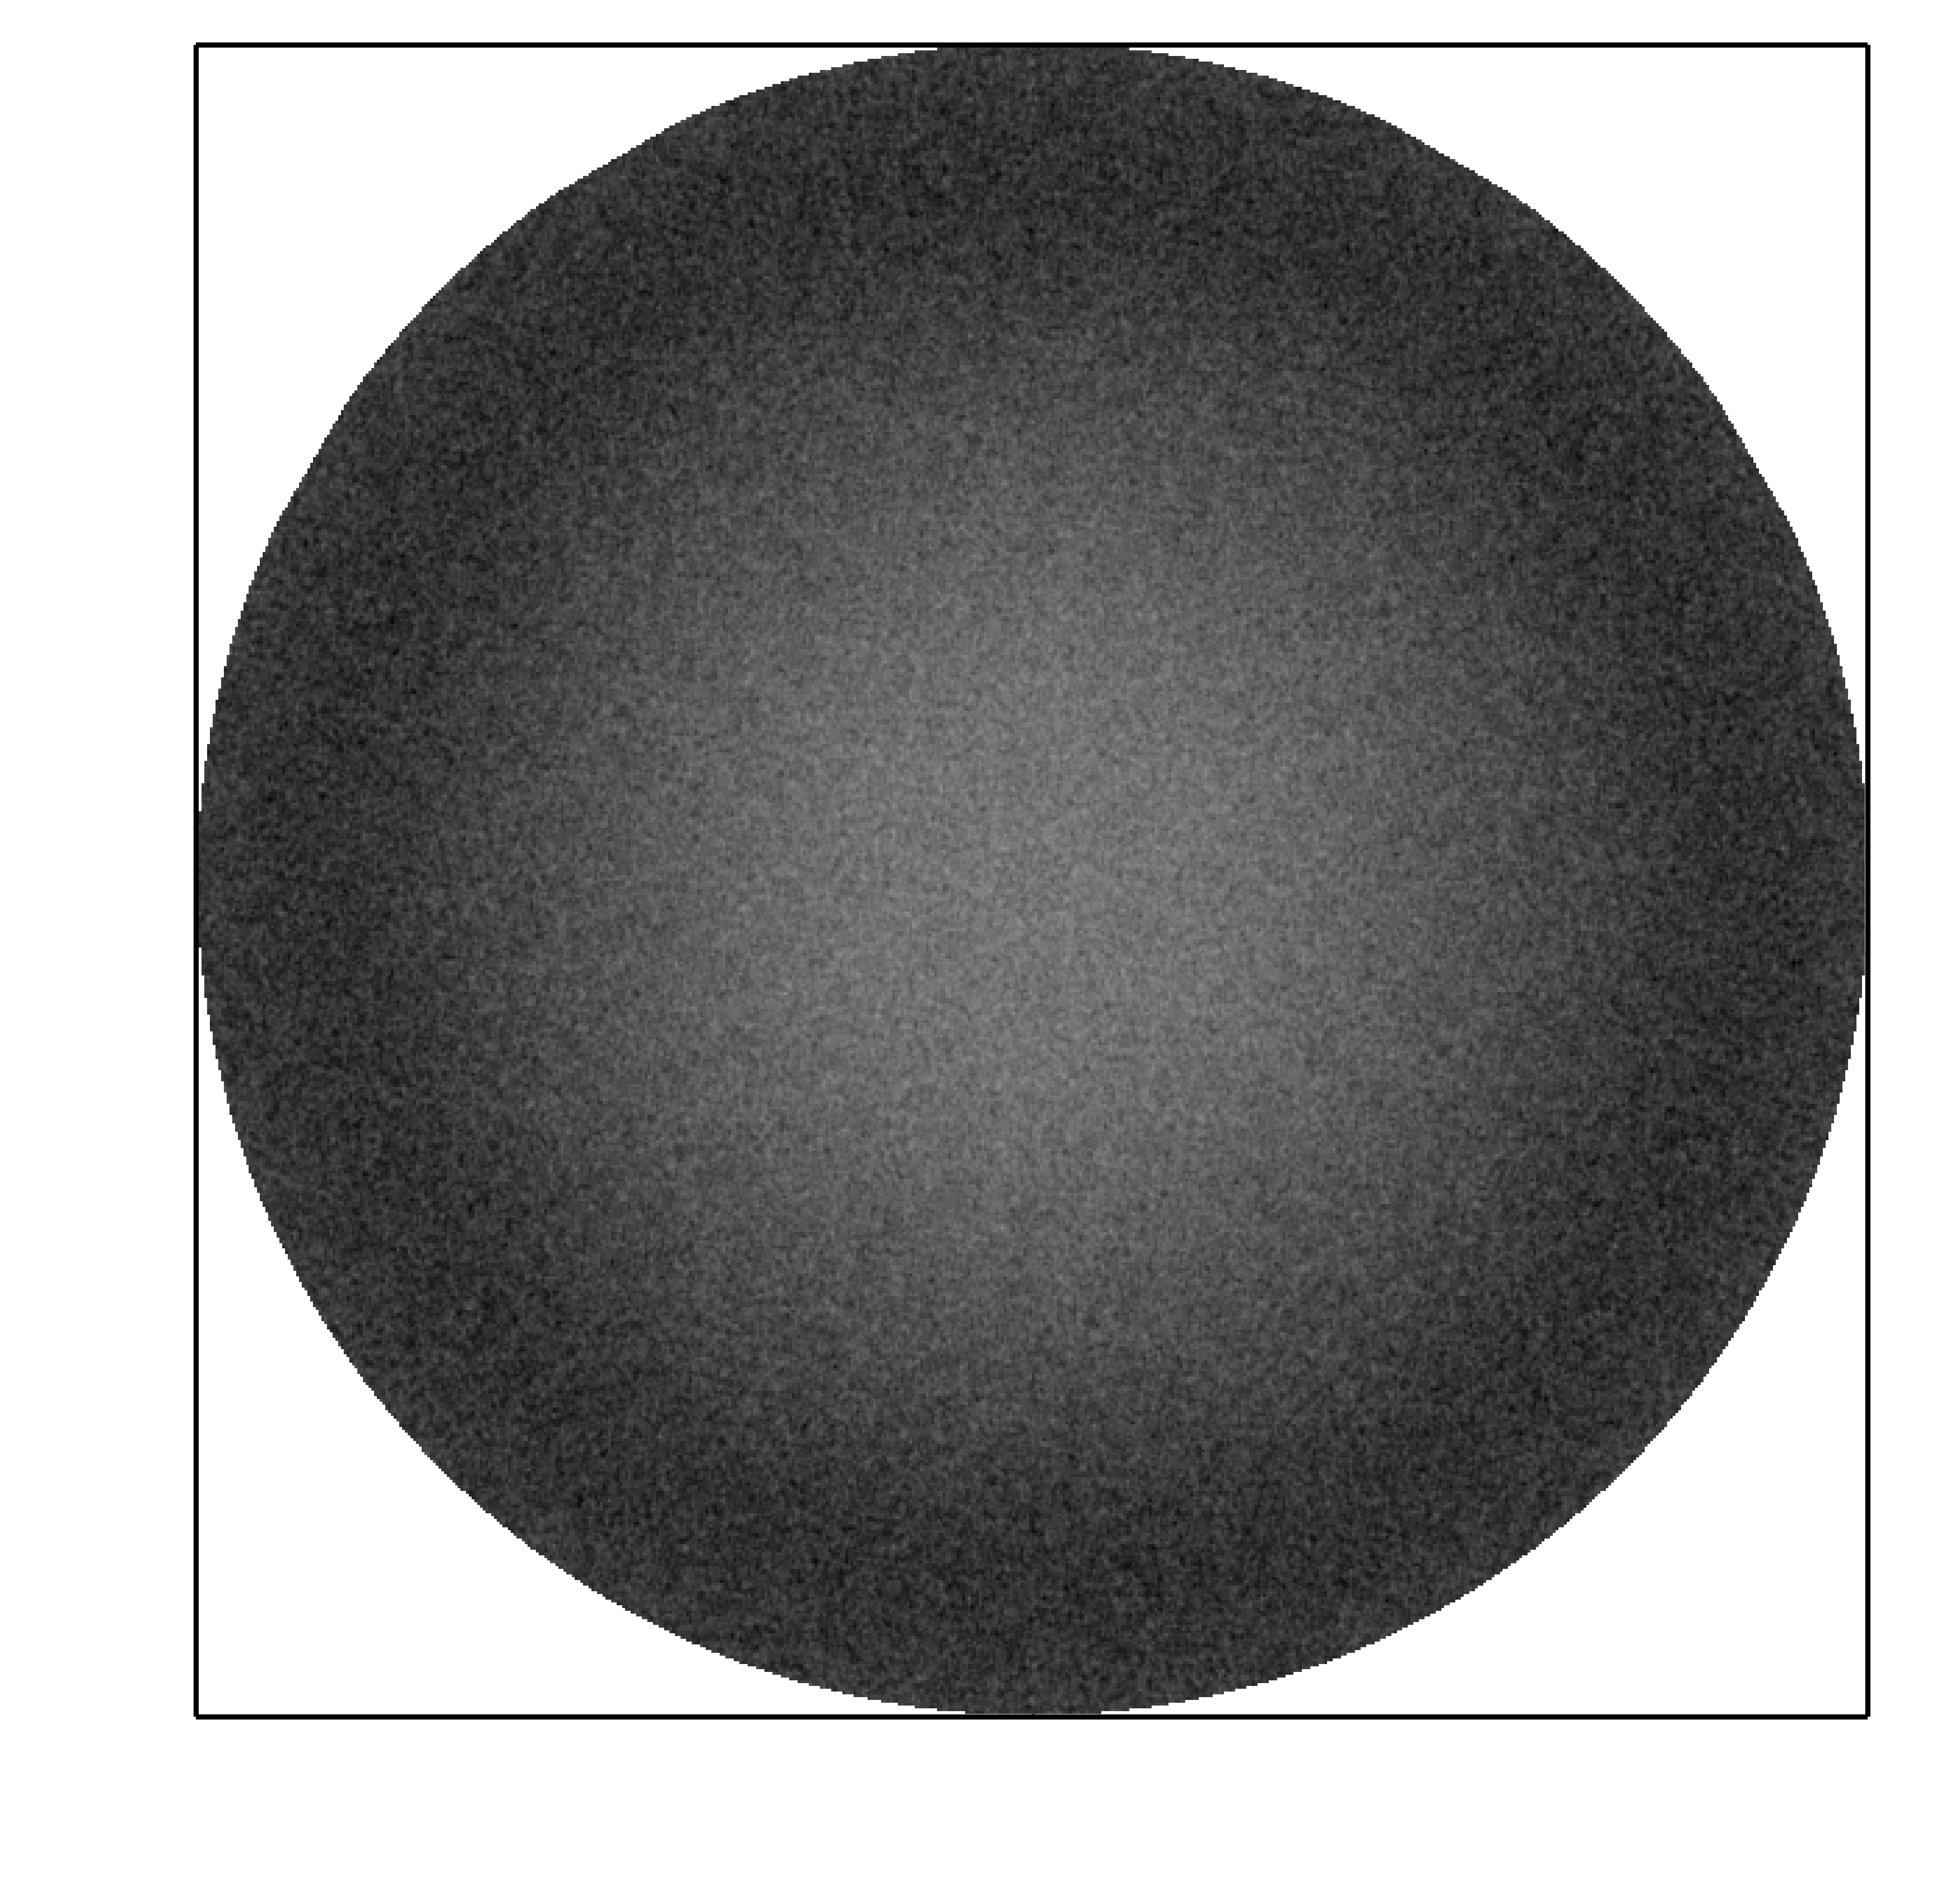
\includegraphics[height=5cm]{./content/pictures/NiO+5A/NiO_thick_5A_KE12_7.png}
                \subcaption{Map für Pentacene auf dicken Nickeloxidfilm bei einer kinetischen Energie von \SI{7.5}{\electronvolt}. Also Bindungsenergie von \SI{3.85}{\electronvolt}.}
                \label{fig:NiO+5A}
            \end{subfigure}
            \caption{Integriertes Spektrum des Valenzband Bereiches für reines Nickeloxid und mit einer Monolage Pentacene, sowie ein winkelaufgelöstes Bild.}
        \end{figure}
        Das Aufdampfen von einer Monolage Pentacene brachte kein LEED-Bild mehr zu stande.
        Nach dem Aufdampfen wurde versucht LEED-Bilder aufzunehmen, es waren allerdings nur leichte Substratspots sichtbar.
        So lässt sich schlussfolgern, dass sich die Moleküle auf der Oberfläche nicht anordnen.
        Dabei zeigt der direkte Vergleich der integrierten Spektren in \autoref{fig:EDC_NiO+5A} des reinen Nickeloxid und das mit Pentacene drauf deutliche zusätzliche Spitzen.
        Die Abwesenheit sehr ausgeprägter Merkmale in den impulsaufgelösten Bildern bestätigt die Annahme, dass sich die Moleküle auf der Oberfläche nicht regelmäßig anordnen.
        Ferner überlappen dann die einzelnen Merkmale im Impulsraum, sodass ein ausgewaschenes Bild entsteht.
        Auch wenn sich in den integrierten Spektren in \autoref{fig:EDC_NiO} klar zeigt, dass sich bei einigen Energien die Intensität erhöht ist in den entsprechenden Bildern keine klare Zuordnung möglich.
        Ein Beispiel ist in \autoref{fig:NiO+5A} zu sehen, dieses Bild wurde gewählt da ein deutliches Signal im integrierten Spektrum zu erkennen ist und die entsprechende Energie nicht zu weit weg von der Fermikante liegt.
        tendenziell sollten entsprechend winkelaufgelöste Bilder den theoretischen Berechnungen wie in \autoref{fig:MOT_Au+5A_theo} entsprechen, da Substrate gleiche Symmetrien aufweisen.
        \begin{itemize}
            \item WKF Shift für dicken
            \item NiO-Spektrum Peaks zuordnen
            \item linear ansteigender Untergrund bei Molekülen ? zu sehen in der Differenz
        \end{itemize}


    \section{Eisen}
        \begin{figure}
            \centering
            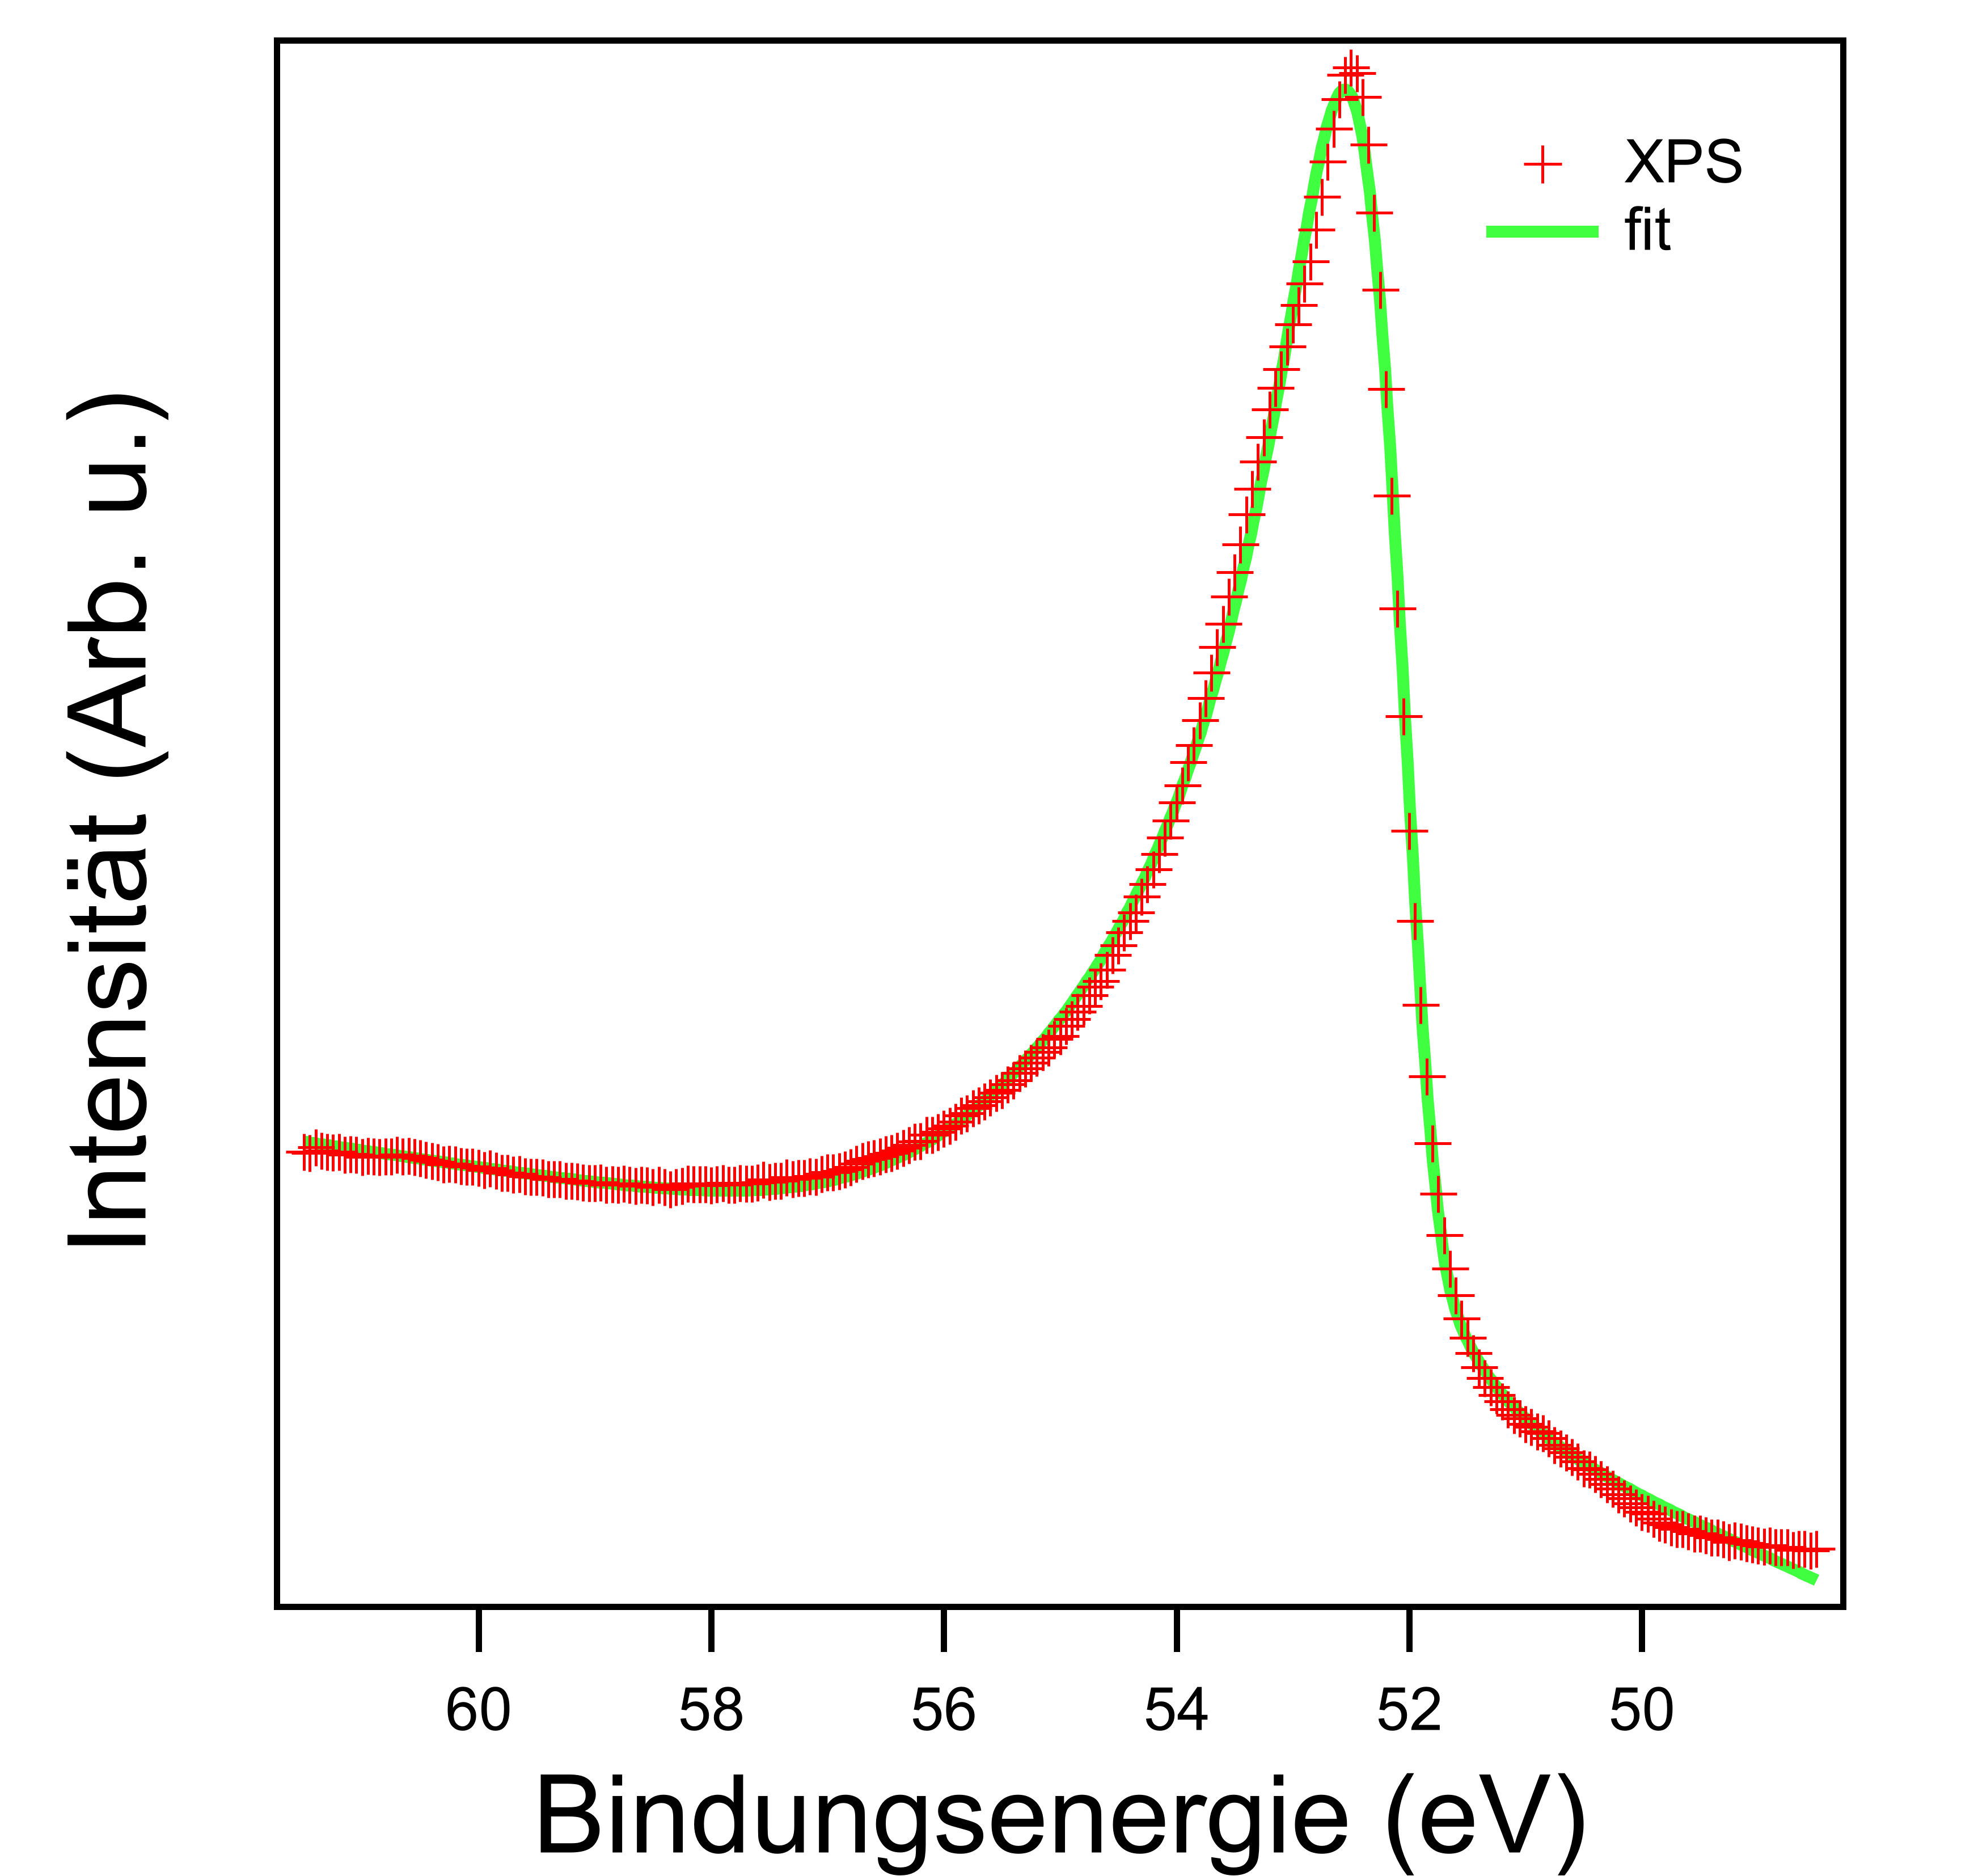
\includegraphics[width=0.5\textwidth]{./content/pictures/Fe/Fe3p_Fe.png}
            \caption{XPS Spektrum des $\ce{Fe}_{3\text{p}}$ Übergang des reinen Eisens. Hier passt der Fit mit einem Voigt (+Tougaard) sehr gut!}
            \label{fig:XPSFe3p_Fe}
        \end{figure}
        \begin{figure}
            \centering
            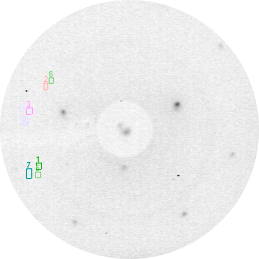
\includegraphics[height=5cm]{./content/pictures/pFe/2021_09_07_002_passivatedFe(100)_125eV.png}
            \caption{Passiviertes Eisen (100) bei einer Elektronenenergie von \SI{125}{\electronvolt}.}
            \label{fig:LEED_pFe}
        \end{figure}
        Bei der verwendeten Eisenprobe handelt es sich um einen dünnen Eisenfilm, der auf einem Magnesiumoxid Substrat gewachsen wurde.
        Die Probe wurde ebenfalls durch leichtes ioneninduziertes Zerstäuben und aufheizen auf \SI{600}{\celsius} gerreinigt.
        Die Reinheit der Probe lässt sich auch am Spektrum des $\ce{Fe}_{3\text{p}}$ Übergangs in \autoref{fig:XPSFe3p_Fe} erkennen.
        Das Signal bei \SI{52.83}{\electronvolt} lässt sich nach Abzug eines Pseudo-Tougaard Untergrund sehr gut mit einer Pseudo-Voigt Funktion approximieren.
        Entsprechend gab sich die Halbwertsbreite zu \SI{2.11}{\electronvolt}.
        Um Verunreinigungen des sehr reaktiven sauberen Eisens zu vermeiden, wird die Probe anschließend direkt passiviert.
        Dies geschieht in einer Sauerstoffatmosphäre von \SI{1.3e-7}{\milli\bar} für fünf Minuten, während die Probe bei \SI{550}{\celsius} gehalten wird.
        Die Probe wird dann nocheinmal kurz auf \SI{600}{\celsius} aufgeheizt.
        Nun wird auch dessen Oberflächenbeschaffenheit kontrolliert und entsprechendes LEED-Bild ist in \autoref{fig:LEED_pFe} zu sehen.
        Sie Spots sind scharf und zeigen auch die Geometrie der $\ce{Fe}-\text{p}(1 \times 1)\ce{O}$ Struktur.
        Die gesamten Spots sind dabei nicht zentrosymmetrisch, da die Probe verkippt ist, wodurch auch der (0,0)-Reflex zu sehen ist.

        \begin{figure}
            \centering
            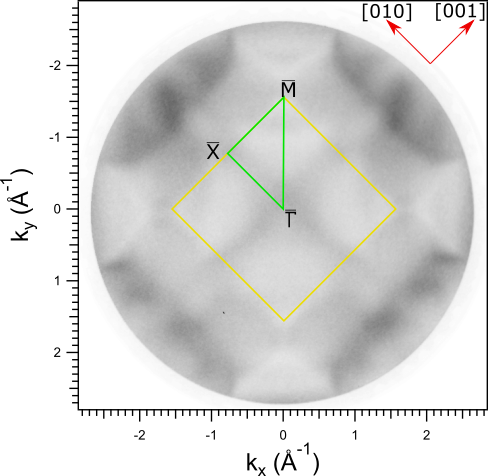
\includegraphics[width=0.5\textwidth]{./content/pictures/Fe/BZ_Fe.png}
            \caption{Die Brillouinzone des reinen Eisens bei einer Bindungsenergie von \SI{0.3}{\electronvolt}.
            Eigezeichnet sind auch die Vektoren, sowie einige Hochsymmetrierichtungen.
            Die Kantenlänge der BZ ist $\frac{2\pi}{a} = \SI[per-mode=reciprocal]{2.20}{\per\angstrom}$.
            Im Zentrum liegt der $\overline{\Gamma}$-Punkt, der Abstand zum $\overline{X}$-Punkt ist $\frac{2\pi}{2 \cdot a} = \SI[per-mode=reciprocal]{1.10}{\per\angstrom}$ und zum $\overline{M}$-Punkt $\frac{2\pi}{2 \cdot a} \sqrt{2} = \SI[per-mode=reciprocal]{1.55}{\per\angstrom}$.}
            \label{fig:BZ_Fe}
        \end{figure}
        Wie schon für das Gold lässt sich auch die Oberflächenbrillouinzone des Eisens darstellen. 
        Dies ist in \autoref{fig:BZ_Fe} geschehen.
        Aus ihr lässt sich dann anschließend wieder die Bandstruktur extrahieren.
        

    \section{Magnetit}
        \begin{figure}
            \centering
            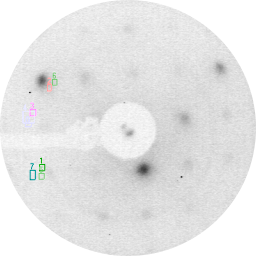
\includegraphics[height=5cm]{./content/pictures/Fe3O4/2021_09_07_012_FeO(100)_44eV.png}
            \caption{\ce{Fe3O4} (100) bei einer Elektronenenergie von \SI{44}{\electronvolt}.}
            \label{fig:LEED_Fe3O4}
        \end{figure}
        Auf dem der passivierten Eisenoberfläche wird Eisen mit einer Rate von \SI{0.6}{\ML\per\minute} und einem Sauerstoffdruck von \SI{2e-7}{\milli\bar} aufgedampft.
        Dabei wird die Probe auf eine Temperatur von \SI{230}{\celsius} gehalten.
        Zum abschluss wird die Temperatur auf \SI{600}{\degree} für fünf Minuten erhöht.
        So ergibt sich in \autoref{fig:LEED_Fe3O4} das Beugungsbild der Oberfläche.

        \begin{figure}
            \centering
            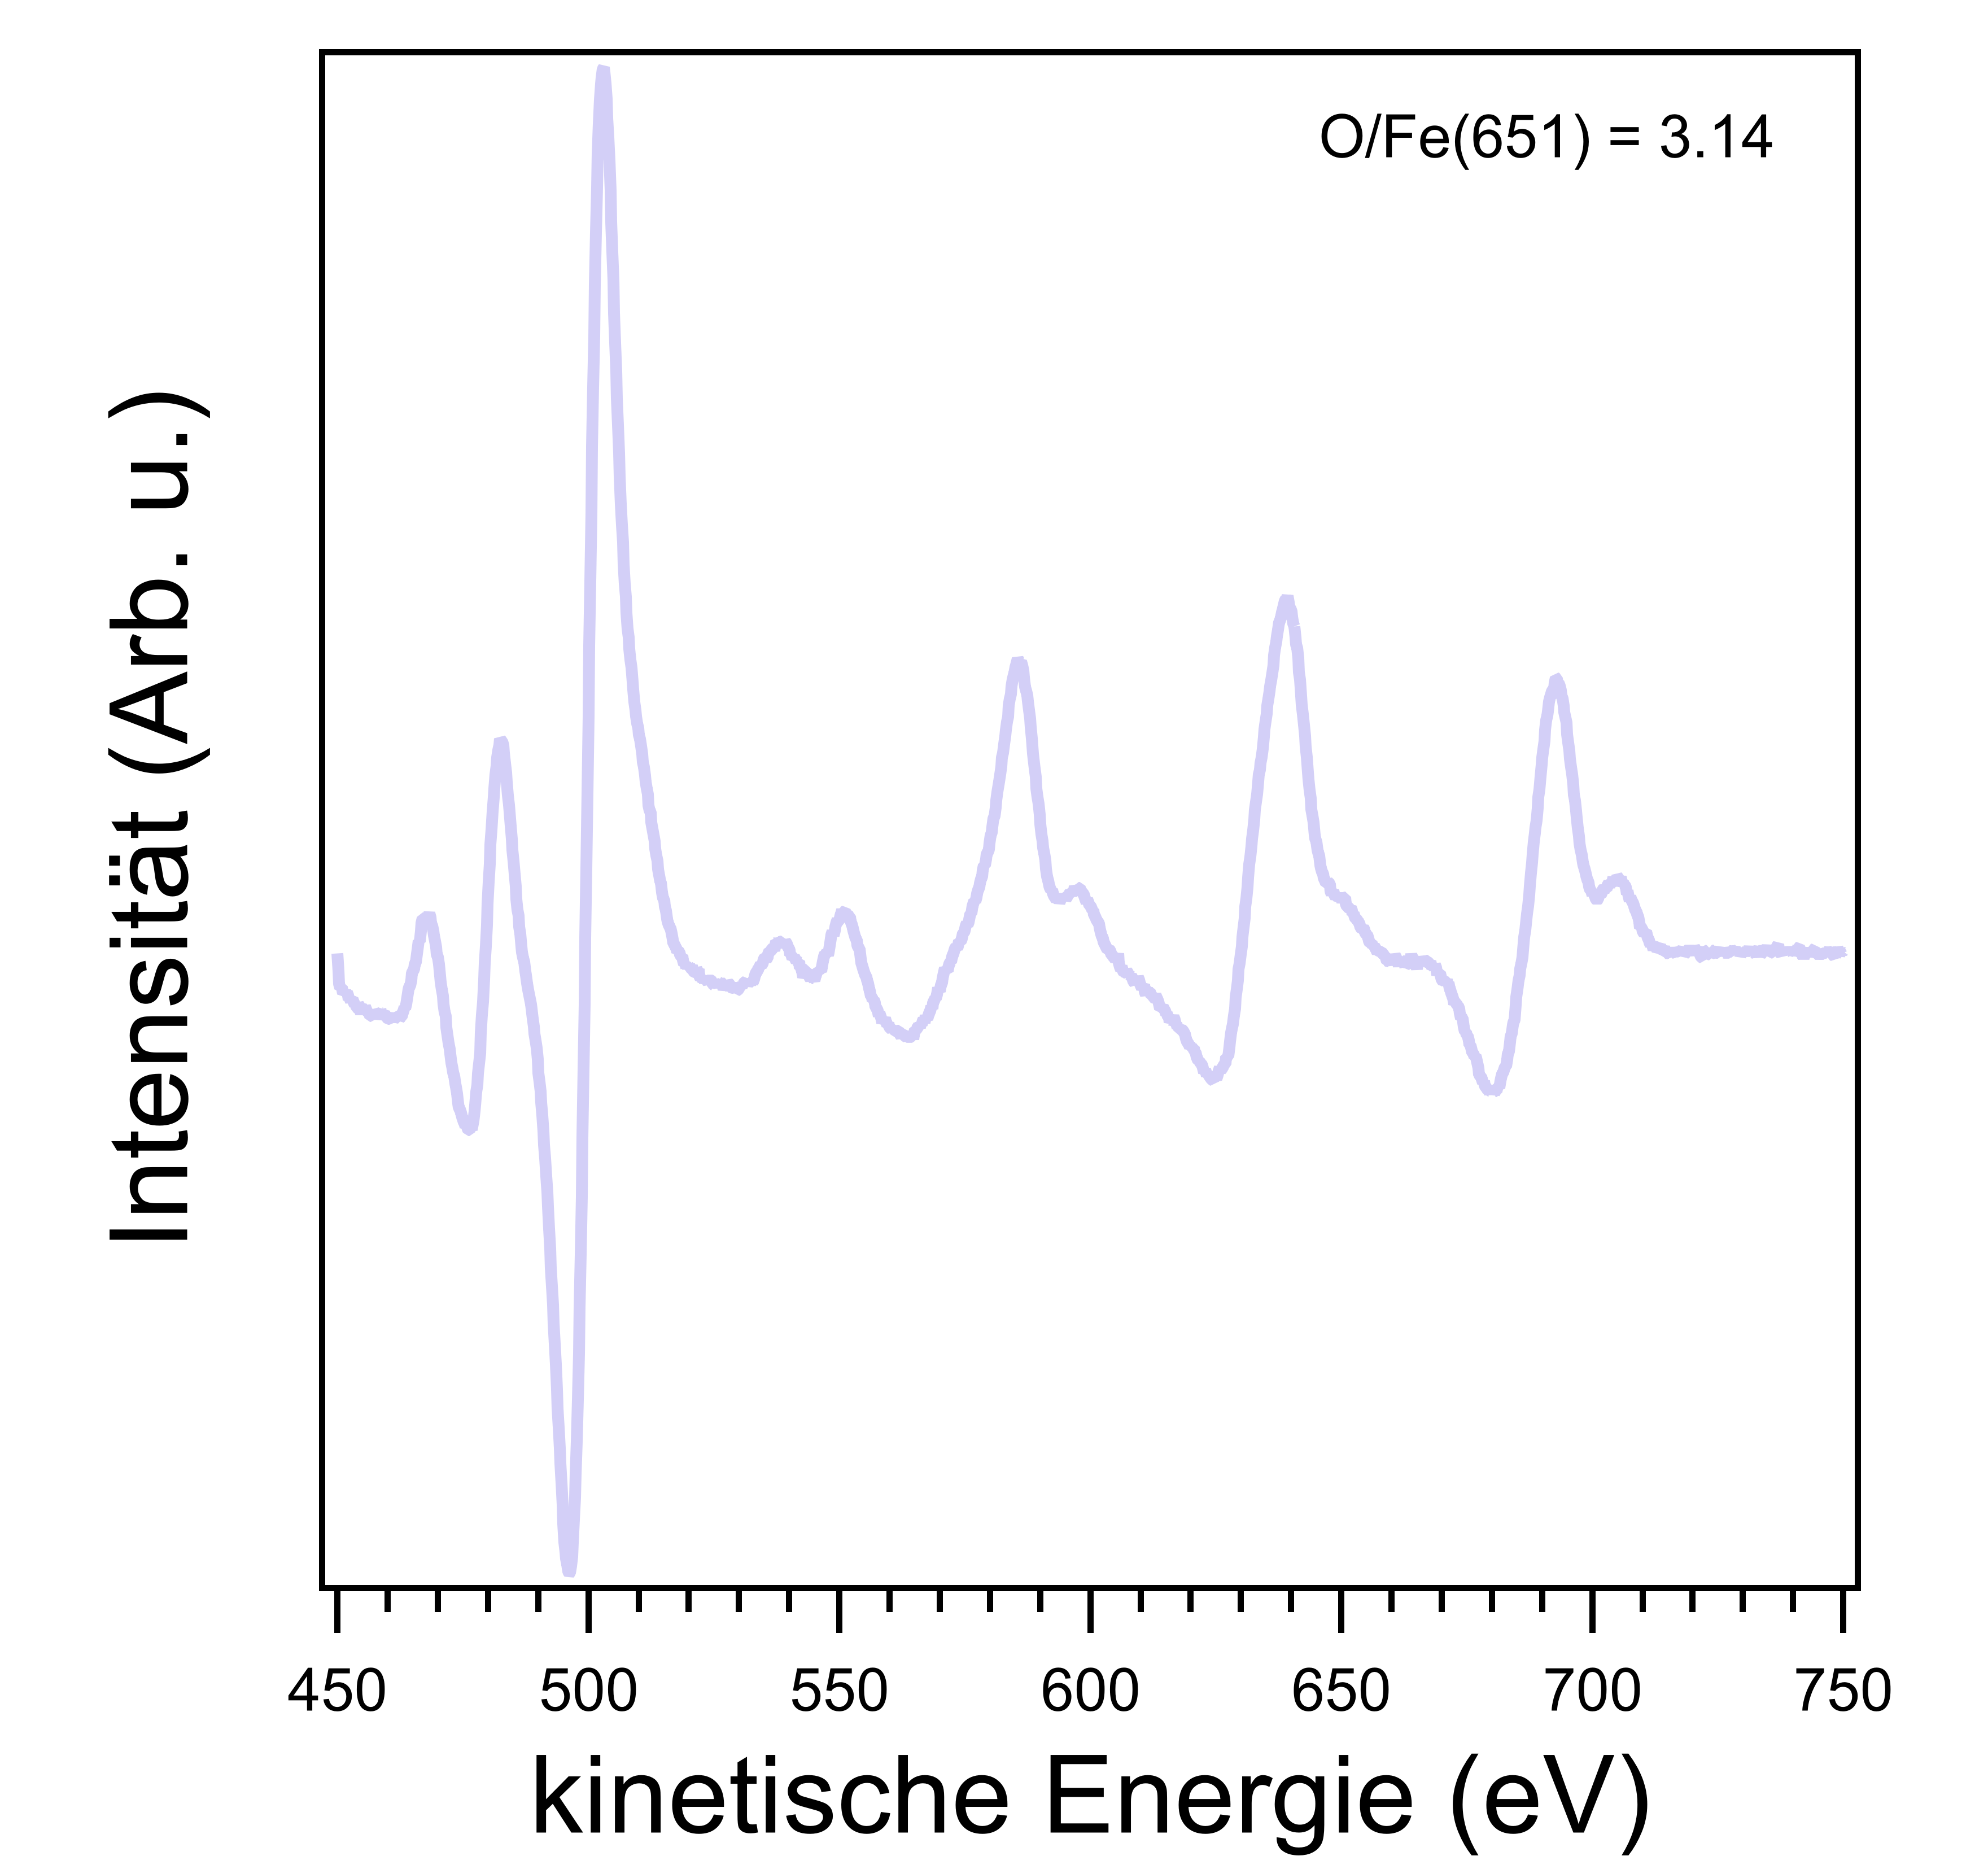
\includegraphics[height=5cm]{./content/pictures/Fe3O4/AES_Fe3O4.png}
            \caption{Das Augerspektrum der Magnetitprobe.}
            \label{fig:Auger_Fe3O4}
        \end{figure}
        Die Konzentrationen an Sauerstoff und Eisen werden mittels Augerelektronenspektroskopie analysiert.
        So ergibt sich das Augerspektrum in \autoref{fig:Auger_Fe3O4}.
        Das Peakverhältnis zwischen dem Sauerstoffsignal bei \SI{503}{\electronvolt} und dem Signal für Eisen bei \SI{651}{\electronvolt} ergibt einen Wert von \num{3.14}~\cite{FeO_1, Auger}.
        Aus der Literatur ist bekannt das für Magnetit ein Wert von \num{3.86} erwartet wird~\cite{FeO_1}.
        Der ermittelte Wert weicht dabei nach unten ab, was durch das zusätzliche Aufheizen auf \SI{600}{\degree} erklärt werden kann.
        Dabei kommt es zur Umstrukturierung der Oberfläche und in Folge dessen auch zur Desorption von Sauerstoff.

        \begin{figure}
            \centering
            \begin{subfigure}[t]{0.48\textwidth}
                \centering
                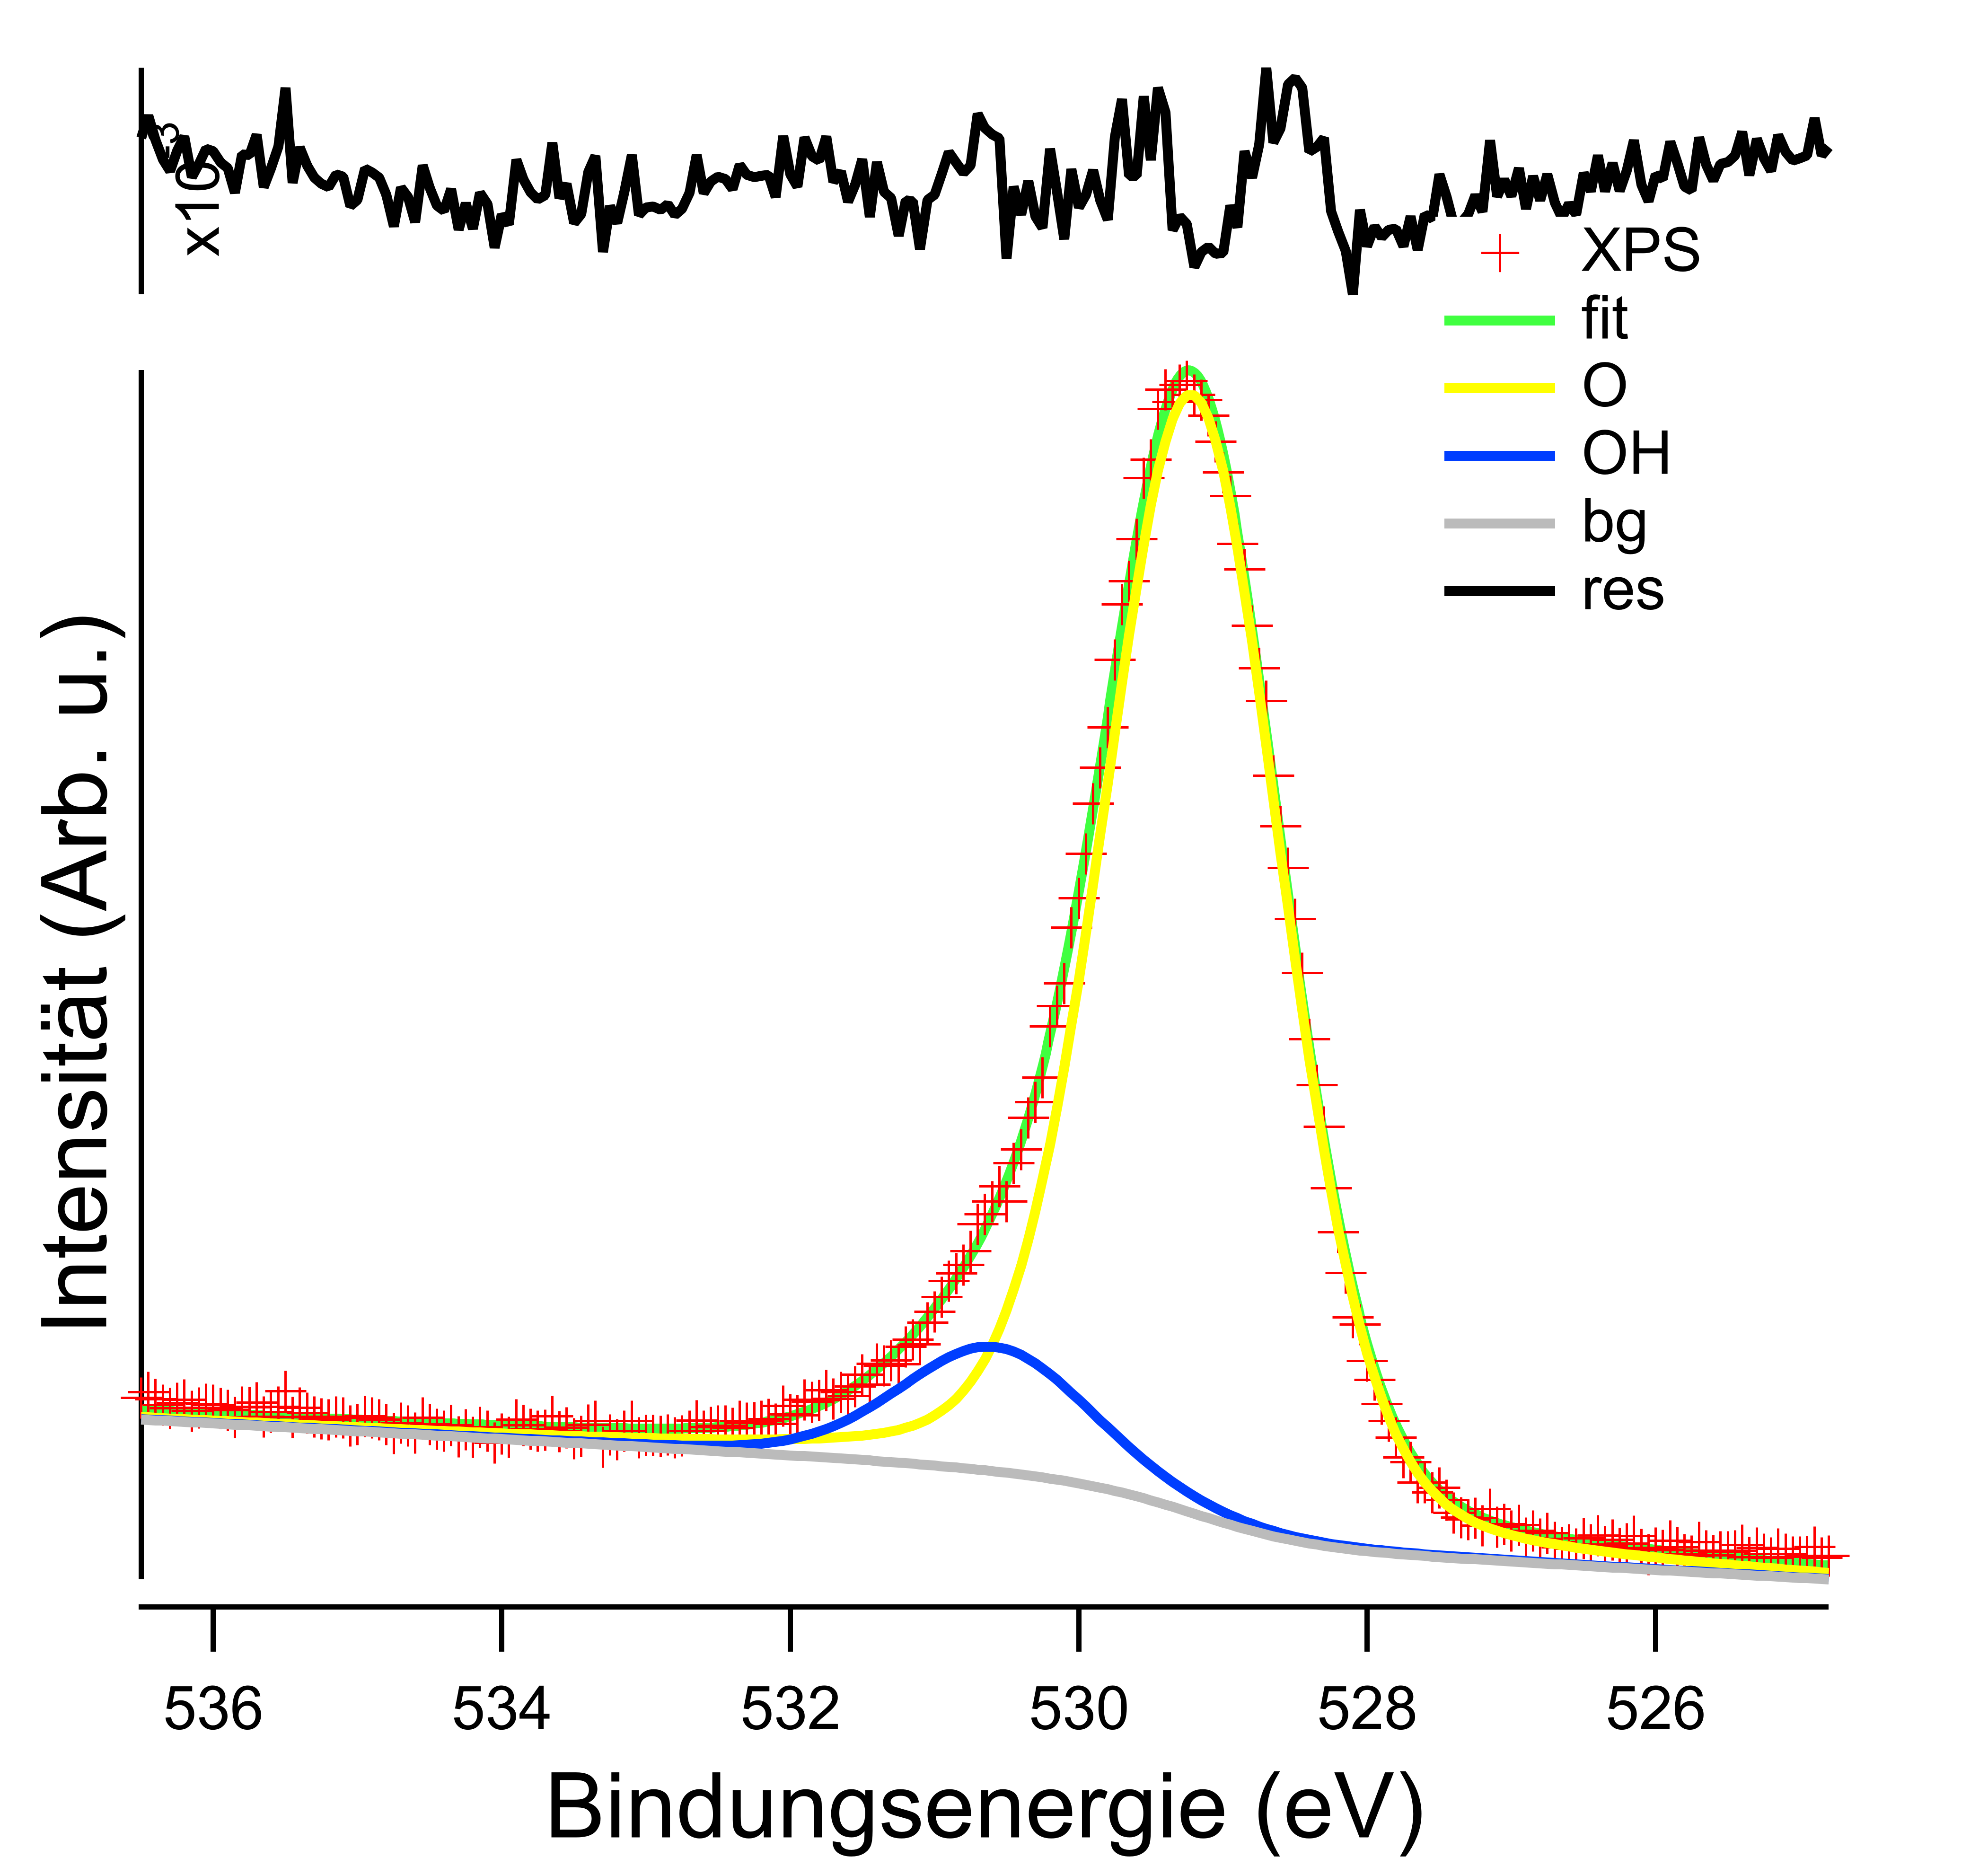
\includegraphics[height=5cm]{./content/pictures/Fe3O4/O1s_Fe3O4.png}
                \subcaption{Spektrum des $\ce{O}_{1\text{s}}$ Übergang. Fit mit zwei Peaks (kleiner Shirley) sehr gut (einer O, der andere OH - Kontamination evtl vom Aufdampfen?).}
                \label{fig:XPSO1s_Fe3O4}
            \end{subfigure}
            \begin{subfigure}[t]{0.48\textwidth}
                \centering
                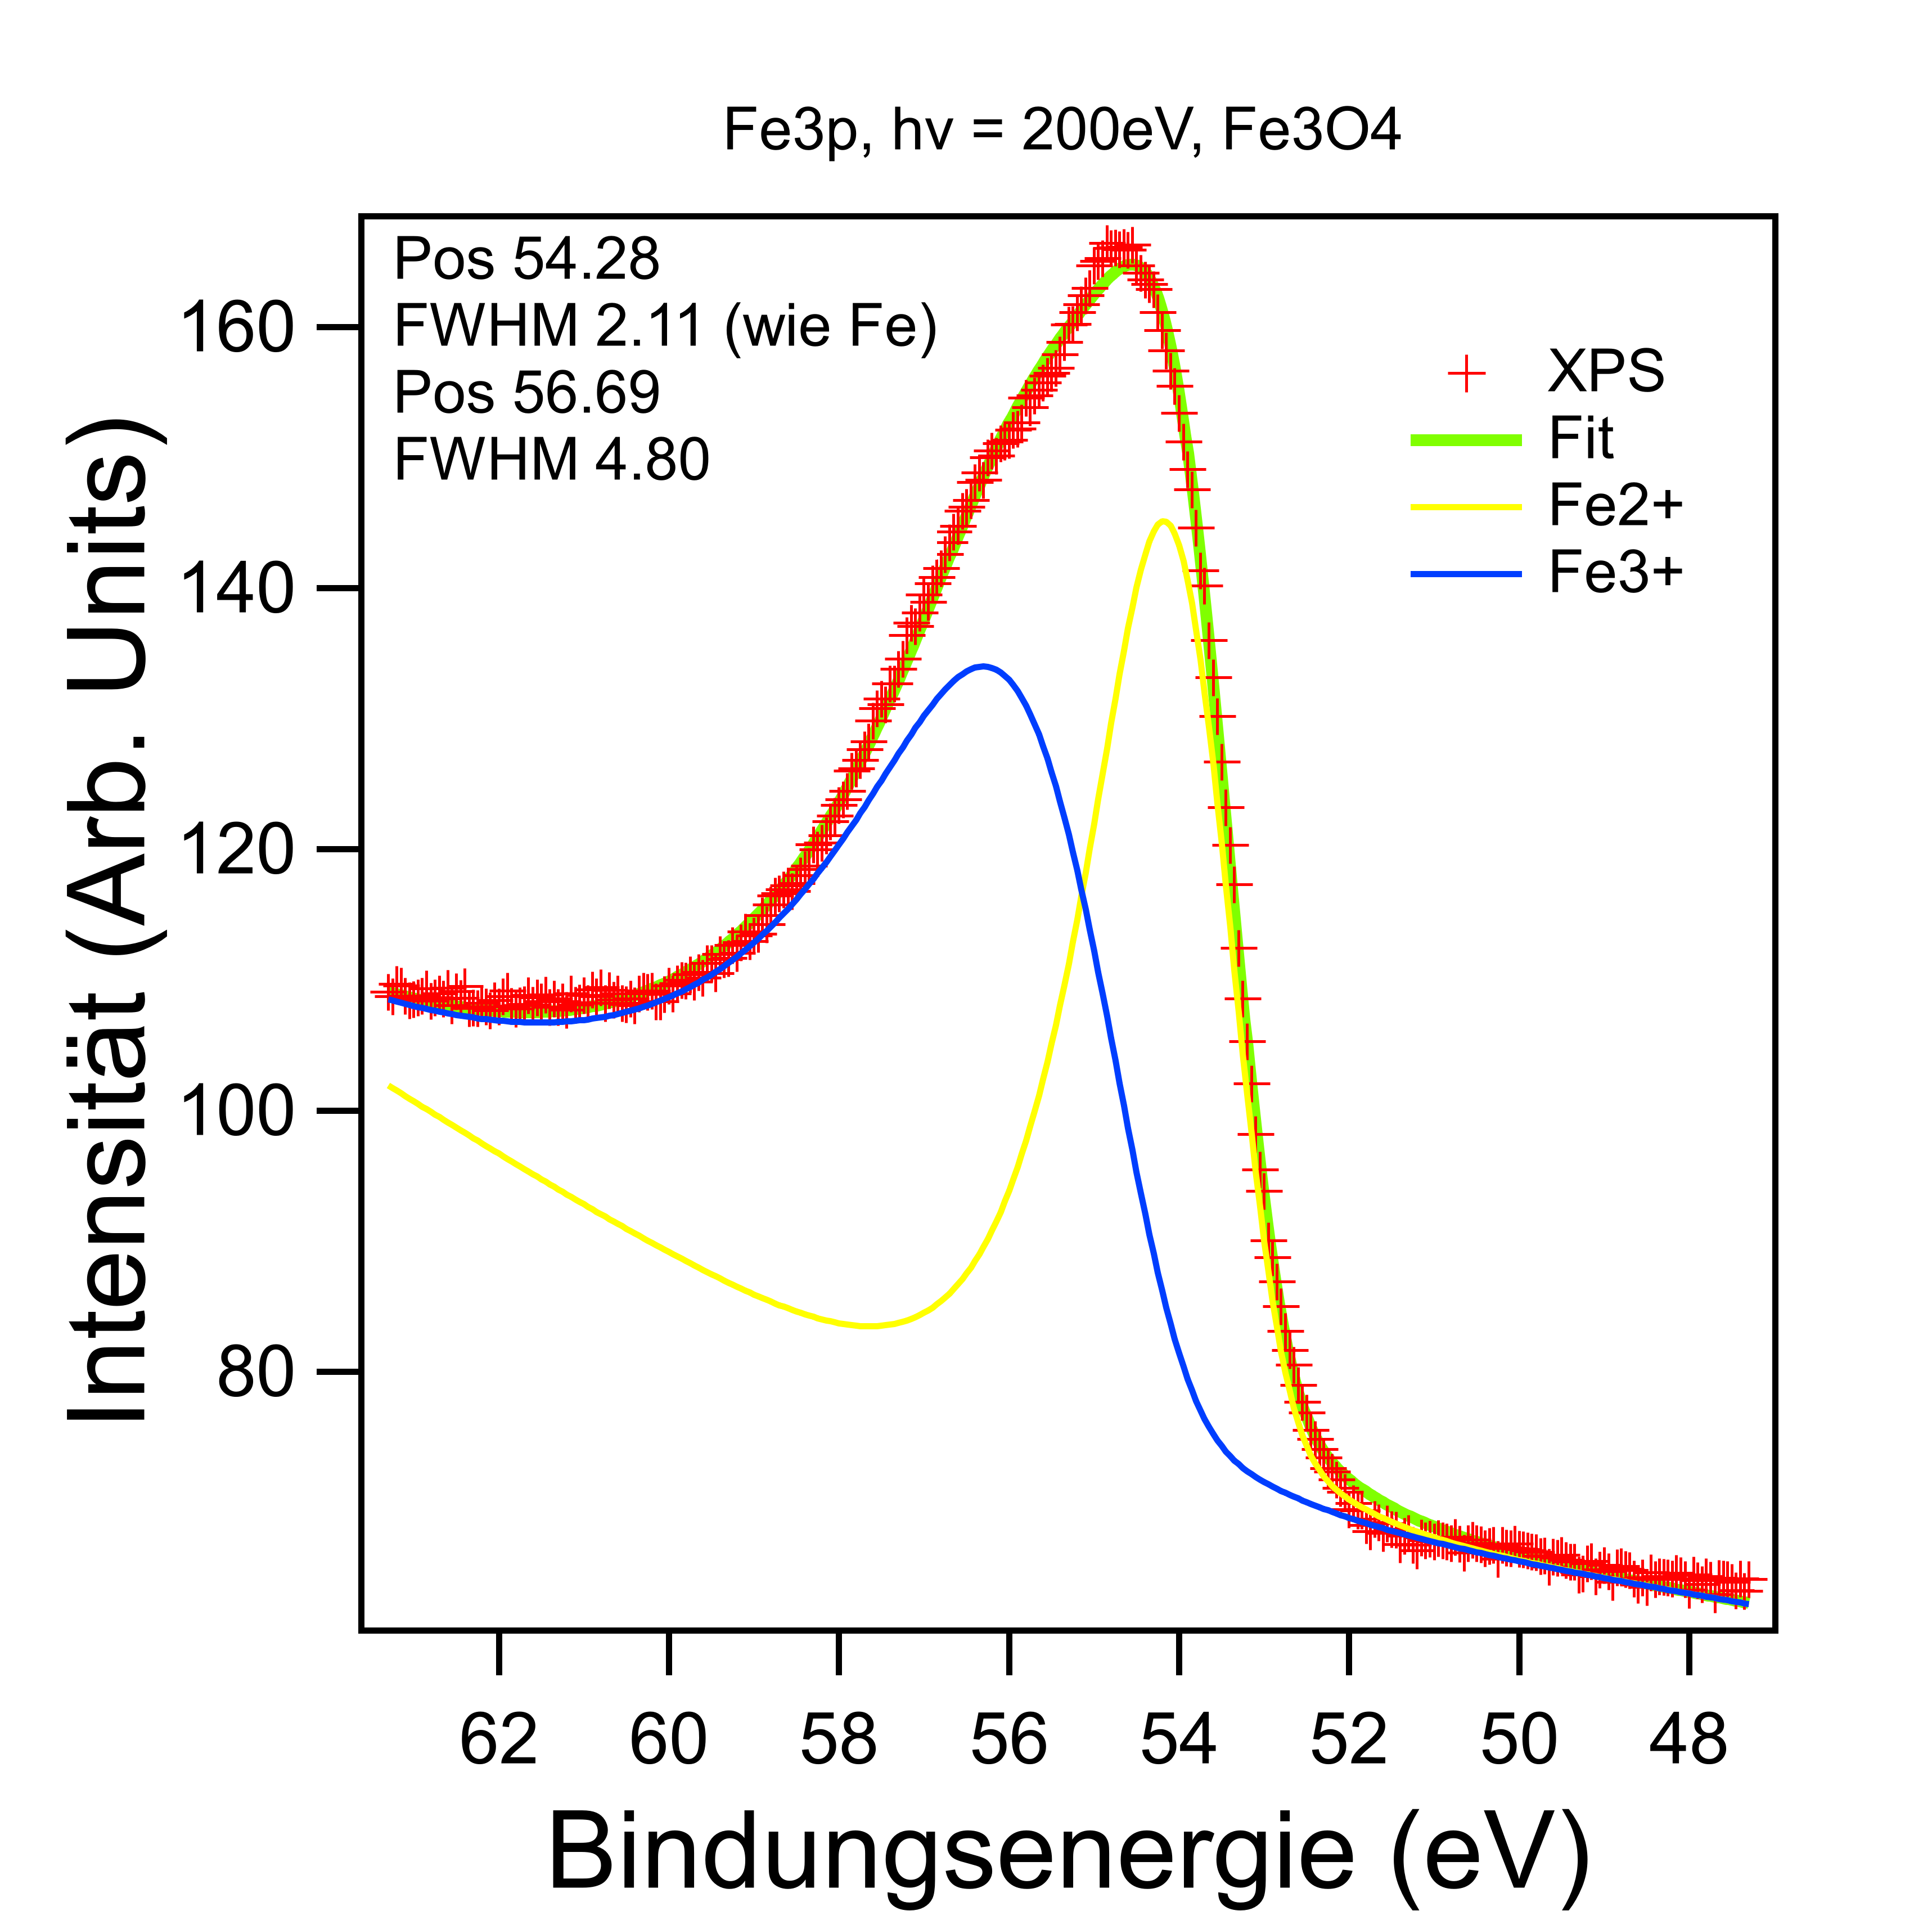
\includegraphics[height=5cm]{./content/pictures/Fe3O4/Fe3p_Fe3O4.png}
                \subcaption{Spektrum des $\ce{Fe}_{3\text{p}}$ Übergang. Gleiches Problem wie beim \ce{FeO} (s. \autoref{fig:XPSFe3p_Fe}) funktioniert abenfalls besser mit Tougaard als Shirley.}
                \label{fig:XPSFe3p_Fe3O4}
            \end{subfigure}
            \caption{Die XPS Spektren der Kernniveaus für das Magnetit.}
            \label{fig:XPS_Fe3O4}
        \end{figure}

        Um genauer zu überprüfen wird auch die chemisch sensetive Methode der Röntgenphotoelektronenspektroskopie angewendet.
        Die entsprechenden Spektren des $\ce{O}_{1\text{s}}$ Signals, sowie des $\ce{Fe}_{3\text{p}}$ Signals sind in \autoref{fig:XPS_Fe3O4} dargstellt.

        Mit Hilfe des magnetischen Röntgen-Zirkular-Dikorismus und magnetischen Röntgen-Linear-Dikorismus lassen sich die magnetischen Eigeschaften des Substrates untersuchen.
        Beide Spektren der Röntgenabsorptionsmessungen sind in \autoref{fig:XAS_Fe3O4} zu sehen.

        Wie bereits schon bei dem Nickeloxid brachte das Aufdampfen von einer Monolage Pentacene keine geordnete Struktur mit sich.


    \section{Wüstit}
        \begin{figure}
            \centering
            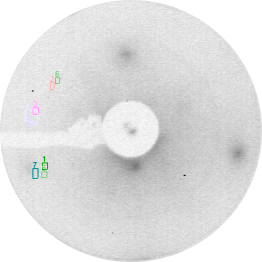
\includegraphics[height=5cm]{./content/pictures/FeO/2021_09_09_001_FeO_125eV.png}
            \caption{\ce{FeO} (100) bei einer Elektronenenergie von \SI{125}{\electronvolt}.}
            \label{fig:LEED_FeO}
        \end{figure}
        Um die Wüstitstruktur zu erhalten wird die Magnetitstruktur zunächst auf \SI{650}{\celsius} aufgeheizt.
        Anschließend werden vermehrt Sauerstoffatome durch ioneninduziertes Zerstäuben ausgelöst um so die Wüstit Zusammensetzung zu erhalten.
        Im anschluss wird die probe nochmal auf \SI{650}{\celsius} erwärmt.
        Dabei entsteht dann das LEED Bild aus \autoref{fig:LEED_FeO}.
        Die Intensitäten sind beim Eisenoxid im Gegensatz zu dem passivierten Eisen invertiert, wobei die zuvor starken Spots nicht mehr sichtbar sind.
        Trotz der gleichen Elektronenenergie von \SI{125}{\electronvolt} sind die Spots leicht nach außen gewandert.
        Dies Widerspricht sich mit der eigentlich größeren Gitterkonstante von Eisenoxid im Bezug auf die $\text{p}(1 \times 1)\ce{O}$ Überstruktur des passivierten Eisens.

        \begin{figure}
            \centering
            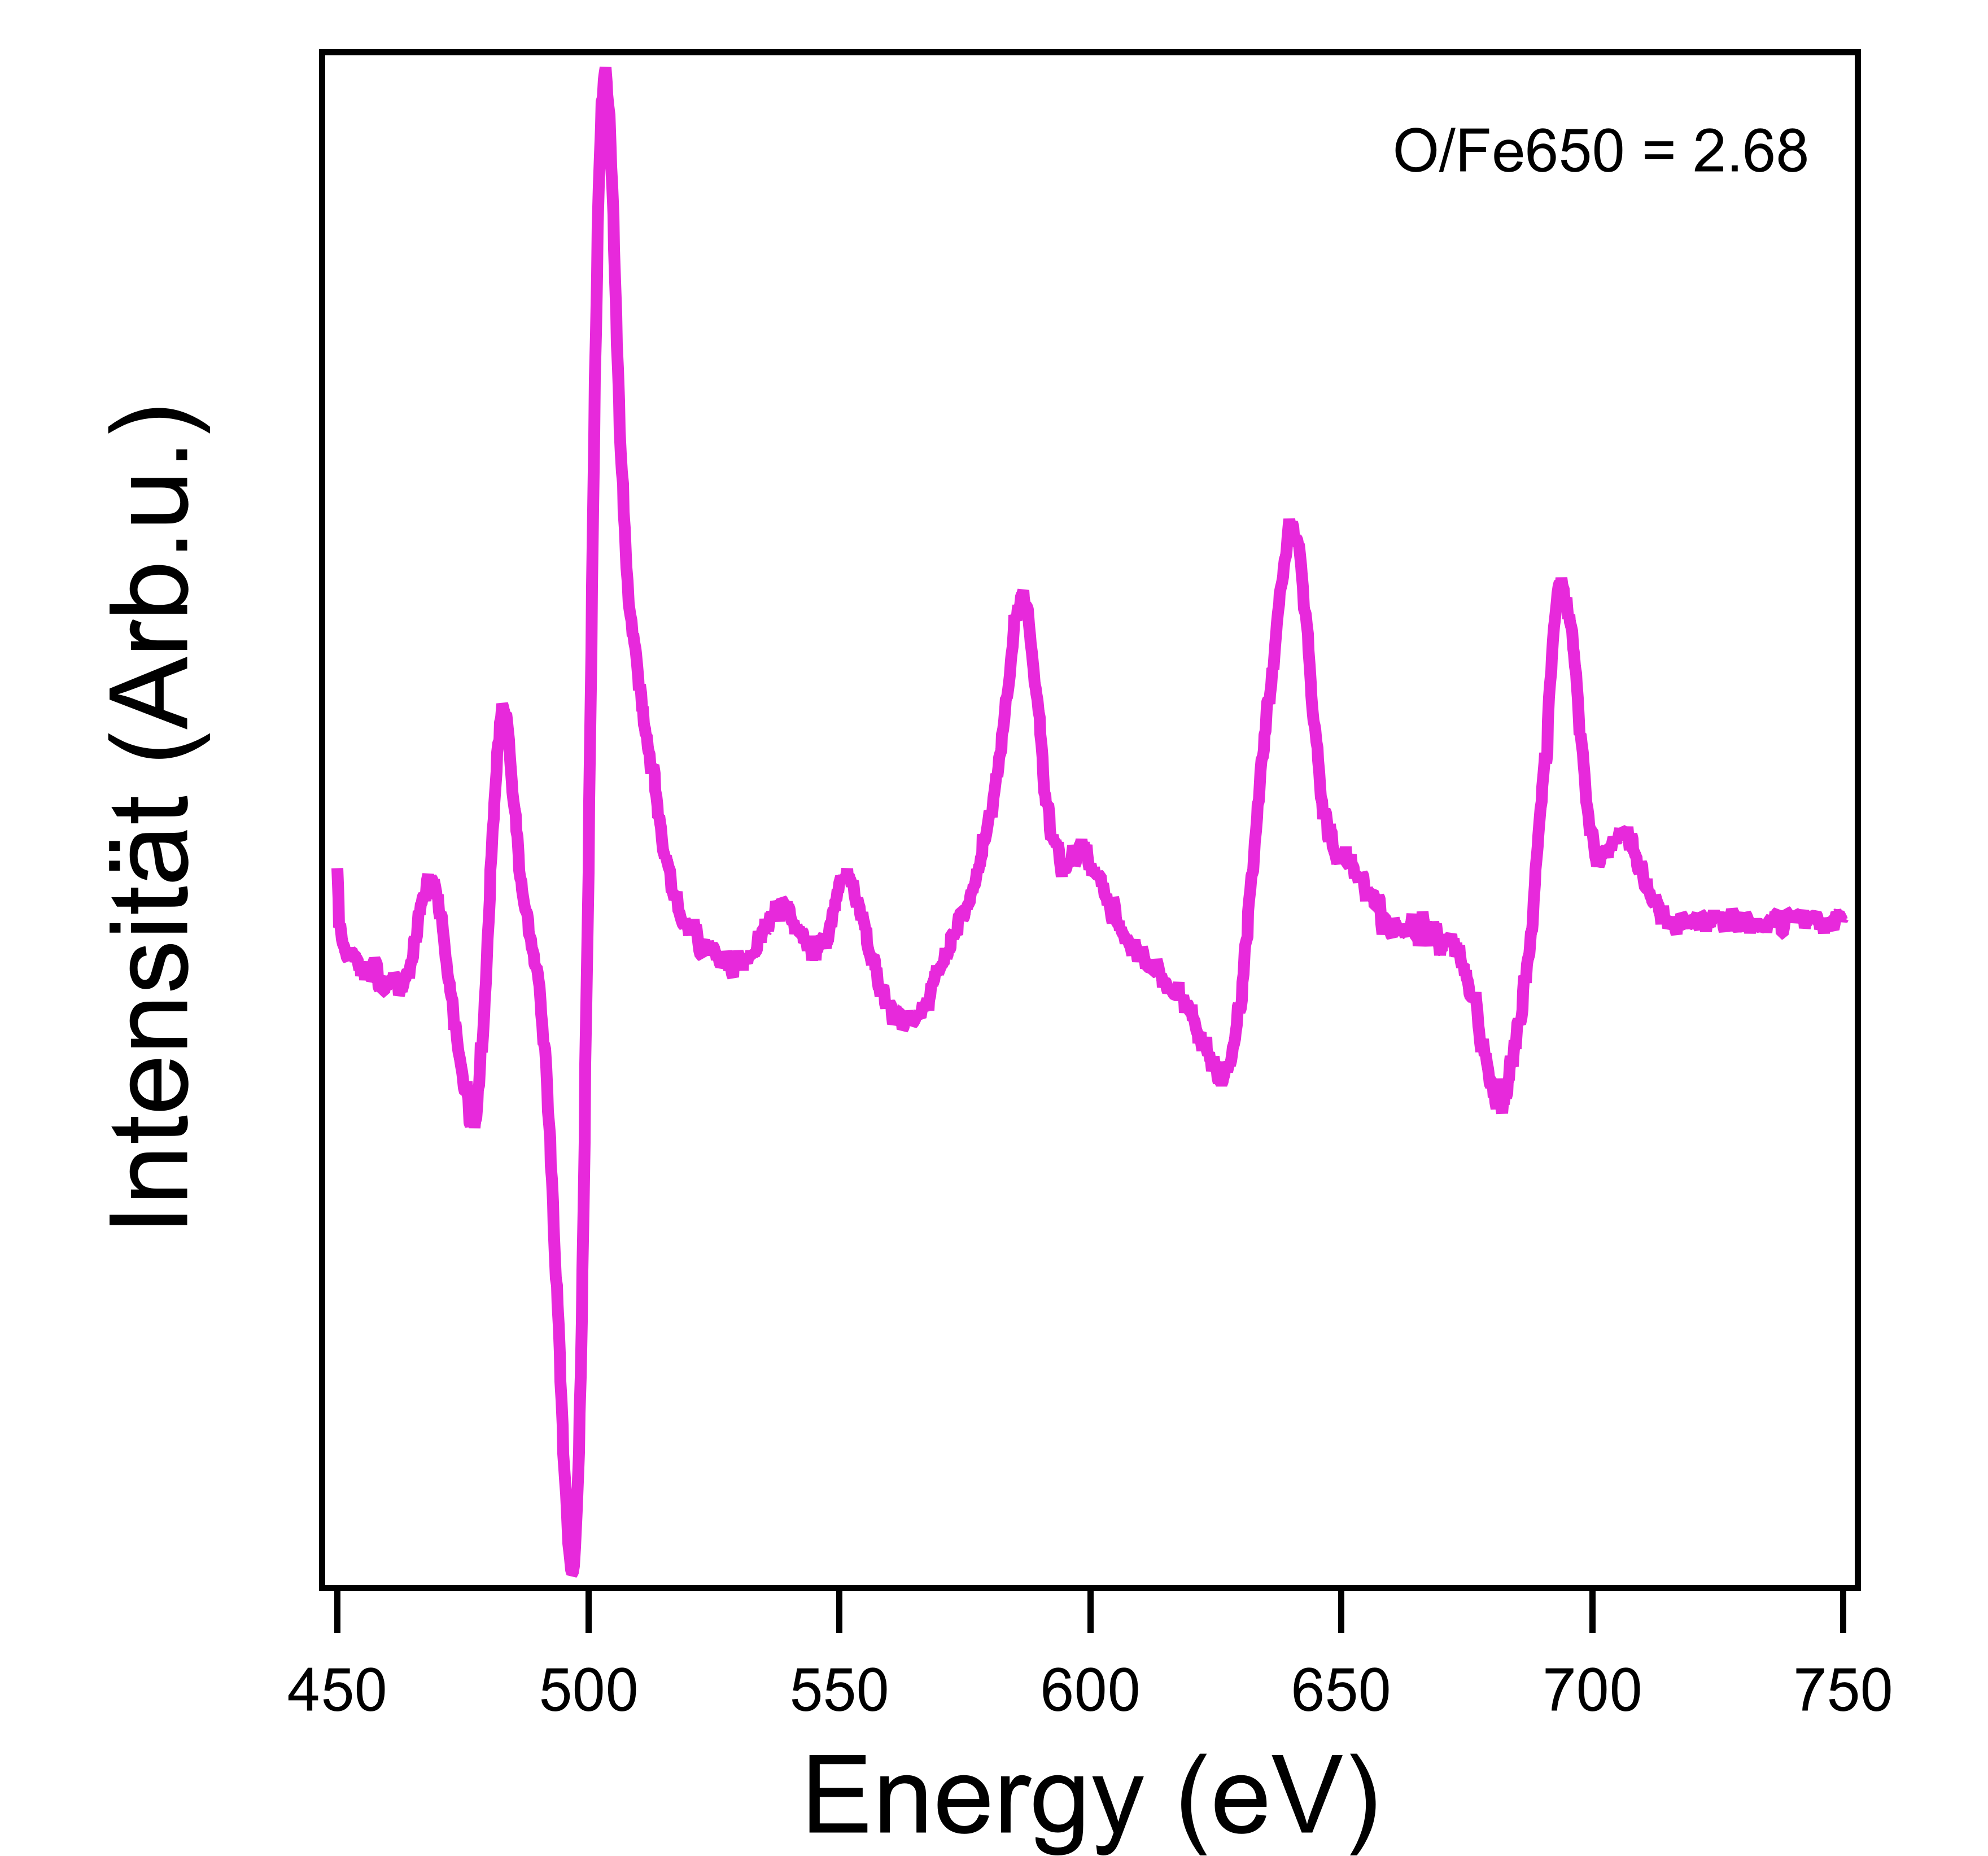
\includegraphics[height=5cm]{./content/pictures/FeO/AES_FeO.png}
            \caption{Das Augerspektrum der Wüstitprobe.}
            \label{fig:Auger_FeO}
        \end{figure}
        \begin{figure}
            \centering
            \begin{subfigure}[t]{0.48\textwidth}
                \centering
                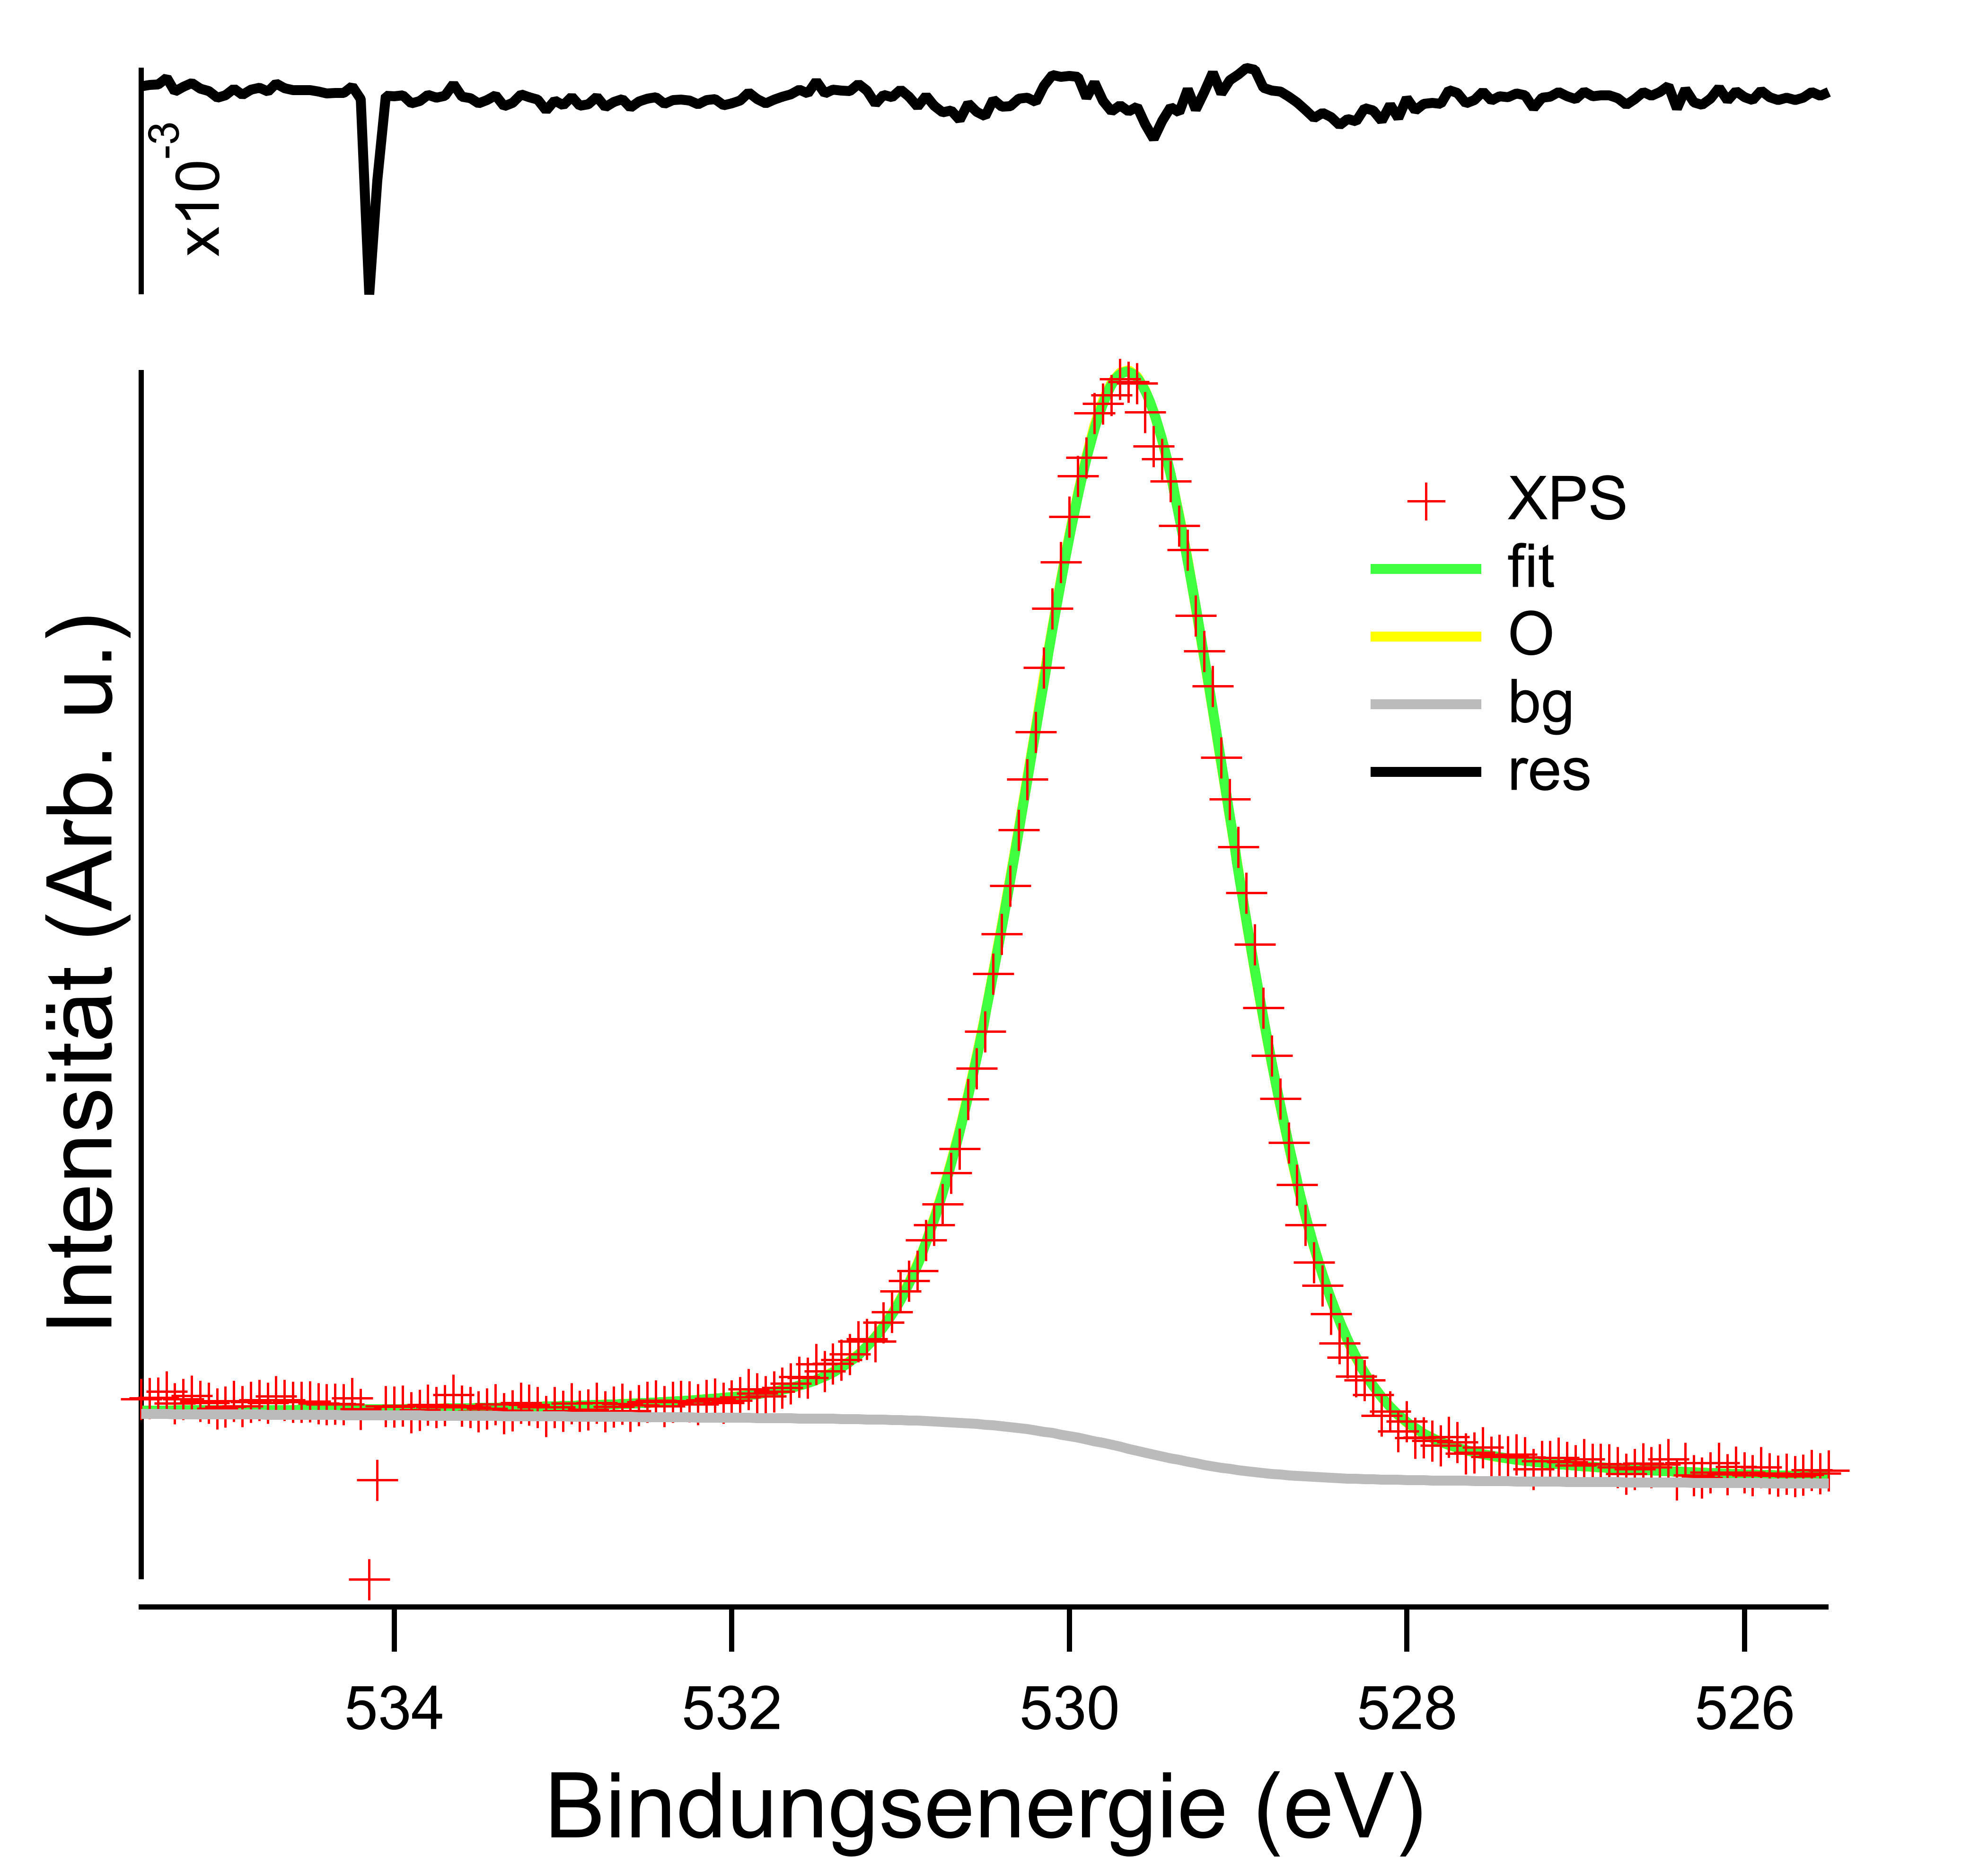
\includegraphics[height=5cm]{./content/pictures/FeO/O1s_FeO.png}
                \subcaption{Spektrum des $\ce{O}_{1\text{s}}$ Übergang. Fit mit einem Peak (kleiner Shirley) sehr gut.}
                \label{fig:XPSO1s_FeO}
            \end{subfigure}
            \begin{subfigure}[t]{0.48\textwidth}
                \centering
                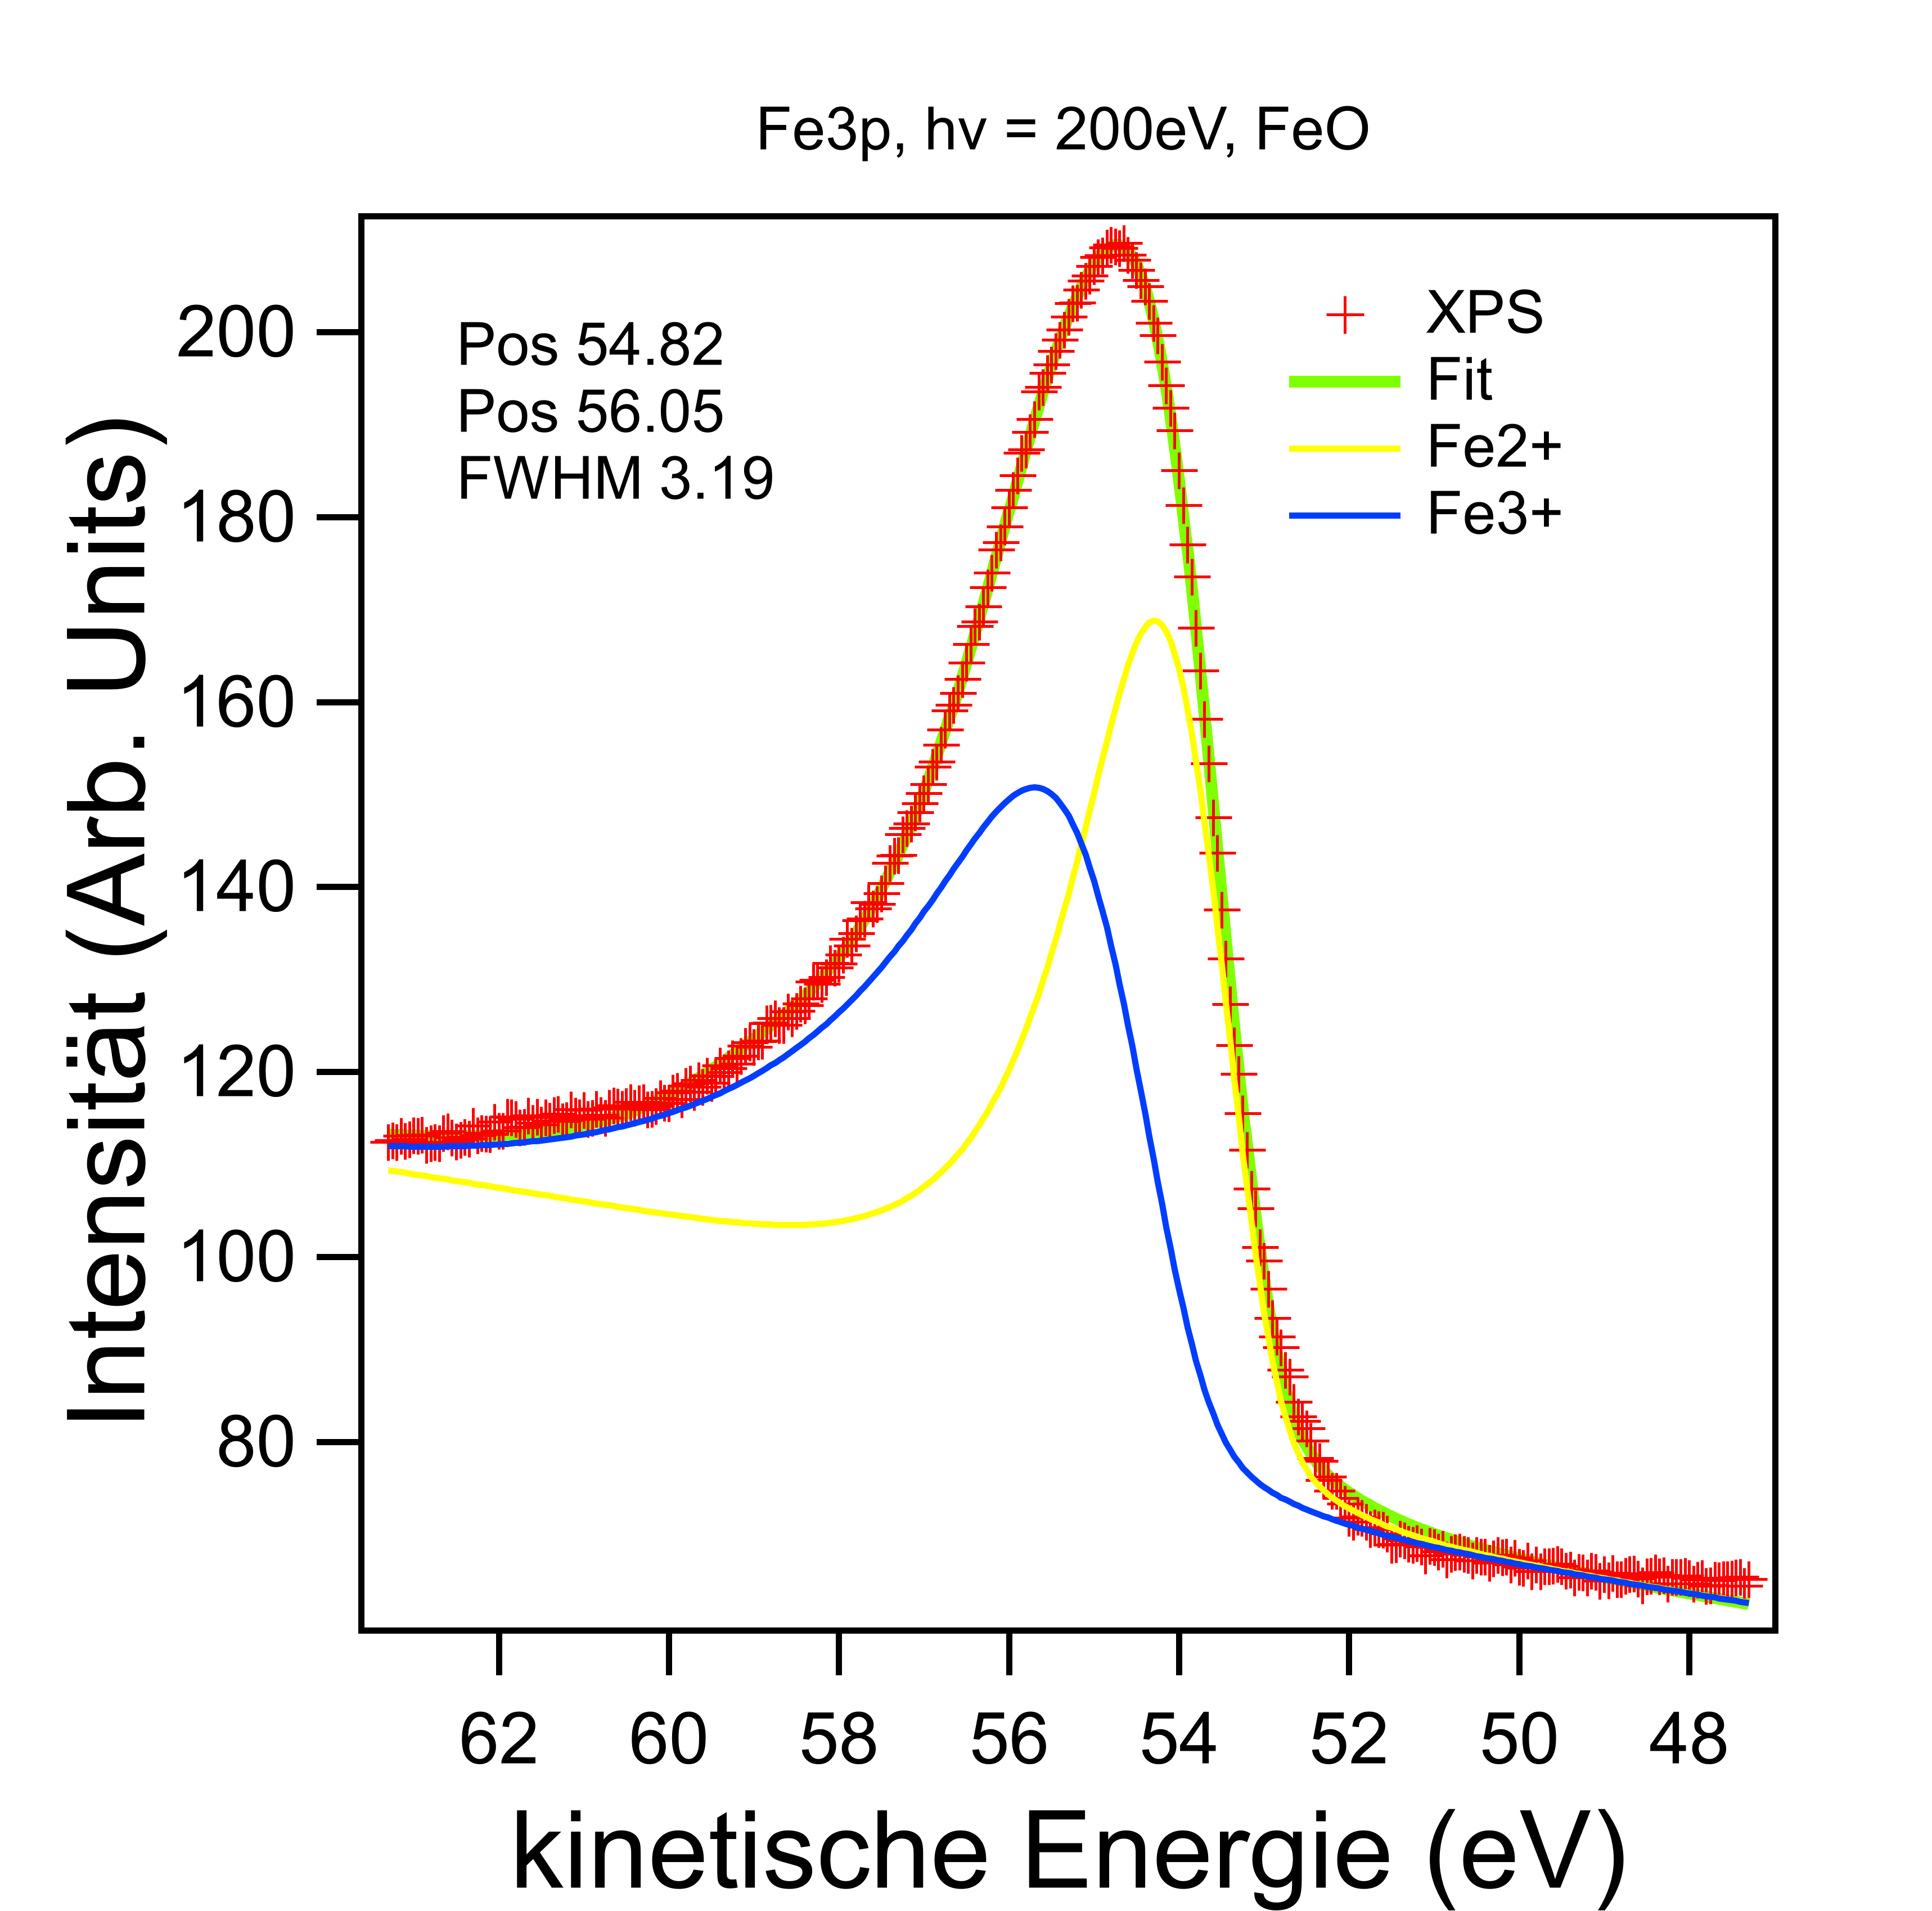
\includegraphics[height=5cm]{./content/pictures/FeO/Fe3p_FeO.png}
                \subcaption{Spektrum des $\ce{Fe}_{3\text{p}}$ Übergang. Zuornung sehr schwierig, ein großer Peak bei kleinen BE und ein kleiner bei großen BE passen. Aber auch zwei etwa gleichgroße Peaks. Je nach dem wie die Parameter gewählt und festgestzt werden.}
                \label{fig:XPSFe3p_FeO}
            \end{subfigure}
            \caption{}
            \label{fig:XPS_FeO}
        \end{figure}
        Das Verhältnis aus Sauerstoff und Eisen kann dabei erneut mittels Augerelektronenspektroskopie überprüft werden.
        Auch das Augerspektrum in \autoref{fig:Auger_FeO} mit dem bereits von Carpa u.A. \cite{FeO_1} entdecken Augerelektronenspektrum für Eisenoxid zeigt gute Übereinstimmung.
        Ebenfalls deutet das Peakverhältnis von dem Sauerstoffsignal und Eisen mit \num{2.53} auf $\ce{FeO}$ hin, da dies nur leicht unterhalb des Wertes aus der Literatur von \num{2.89} liegt \cite{FeO_1}.
        Einen genaueren Einblick welche Struktur vorliegt kann erneut die Röntgenphotoelektronenspektroskopie bieten.
        Die entsprechenden Spektren sind in \autoref{fig:XPS_FeO} zu finden.

        \begin{figure}
            \centering
            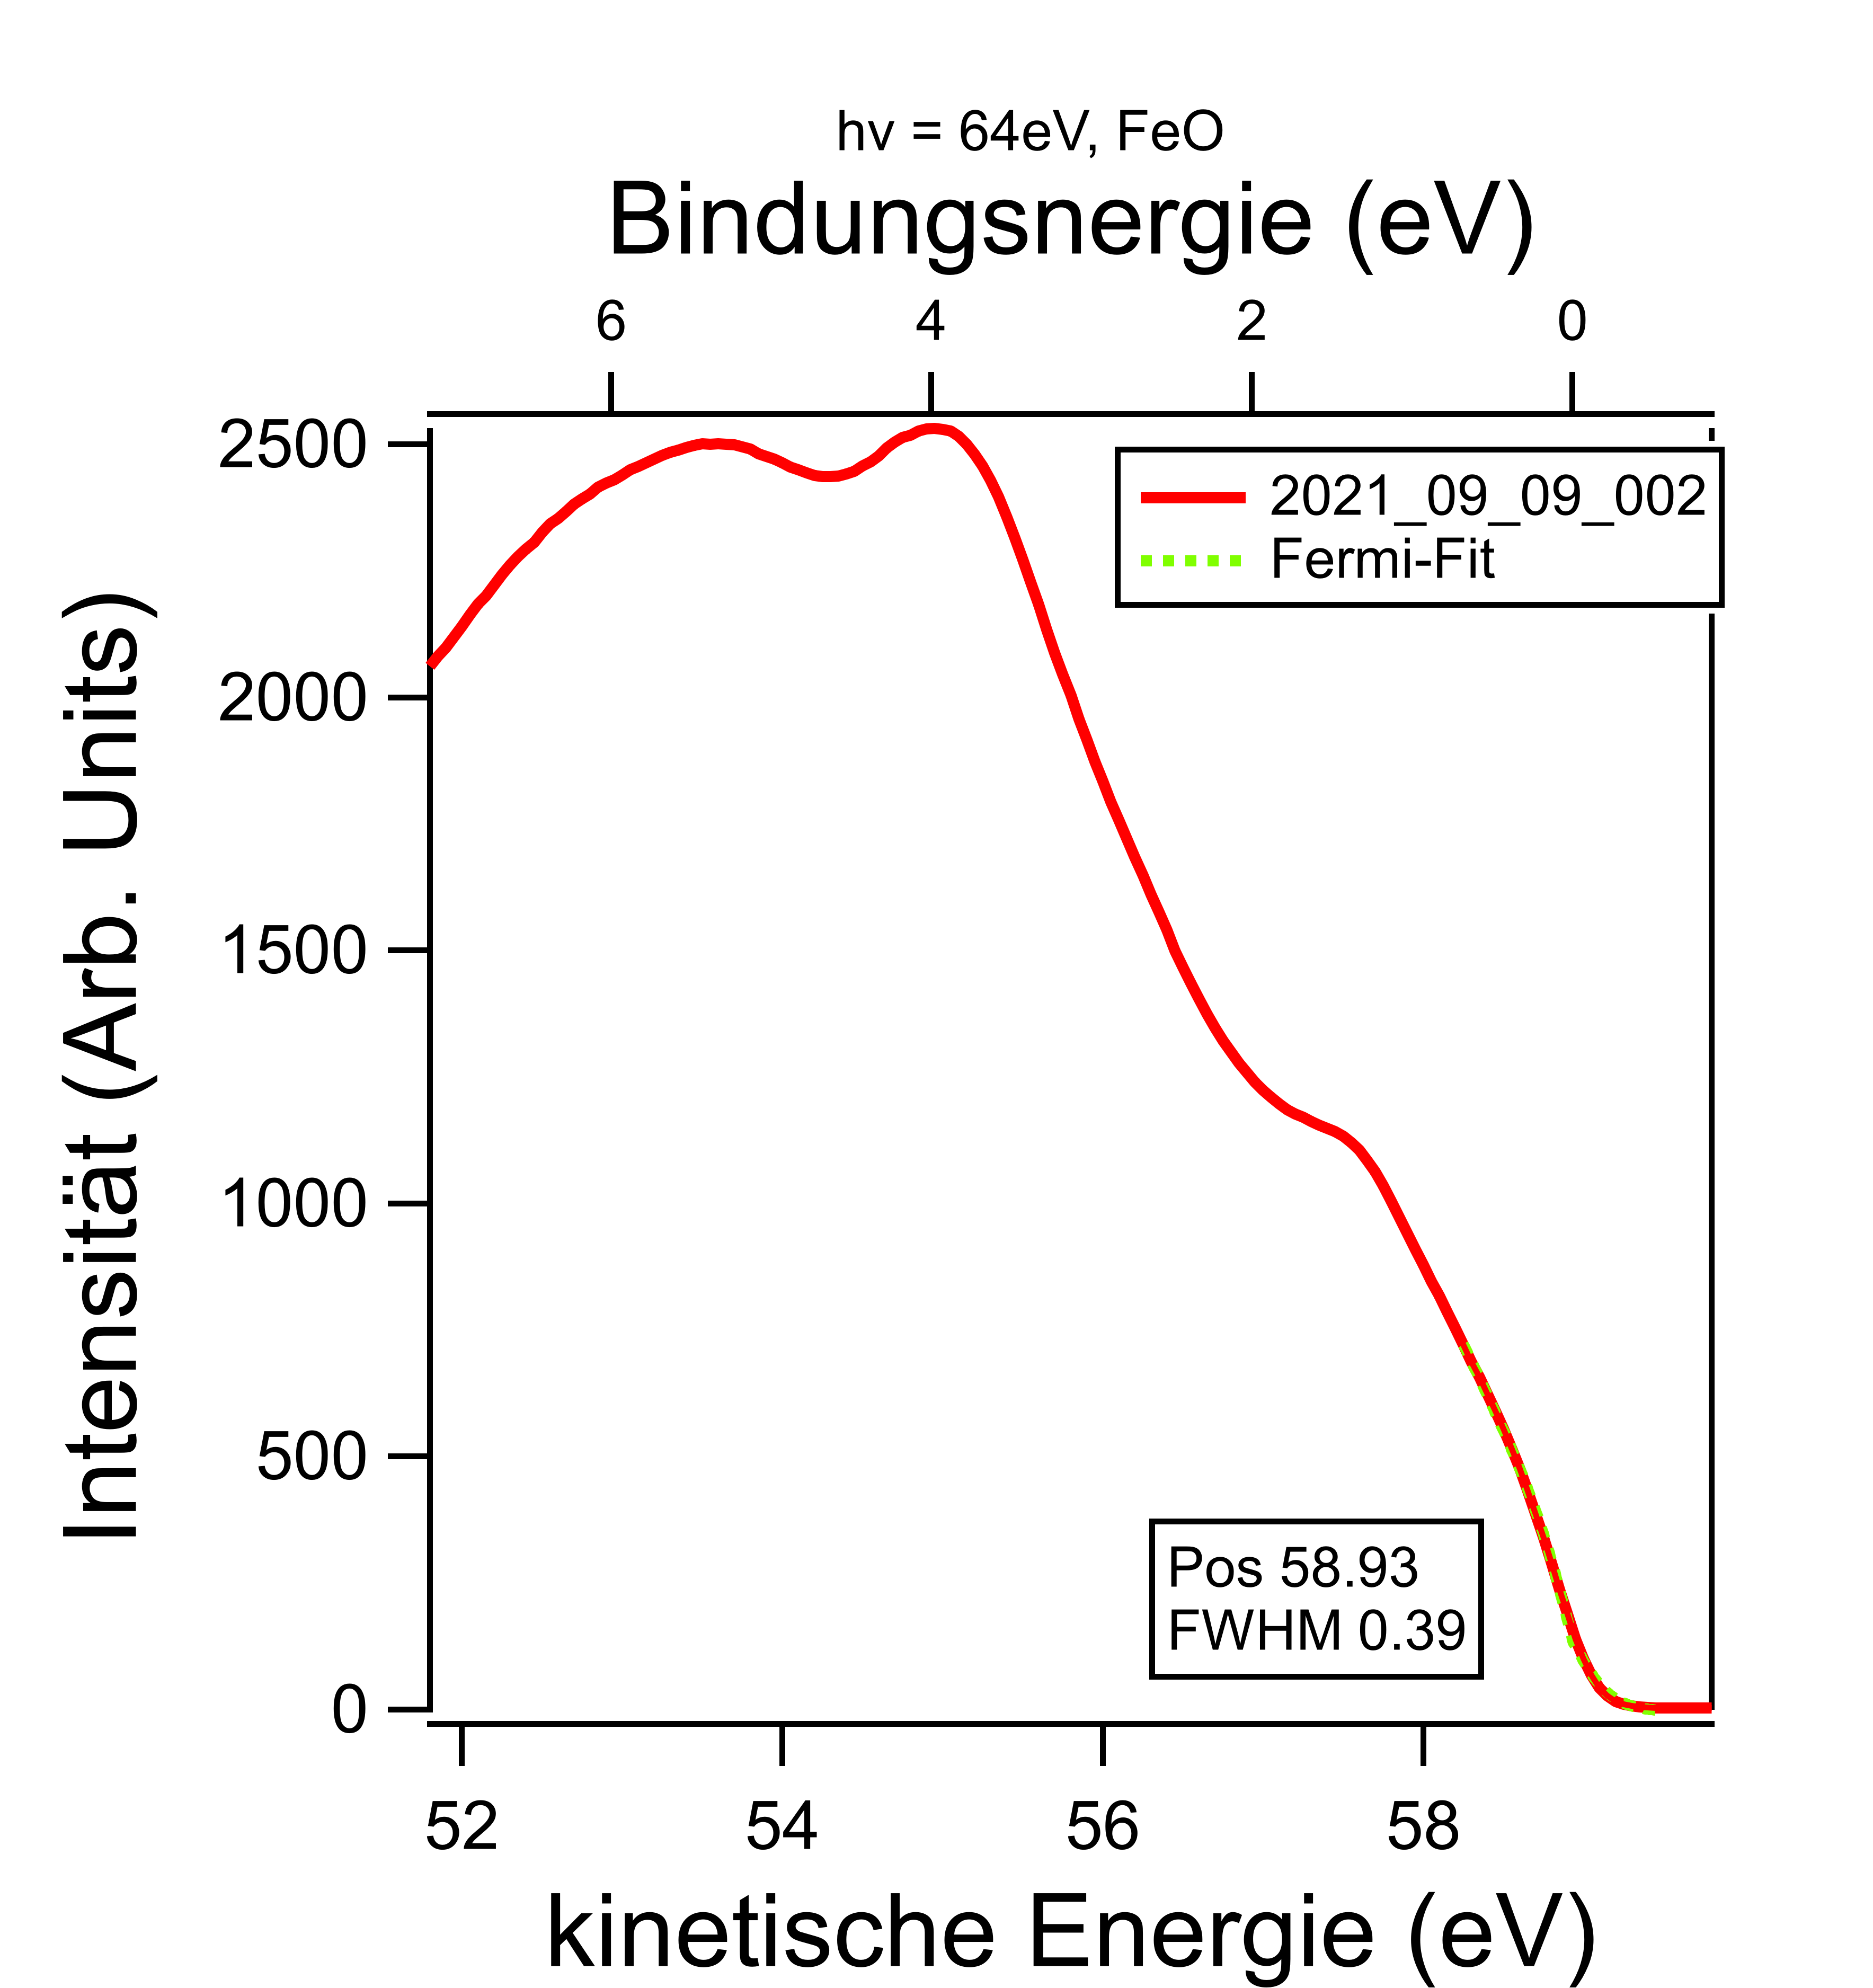
\includegraphics[width=0.5\textwidth]{./content/pictures/FeO/Fermi_FeO.png}
            \caption{Valenzbandspektrum der des \ce{FeO} bei einer Photonenenergie von \SI{64}{\electronvolt}. Zusätzlich eingetragen ist der Fit der Fermikante.}
            \label{fig:EDC_FeO}
        \end{figure}
        Ebenso ist in \autoref{fig:EDC_FeO} die Elektronendichtekurve für den Valenzbandbereich des \ce{FeO} aufgetragen.

        \begin{figure}
            \centering
            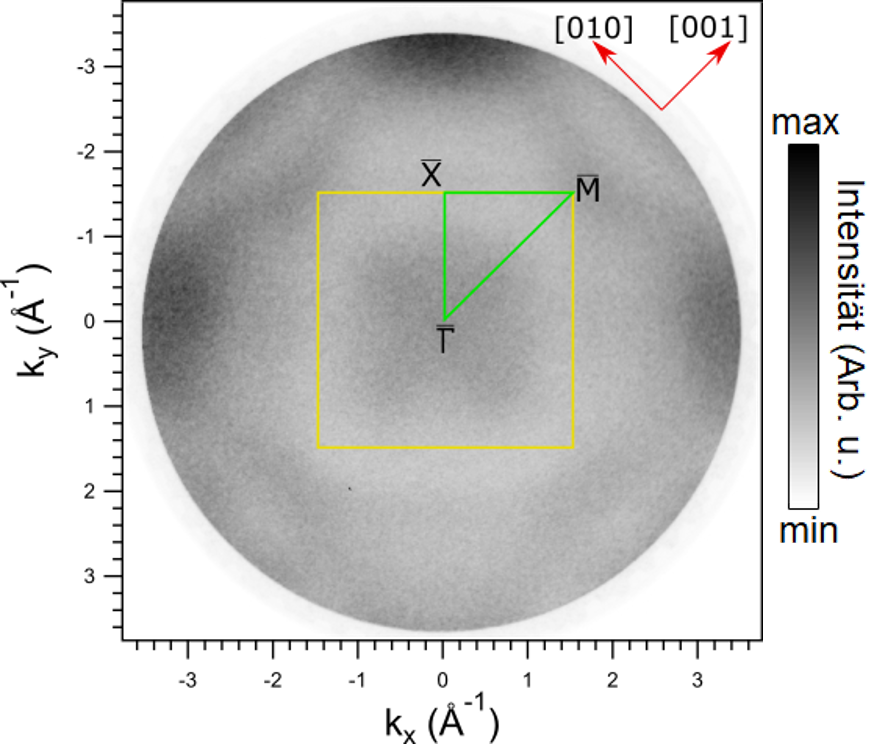
\includegraphics[width=0.5\textwidth]{./content/pictures/FeO/BZ_FeO.png}
            \caption{Die Brillouinzone des Eisensoxid bei einer Bindungsenergie von \SI{1.95}{\electronvolt}.
            Eigezeichnet sind auch die Vektoren, sowie einige Hochsymmetrierichtungen.
            Die Kantenlänge der BZ ist $\frac{2\pi}{a}\sqrt{2} = \SI[per-mode=reciprocal]{2.89}{\per\angstrom}$.
            Im Zentrum liegt der $\overline{\Gamma}$-Punkt, der Abstand zum $\overline{X}$-Punkt ist $\frac{2\pi}{2 \cdot a}\sqrt{2} = \SI[per-mode=reciprocal]{1.45}{\per\angstrom}$ und zum $\overline{M}$-Punkt $\frac{2\pi}{a} = \SI[per-mode=reciprocal]{2.05}{\per\angstrom}$ \cite{Hüfner}.
            \textbf{Problem with px-> k, WKF was Driffting up and down}}
            \label{fig:BZ_FeO}
        \end{figure}
        Auch für das Wüstit lässt sich die Oberflächenbrillouinzone definieren, die in \autoref{fig:BZ_FeO} abgebildet ist.
        ferner auch die Bandstruktur

        \begin{figure}
            \centering
            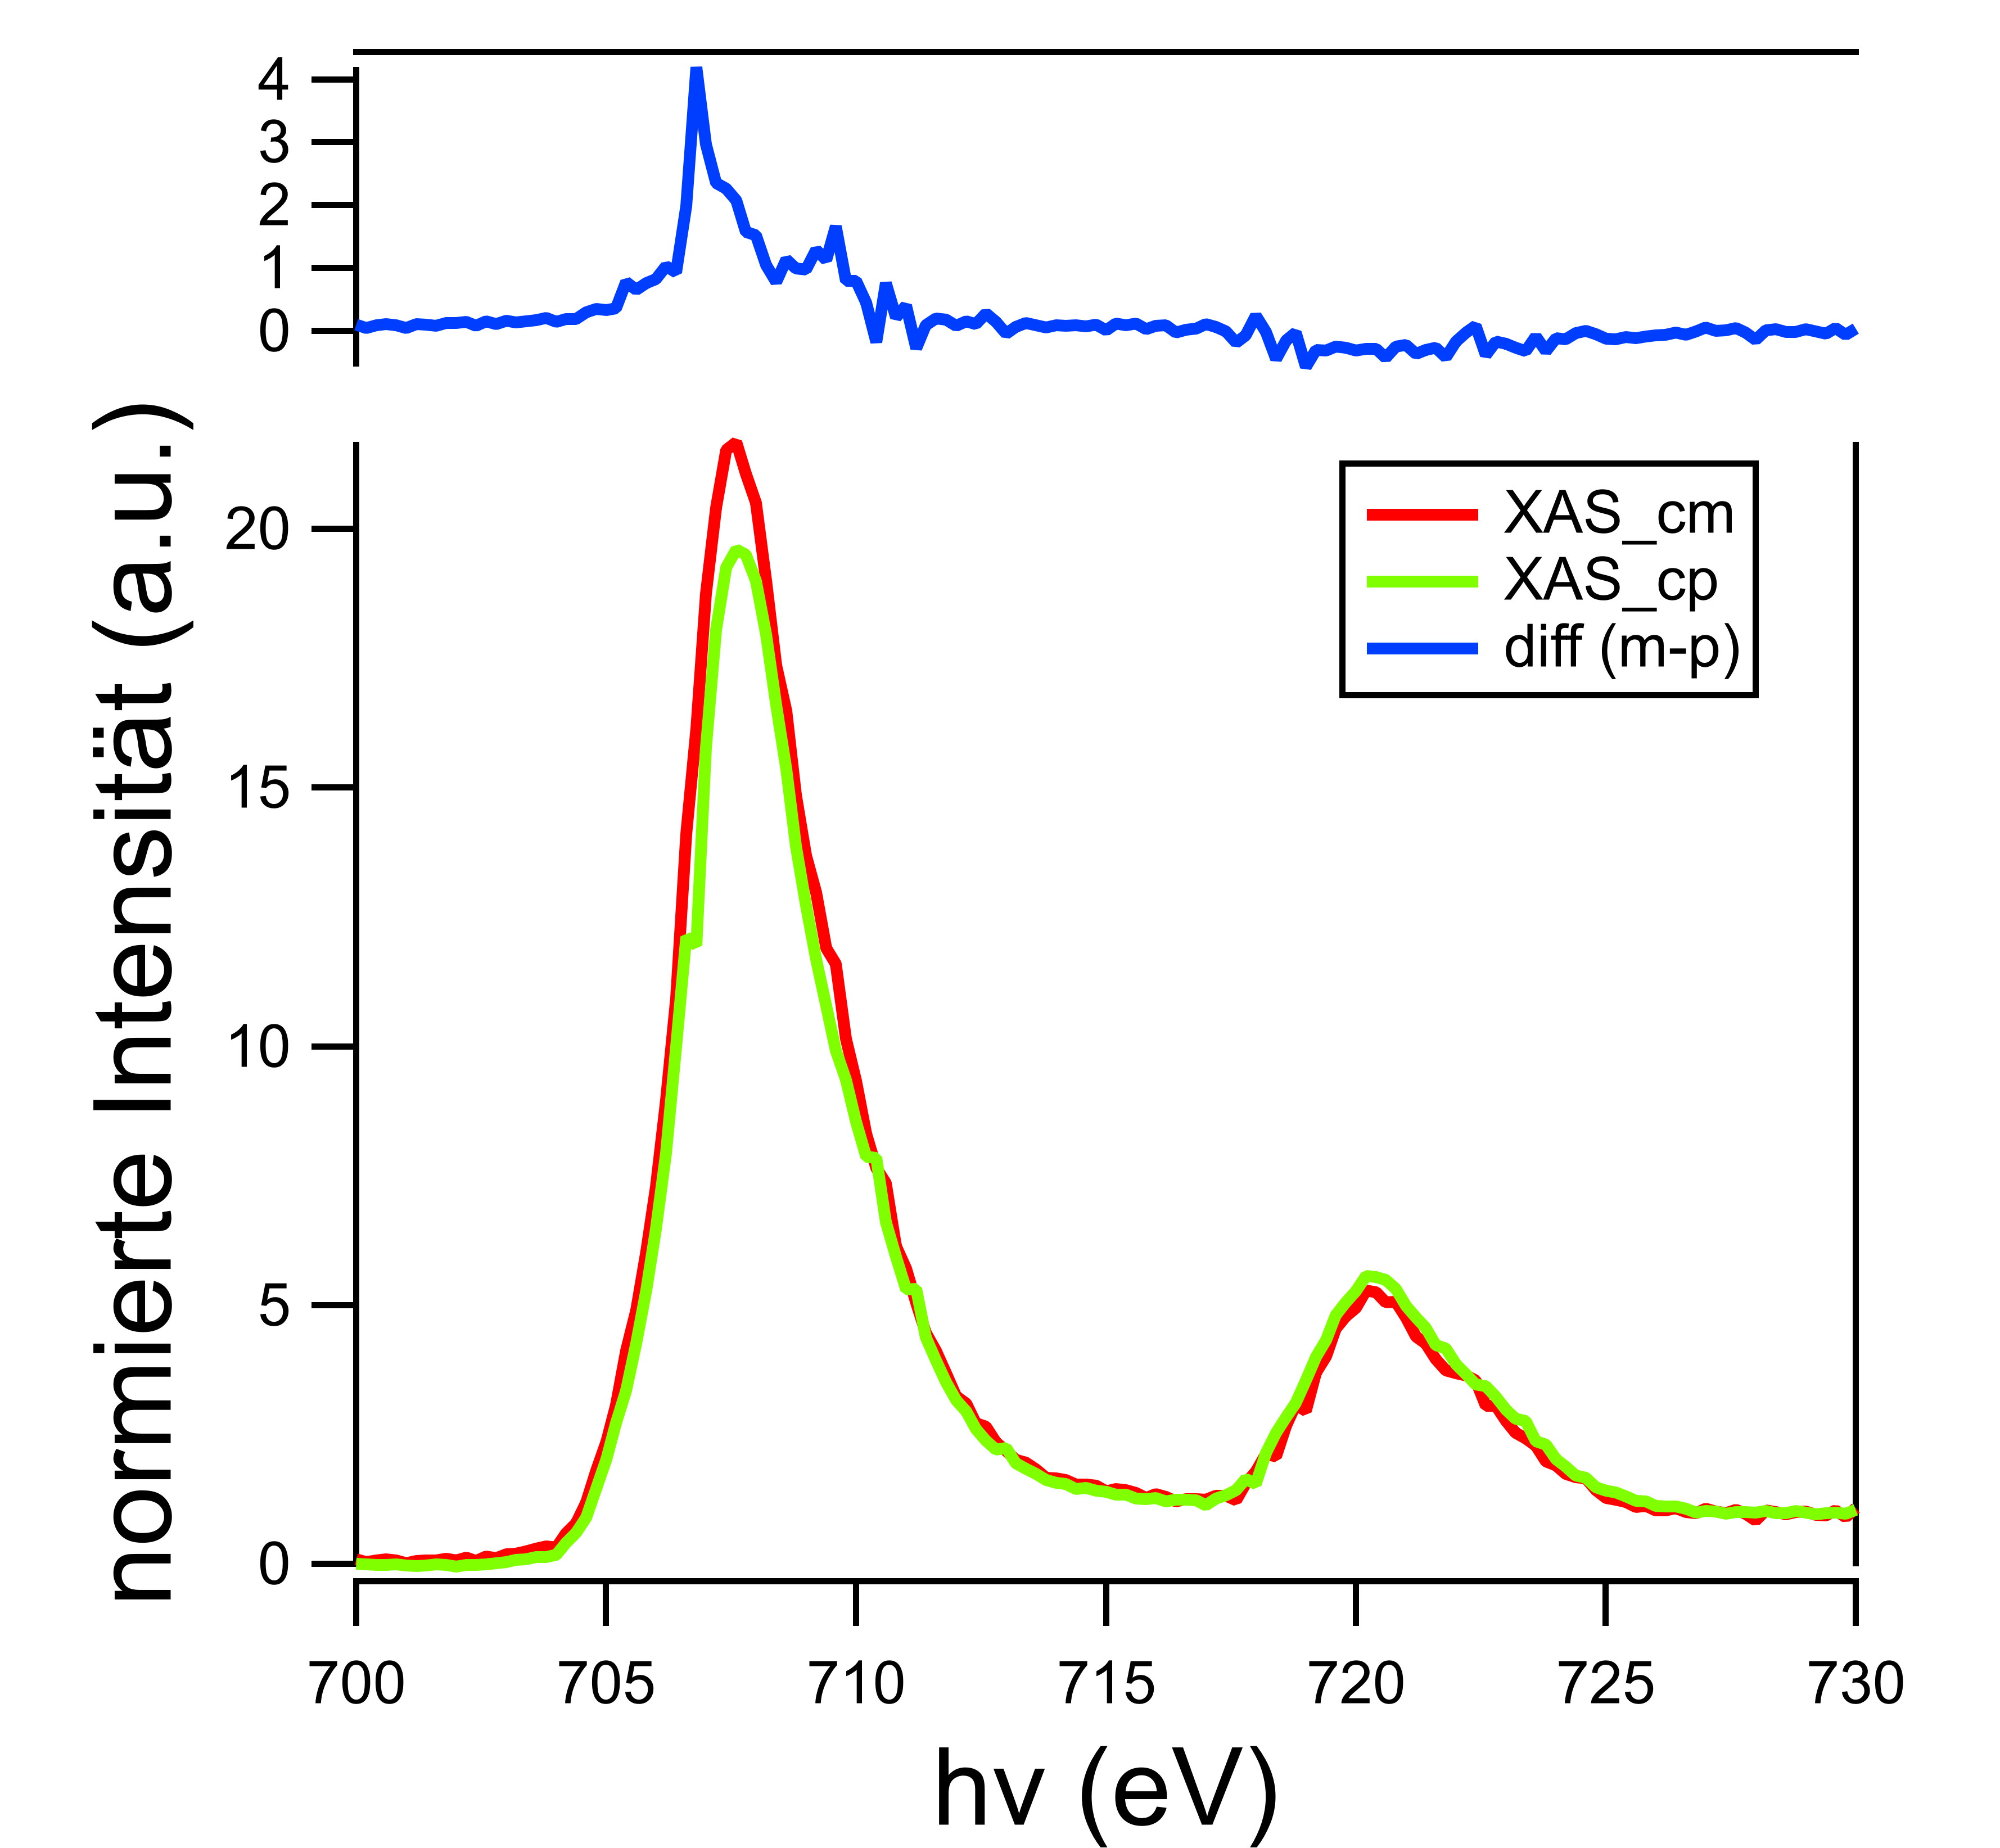
\includegraphics[height=5cm]{./content/pictures/FeO/XMCD_FeO.png}
            \caption{XAS Spektren für links- und rechtzirkular polarisiertes Licht und ihre Differenz. XMCD}
            \label{fig:XMCD}
        \end{figure}
        \begin{figure}
            \centering
            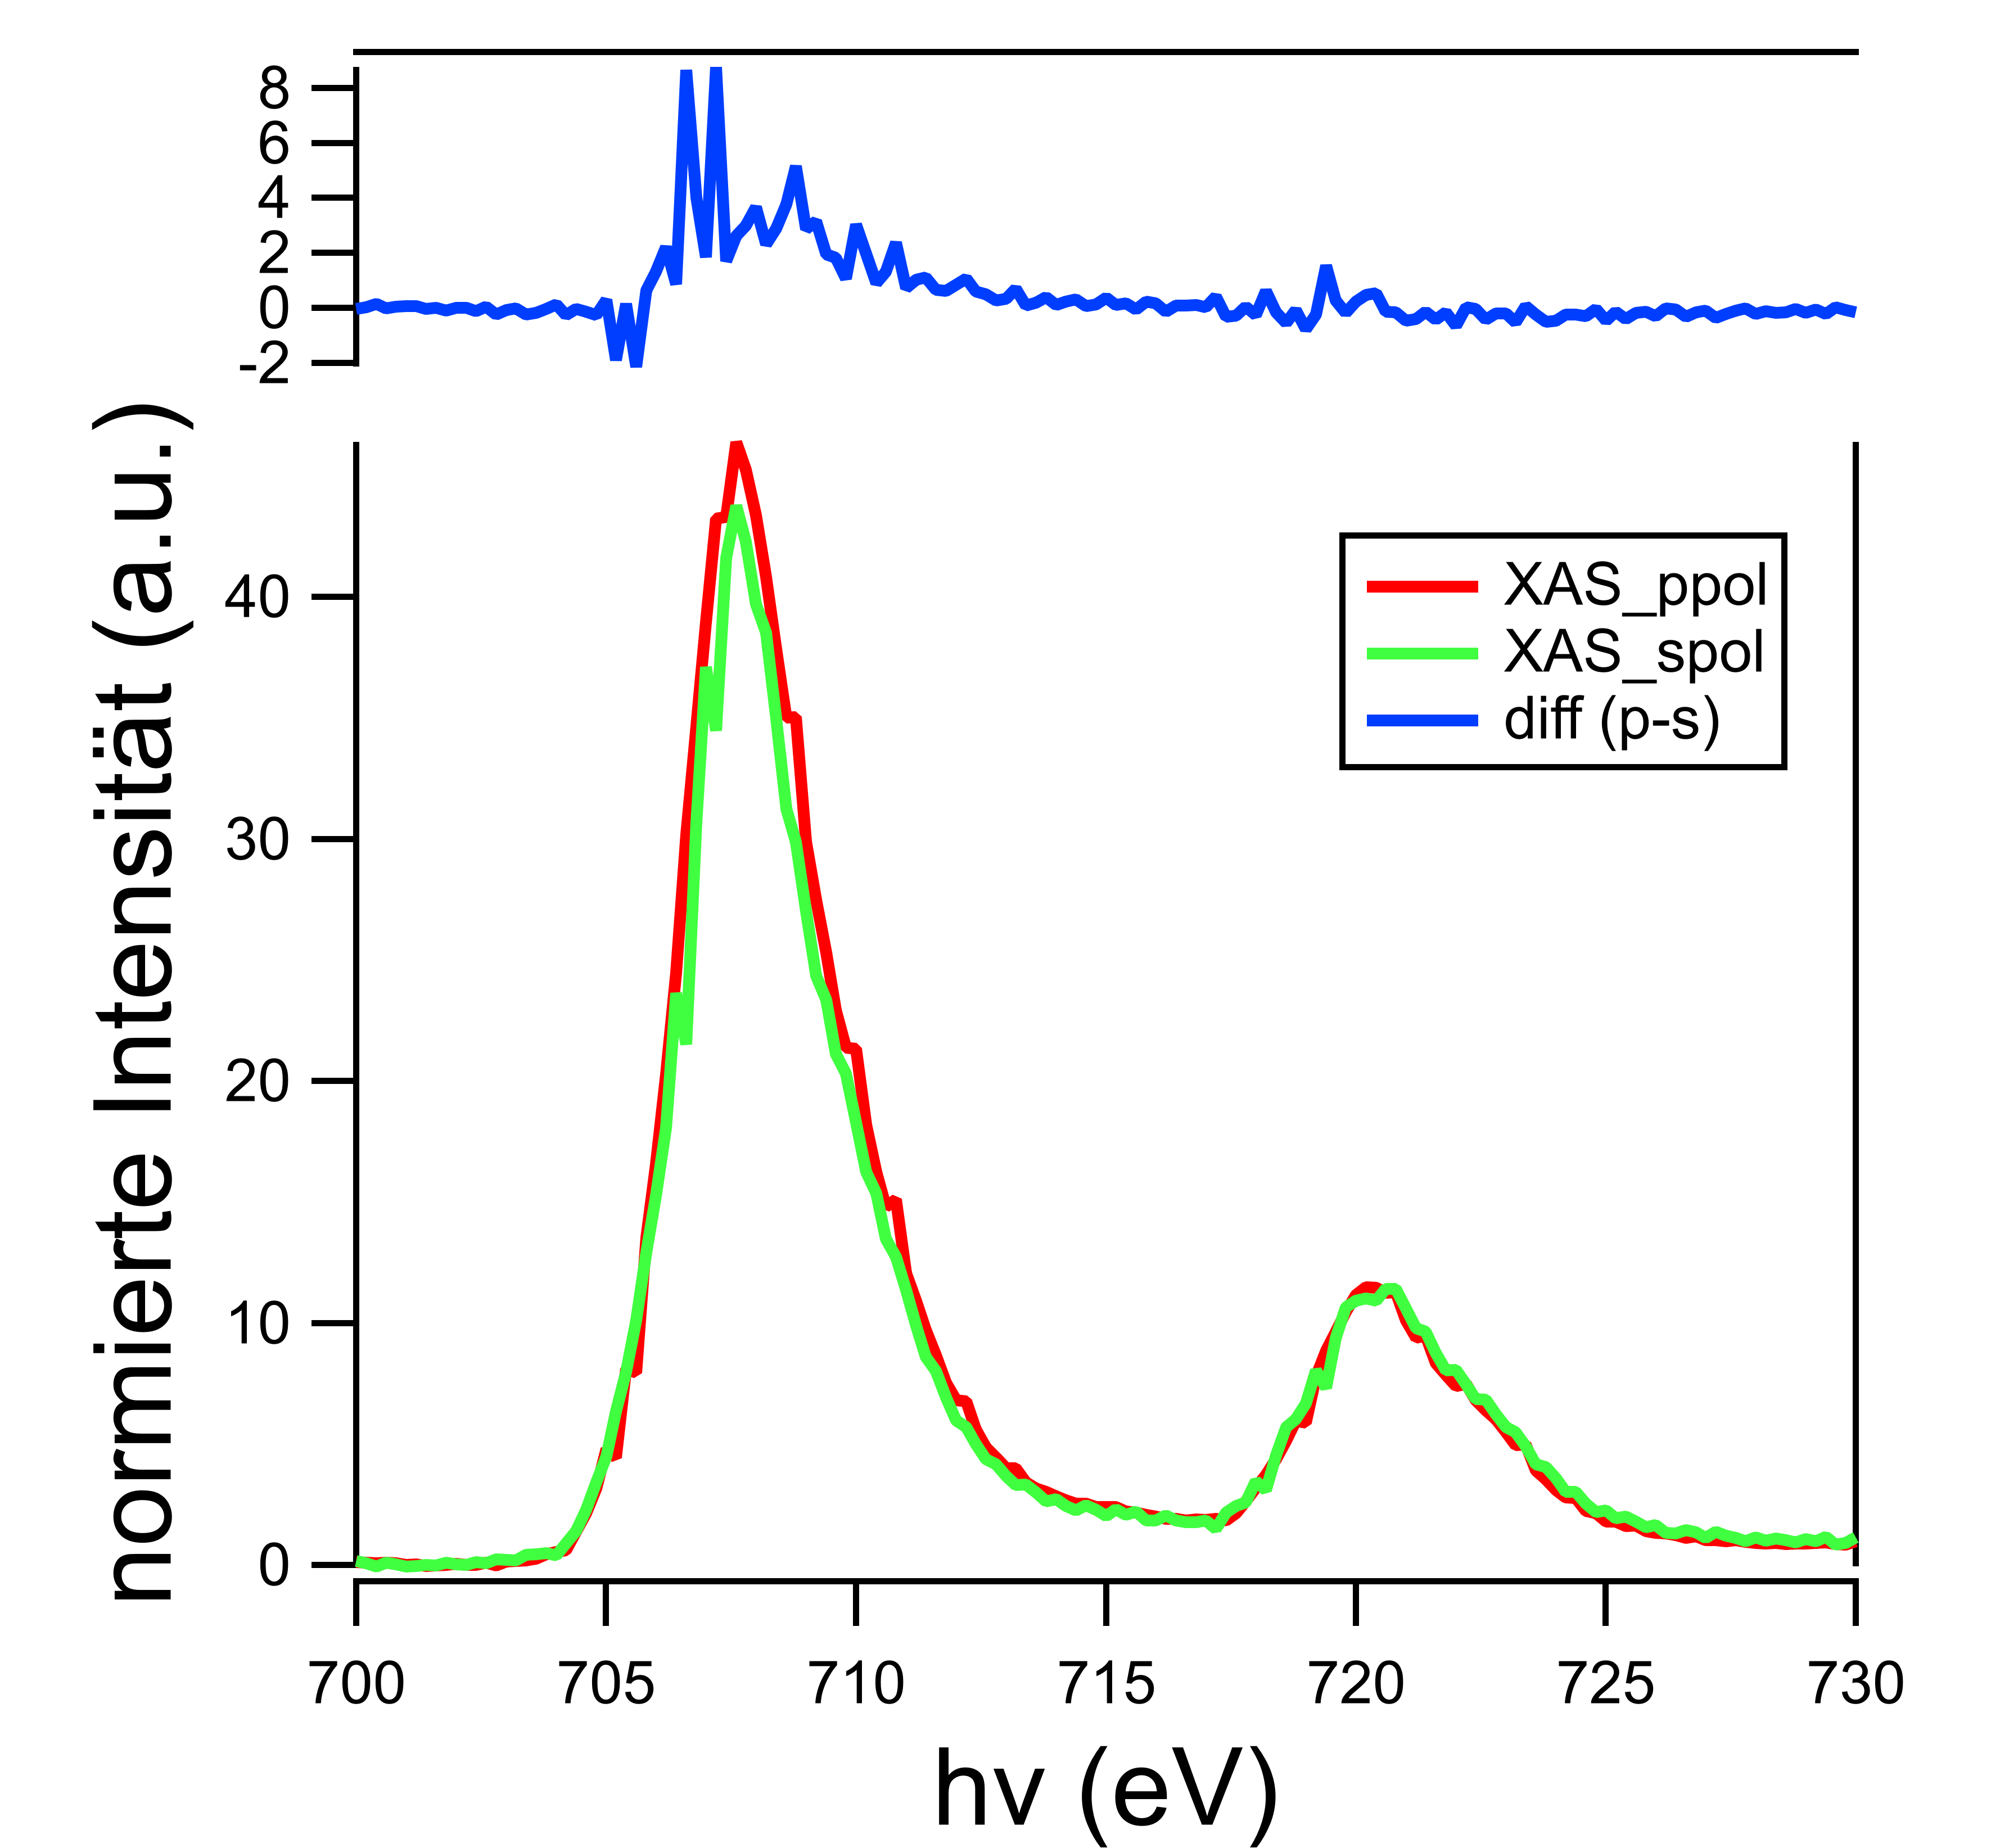
\includegraphics[height=5cm]{./content/pictures/FeO/XMLD_FeO.png}
            \caption{XAS Spektren für s- und p- polarisiertes Licht, sowie dessen Differenz. XMLD}
            \label{fig:XMLD}
        \end{figure}
        Um sich erneut die magnetischen Eigenschaften des Substrat anzuschauen werden Röntgenabsorptionsmessungen durchgeführt.
        In \autoref{fig:XAS_FeO} sind die entsprechende Spektren dargestellt.
        
        \begin{figure}
            \centering
            \begin{subfigure}[t]{0.48\textwidth}
                \centering
                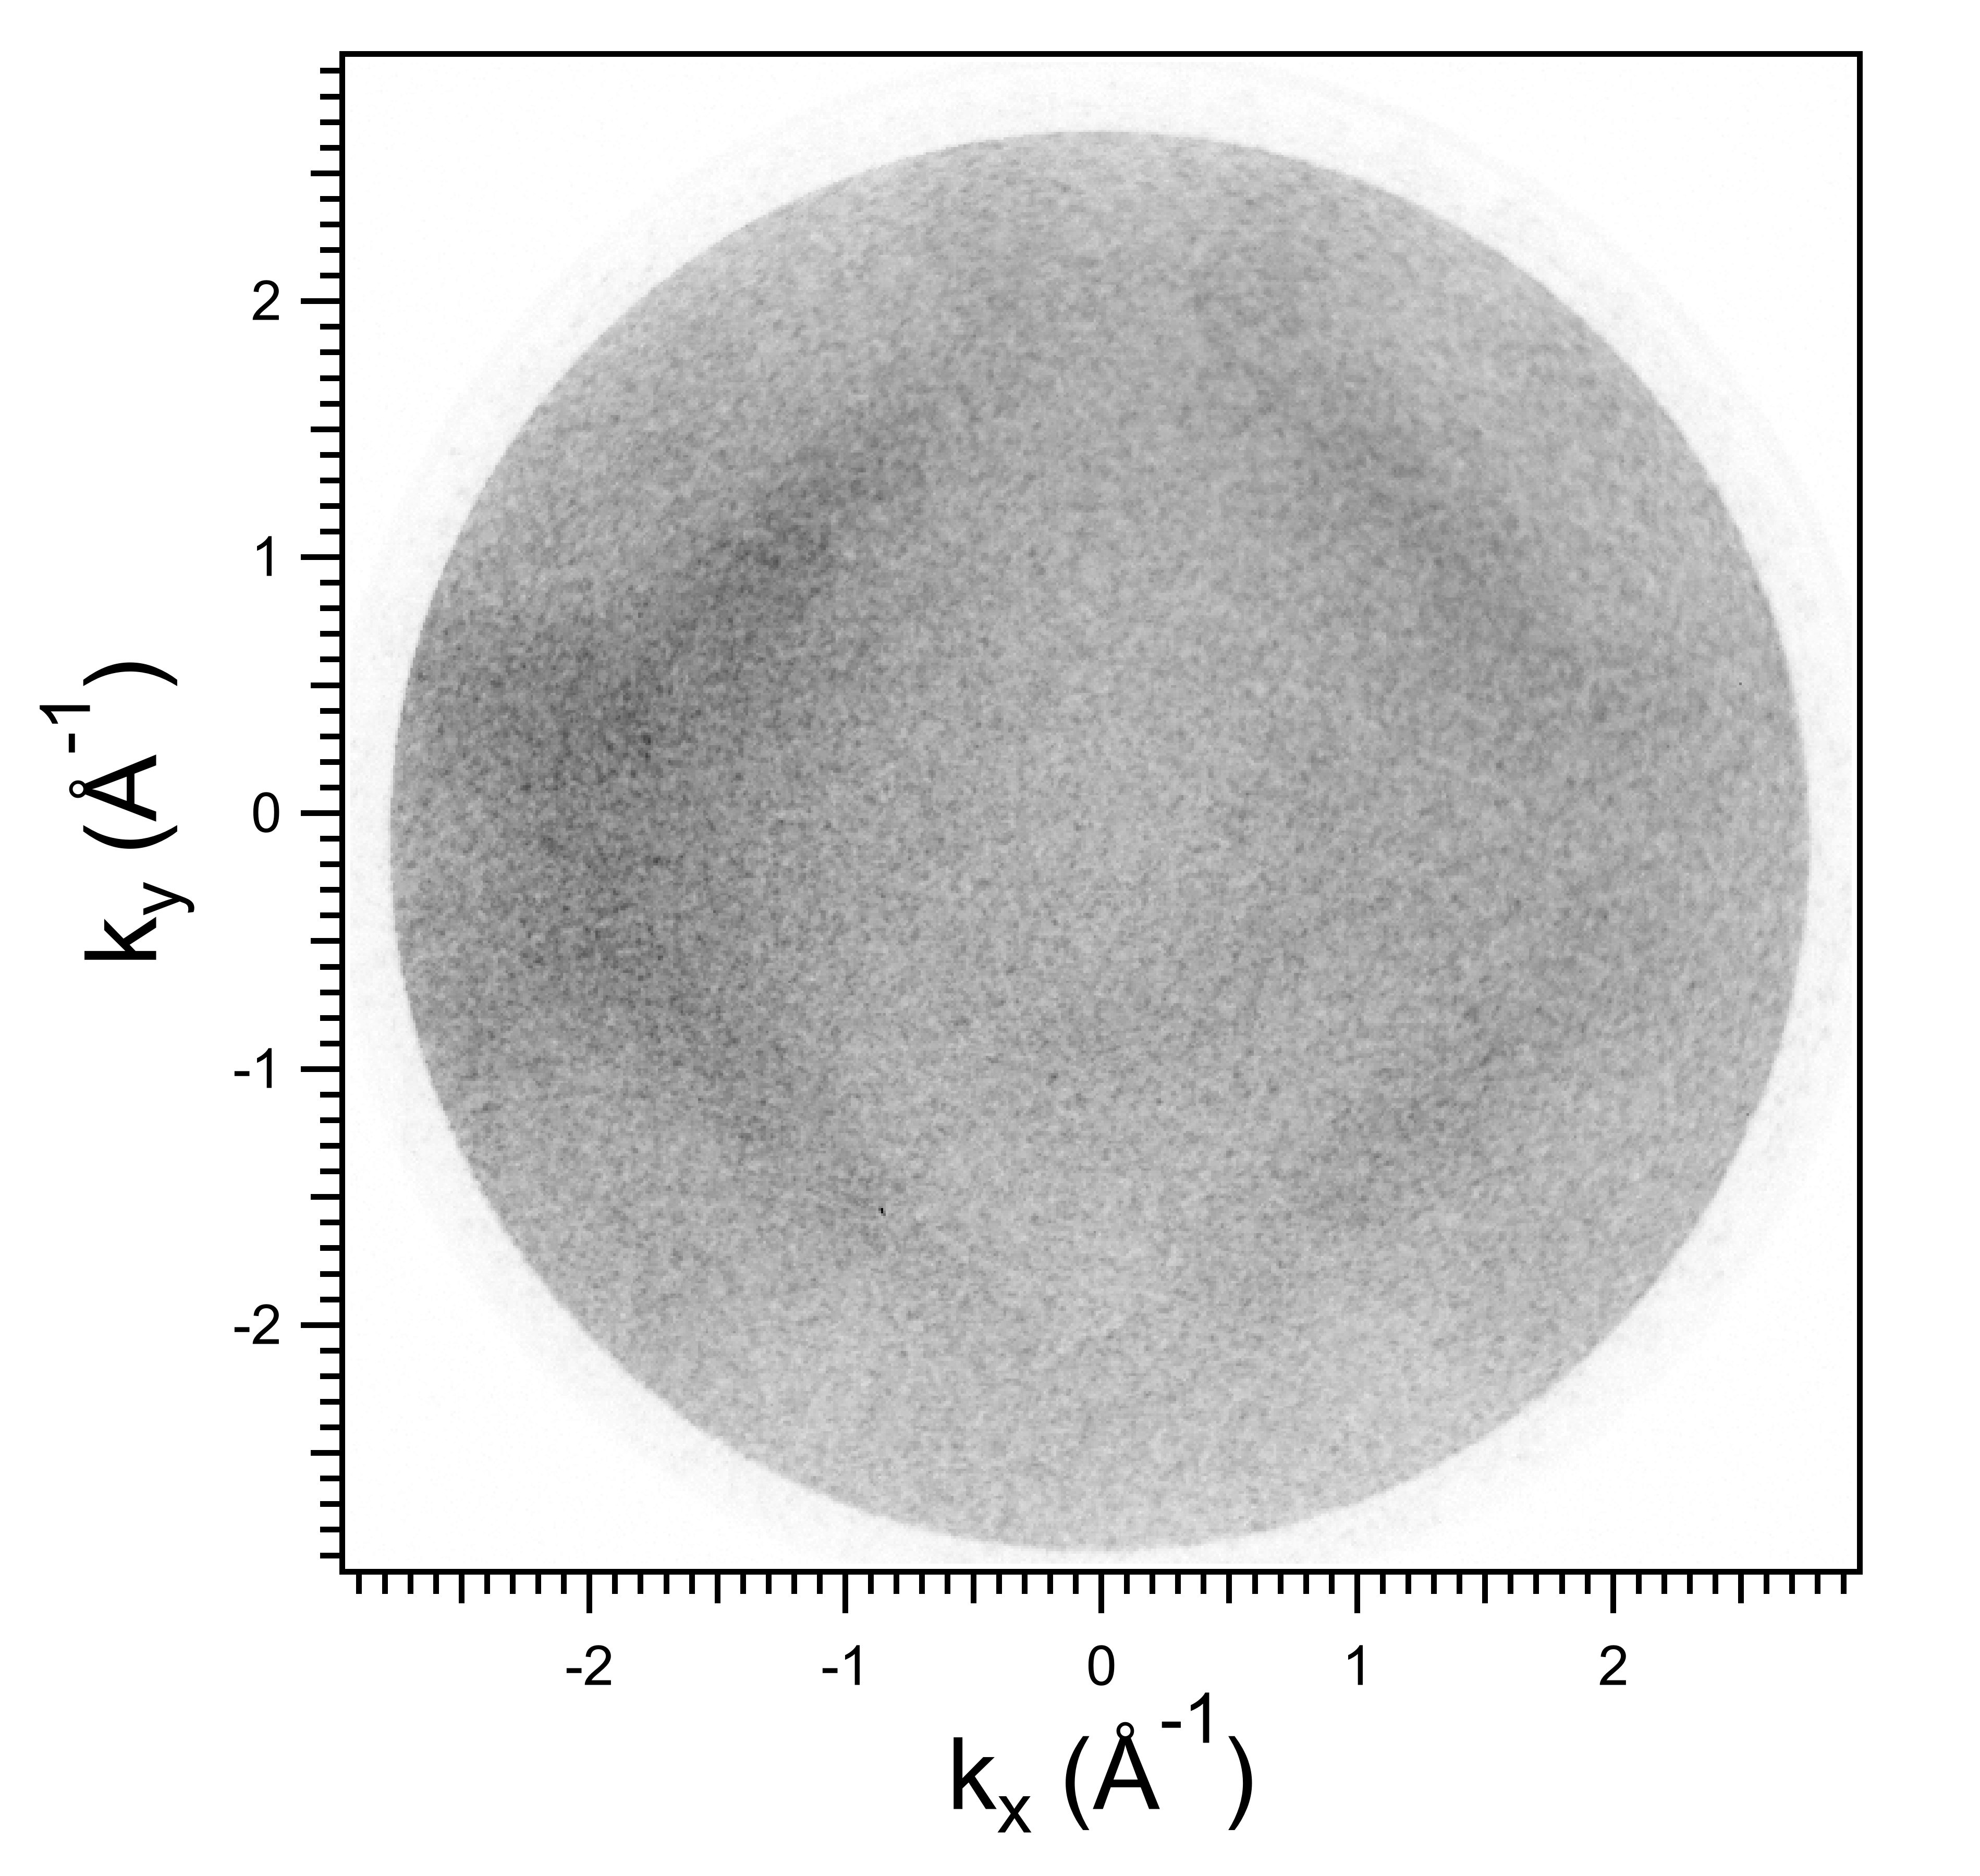
\includegraphics[height=5cm]{./content/pictures/FeO+5A/FeO_5A_34_80eV.png}
                \subcaption{Das Bild für eine kinetische Energie von \SI{34.80}{\electronvolt}, also \SI{0.70}{\electronvolt} Bindungsenergie.}
            \end{subfigure}
            \begin{subfigure}[t]{0.48\textwidth}
                \centering
                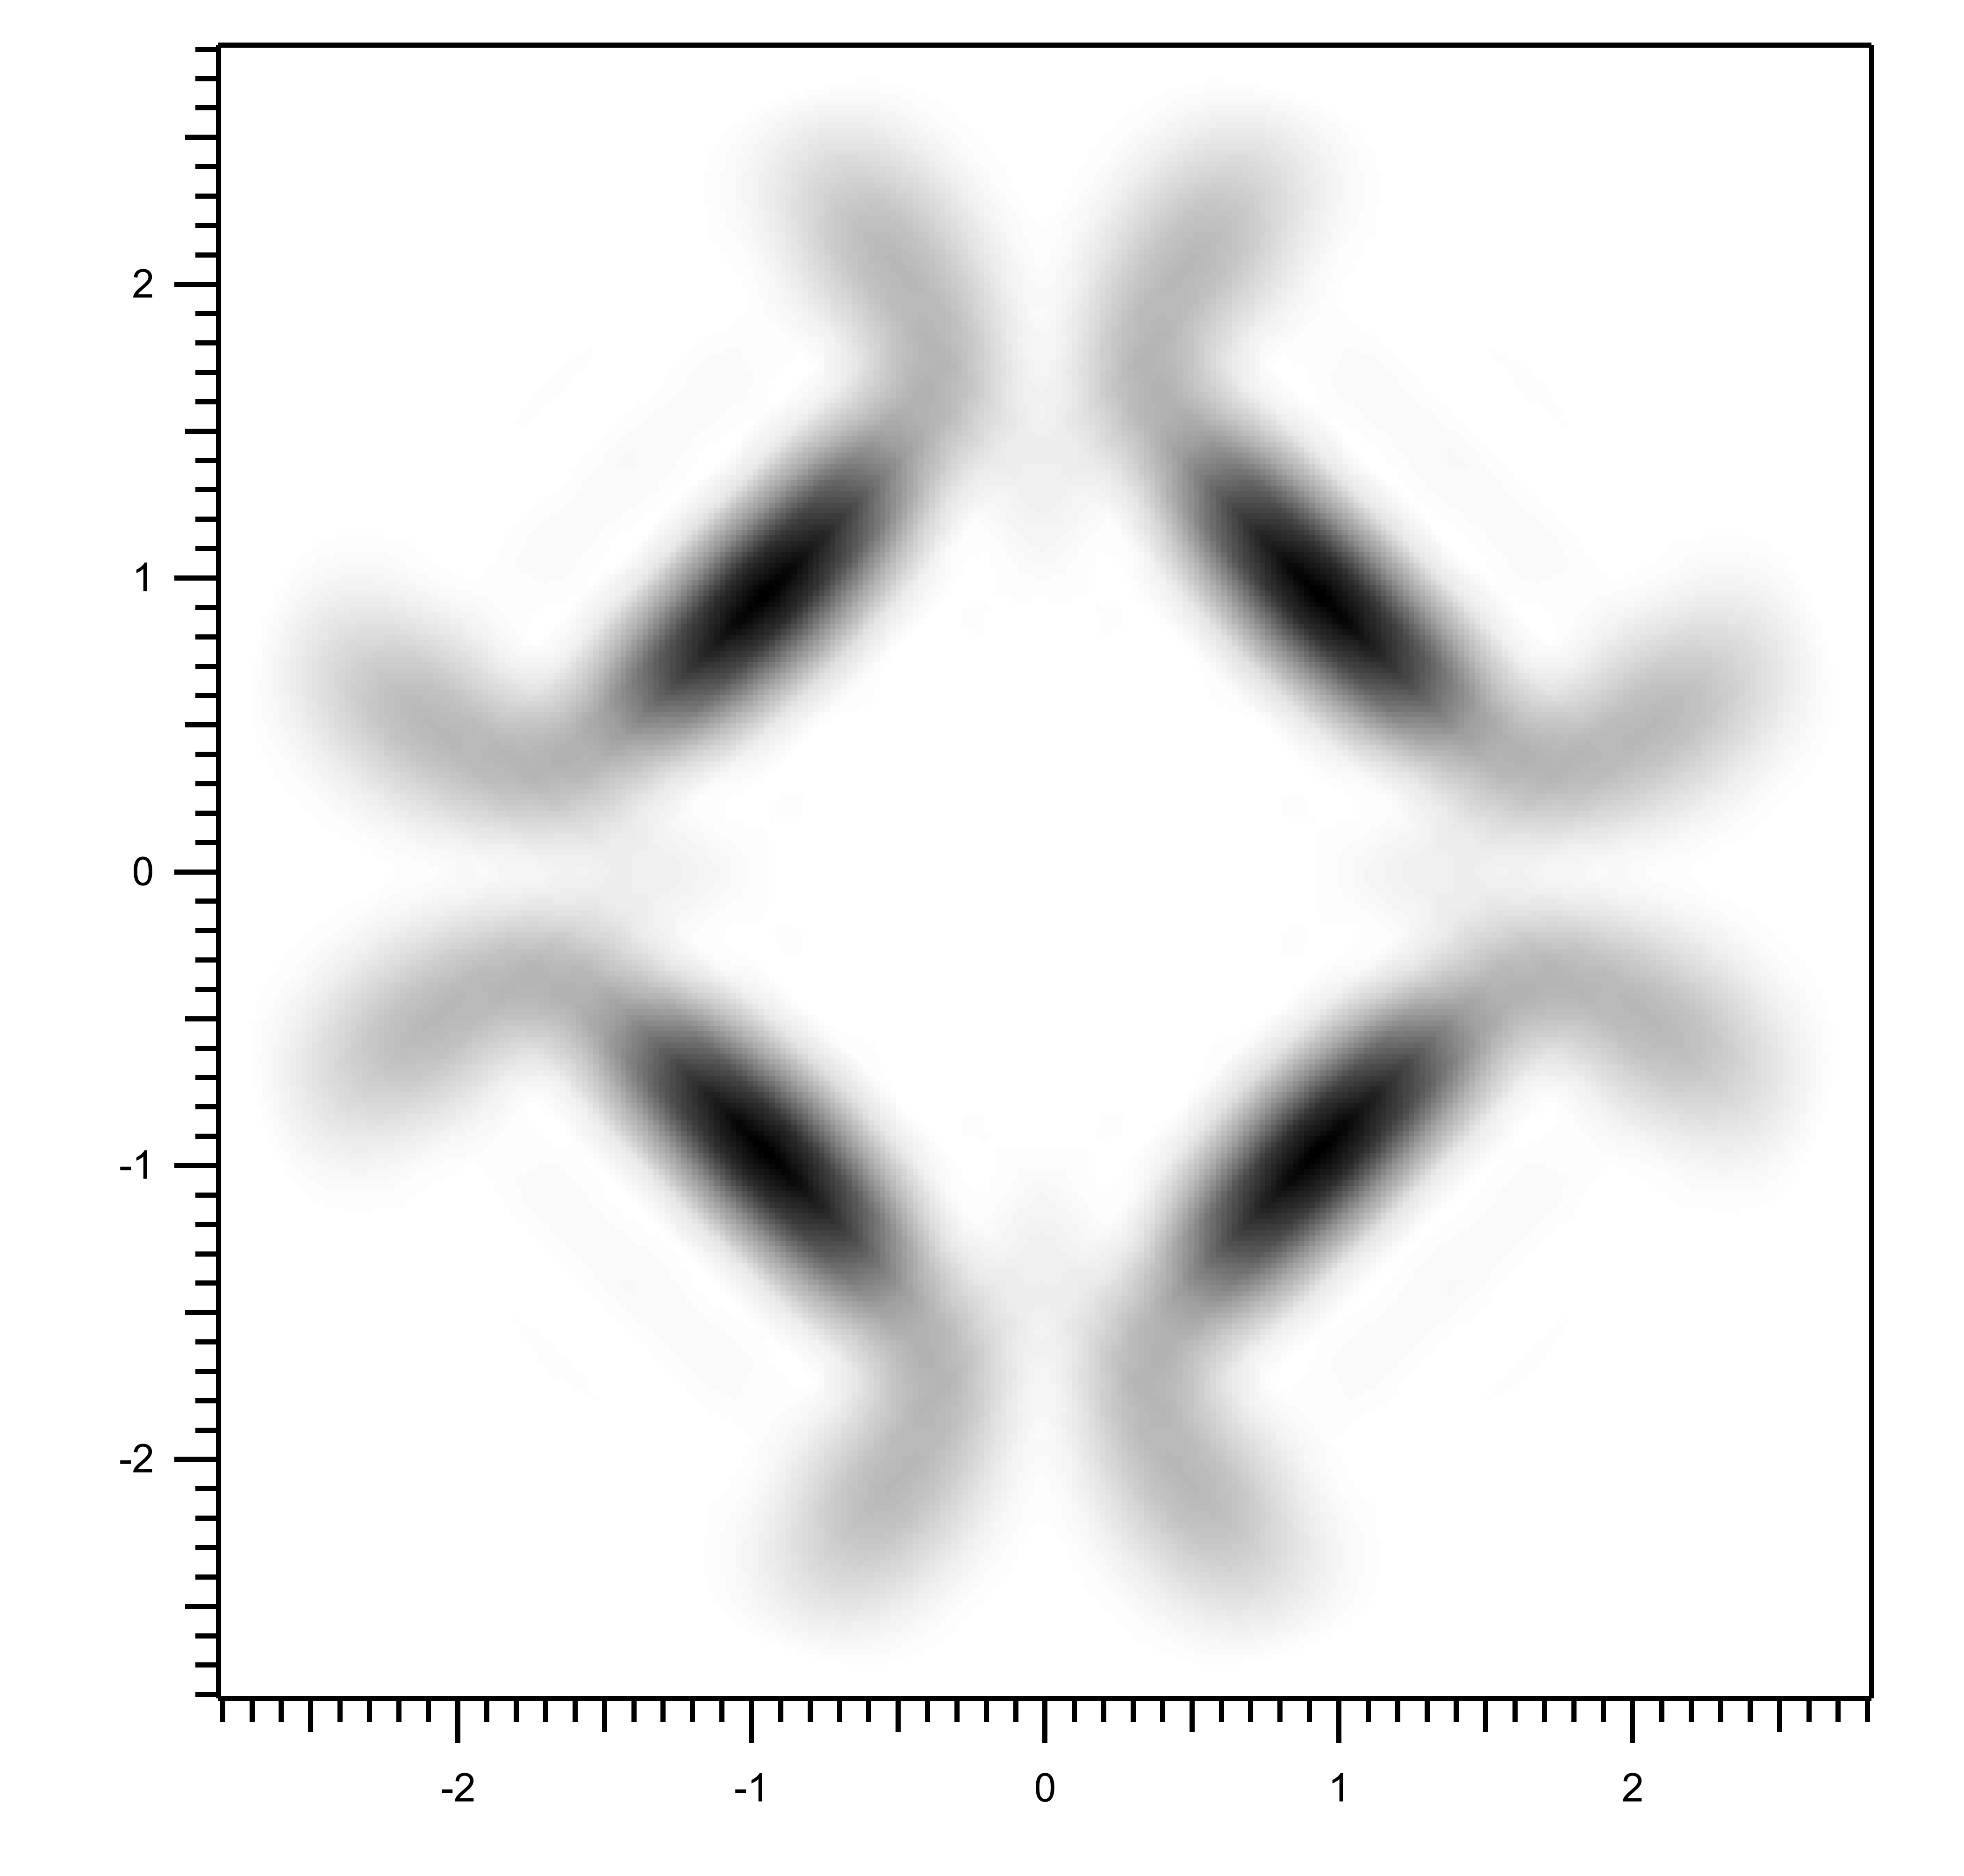
\includegraphics[height=5cm]{./content/pictures/FeO+5A/MO_LUMO_RT_RT.png}
                \subcaption{Das LUMO mit Symmetrisierung zweier um \SI{90}{\degree} verdrehten Übergitter.}
            \end{subfigure}
            \caption{Vergleich der gemessenen Intensitätsverteilung mit der des symmetrisierten LUMO.}
            \label{fig:FeO5A1}
        \end{figure}
        \begin{figure}
            \centering
            \begin{subfigure}[t]{0.48\textwidth}
                \centering
                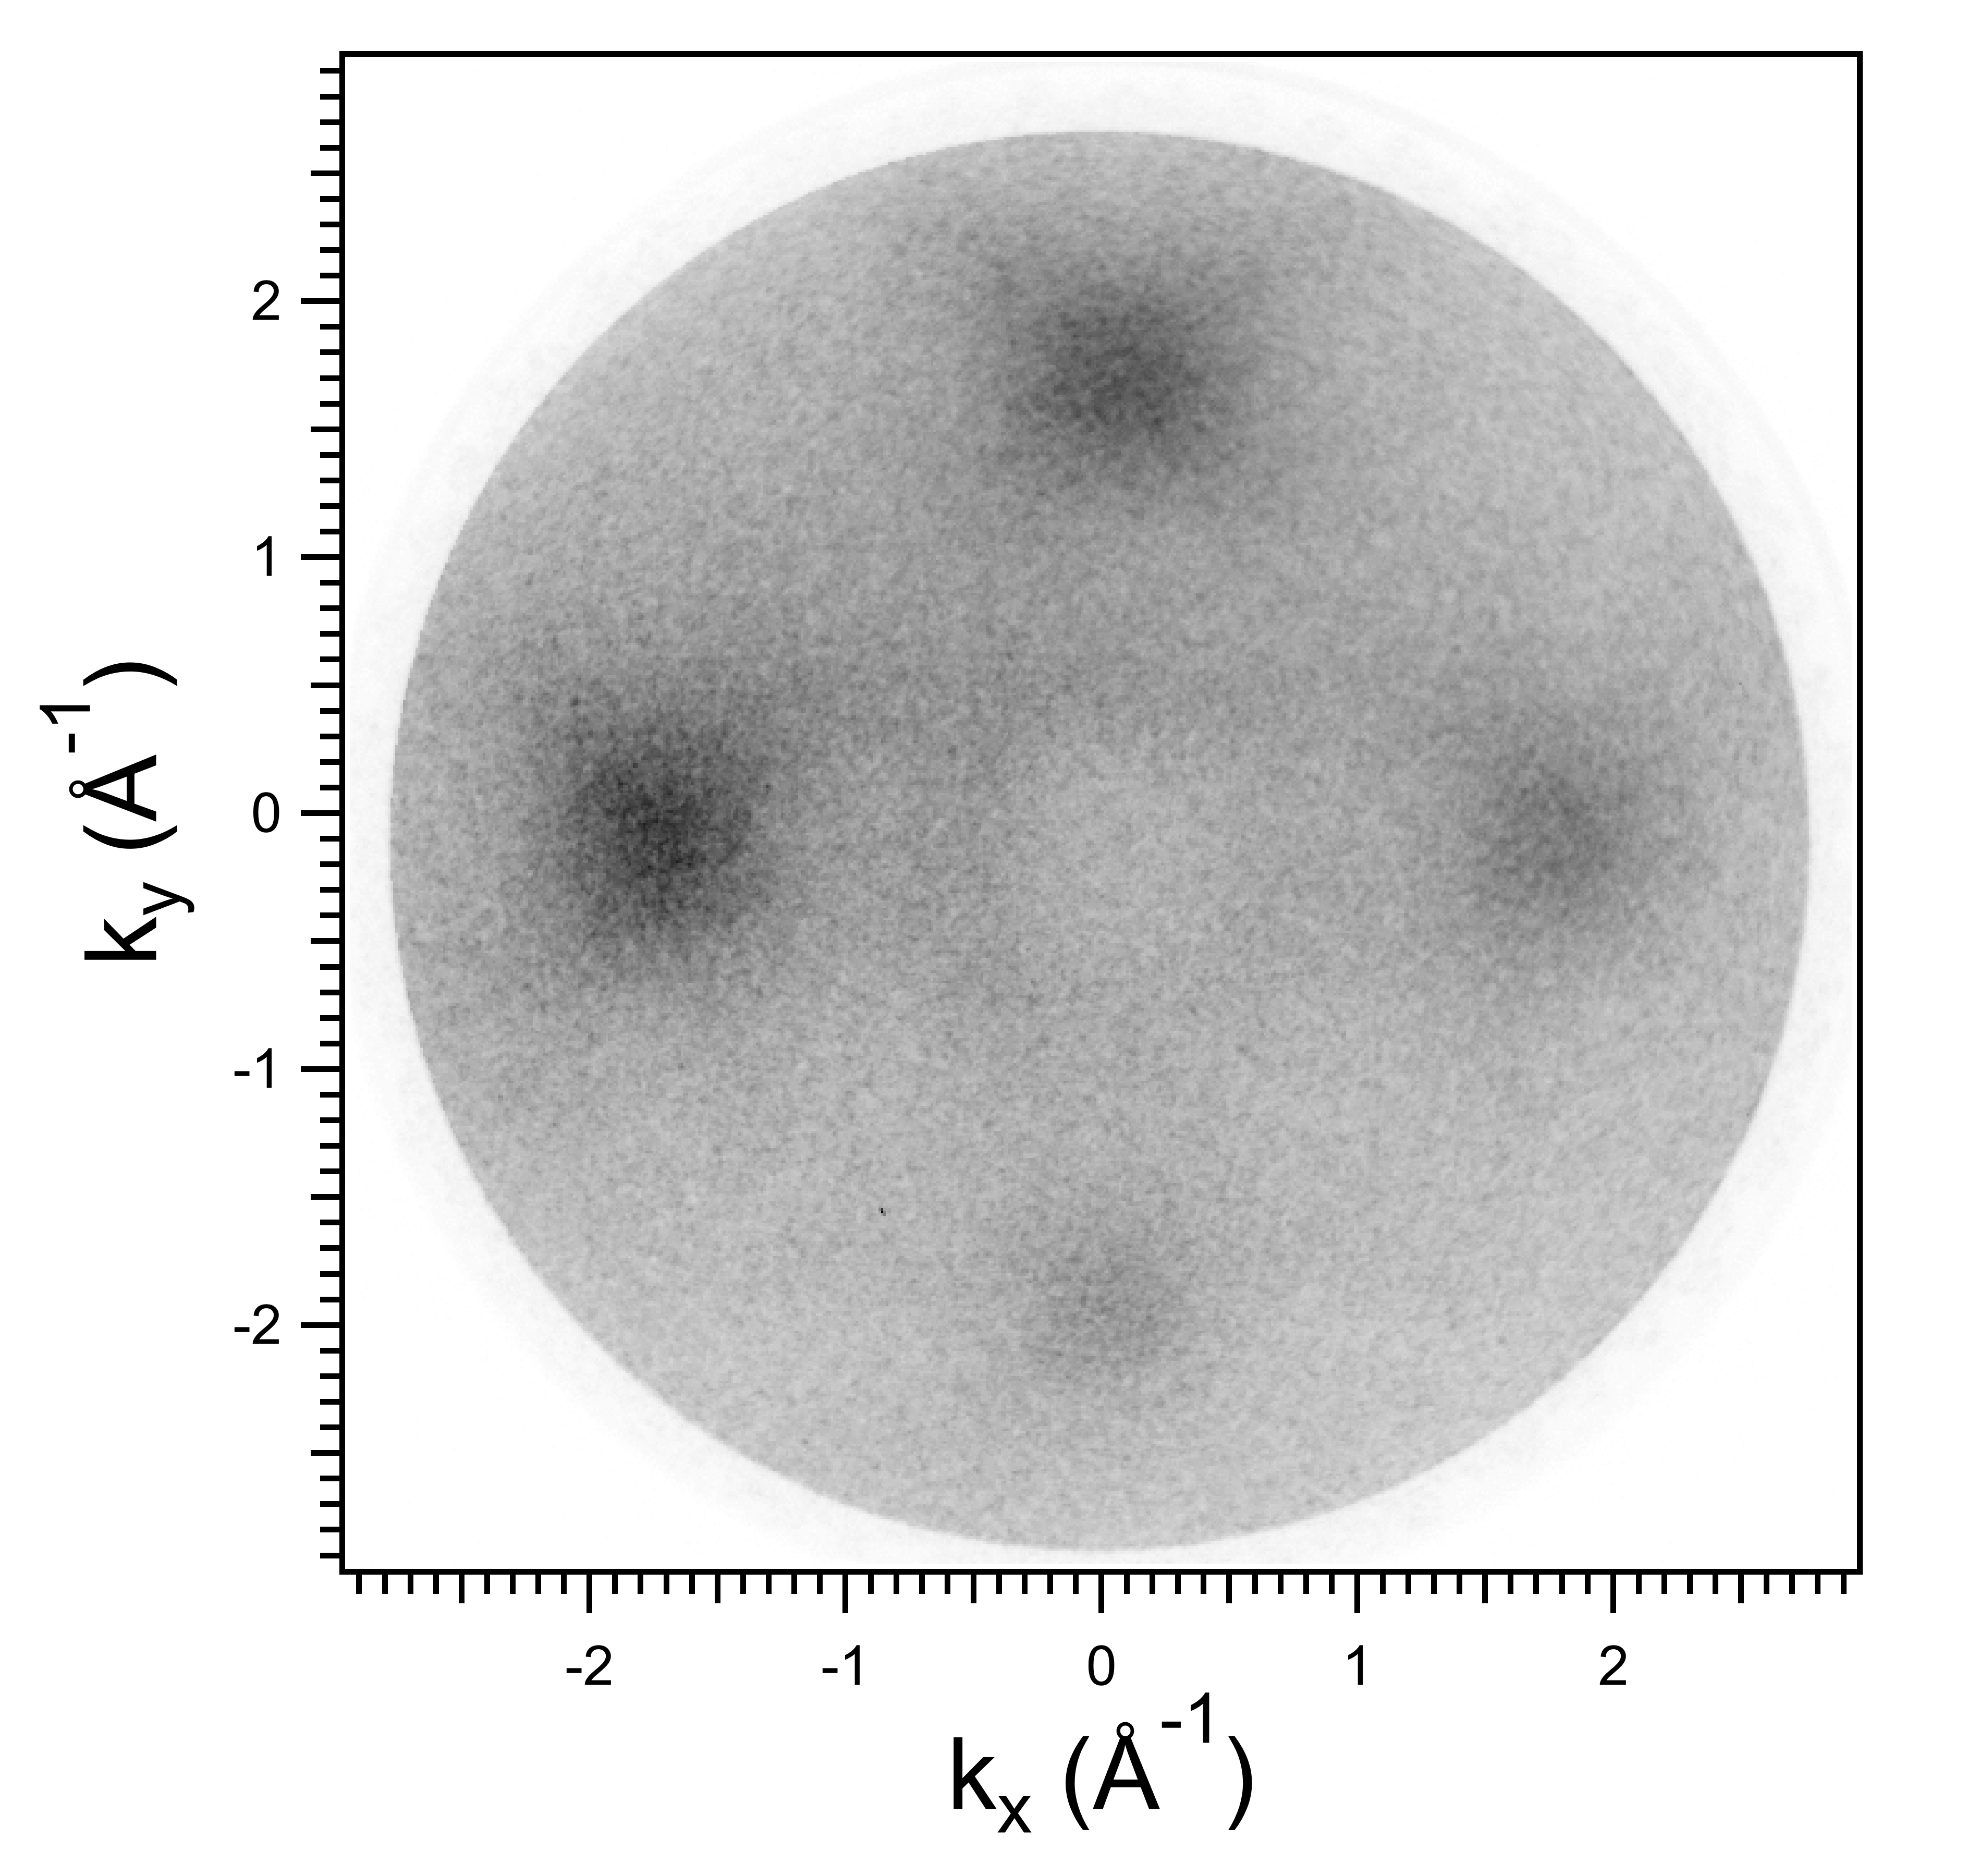
\includegraphics[height=5cm]{./content/pictures/FeO+5A/FeO_5A_33_75eV.png}
                \subcaption{Das Bild für eine kinetische Energie von \SI{33.75}{\electronvolt}, also \SI{1.75}{\electronvolt} Bindungsenergie.}
            \end{subfigure}
            \begin{subfigure}[t]{0.48\textwidth}
                \centering
                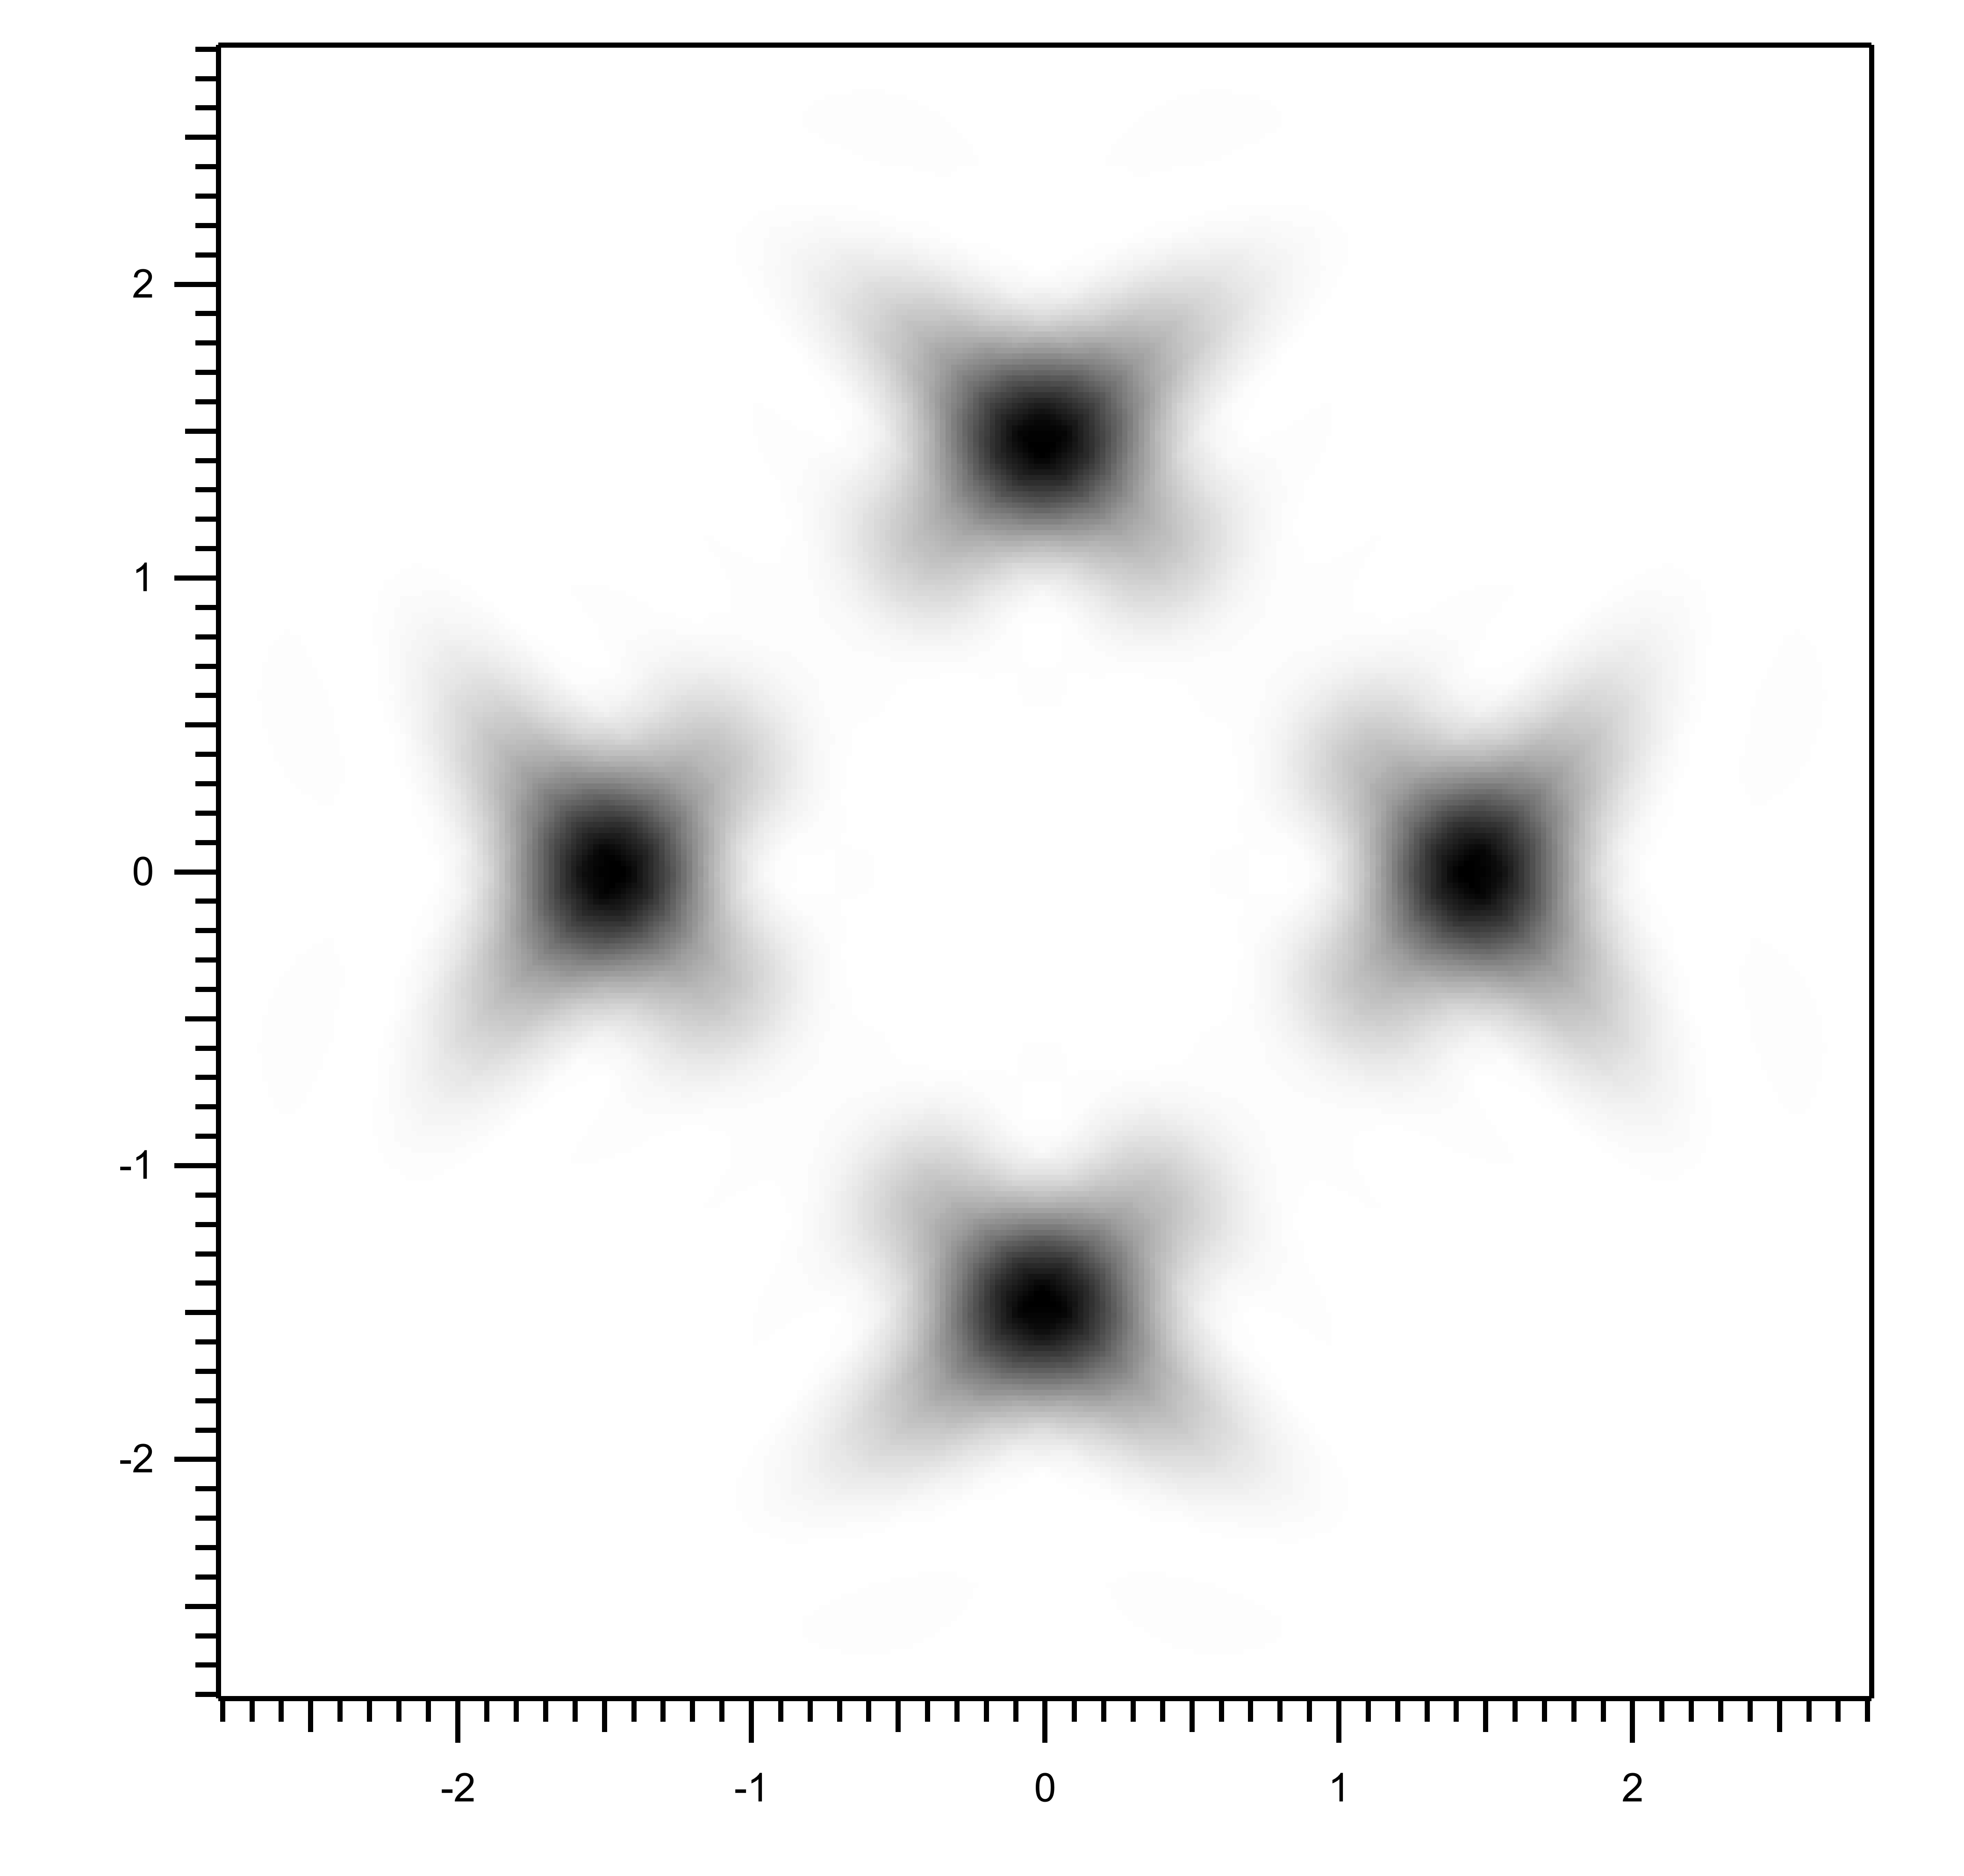
\includegraphics[height=5cm]{./content/pictures/FeO+5A/MO_HOMO_RT_RT.png}
                \subcaption{Das HOMO mit Symmetrisierung zweier um \SI{90}{\degree} verdrehten Übergitter.}
            \end{subfigure}
            \caption{Vergleich der gemessenen Intensitätsverteilung mit der des symmetrisierten HOMO.}
            \label{fig:FeO5A2}
        \end{figure}
        \begin{figure}
            \centering
            \begin{subfigure}[t]{0.48\textwidth}
                \centering
                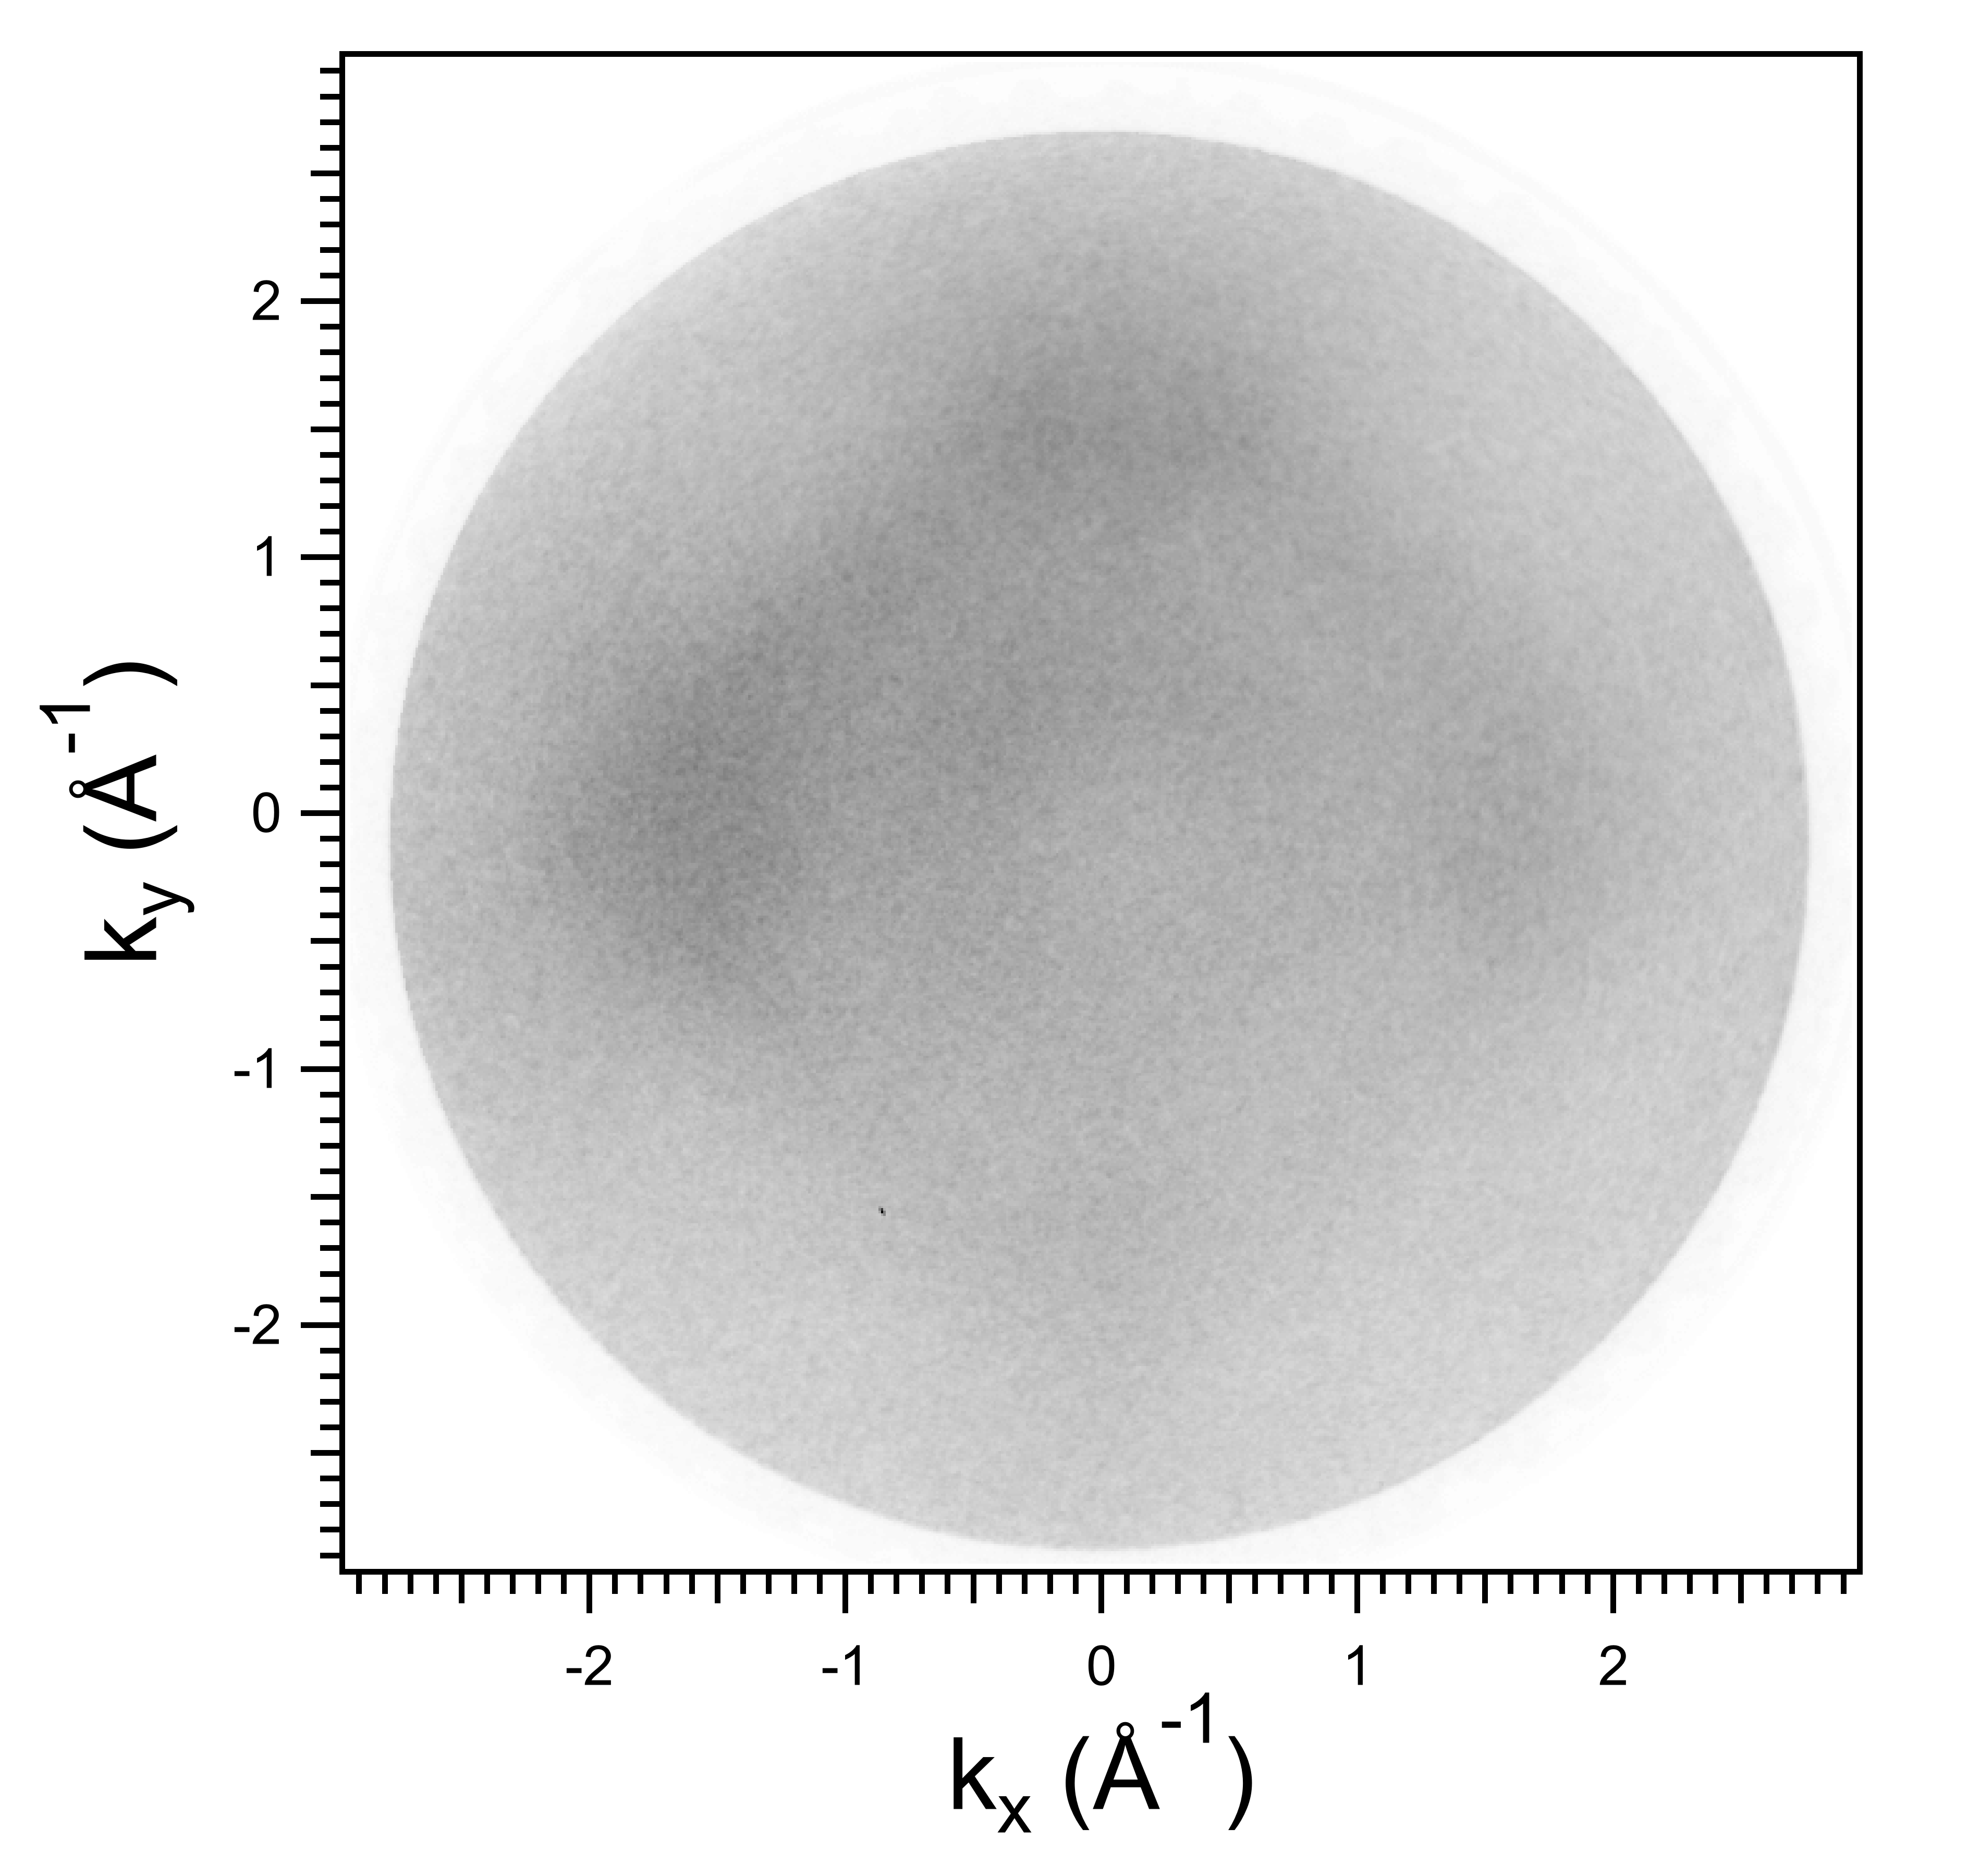
\includegraphics[height=5cm]{./content/pictures/FeO+5A/FeO_5A_32_15eV.png}
                \subcaption{Das Bild für eine kinetische Energie von \SI{32.15}{\electronvolt}, also \SI{3.35}{\electronvolt} Bindungsenergie.}
            \end{subfigure}
            \begin{subfigure}[t]{0.48\textwidth}
                \centering
                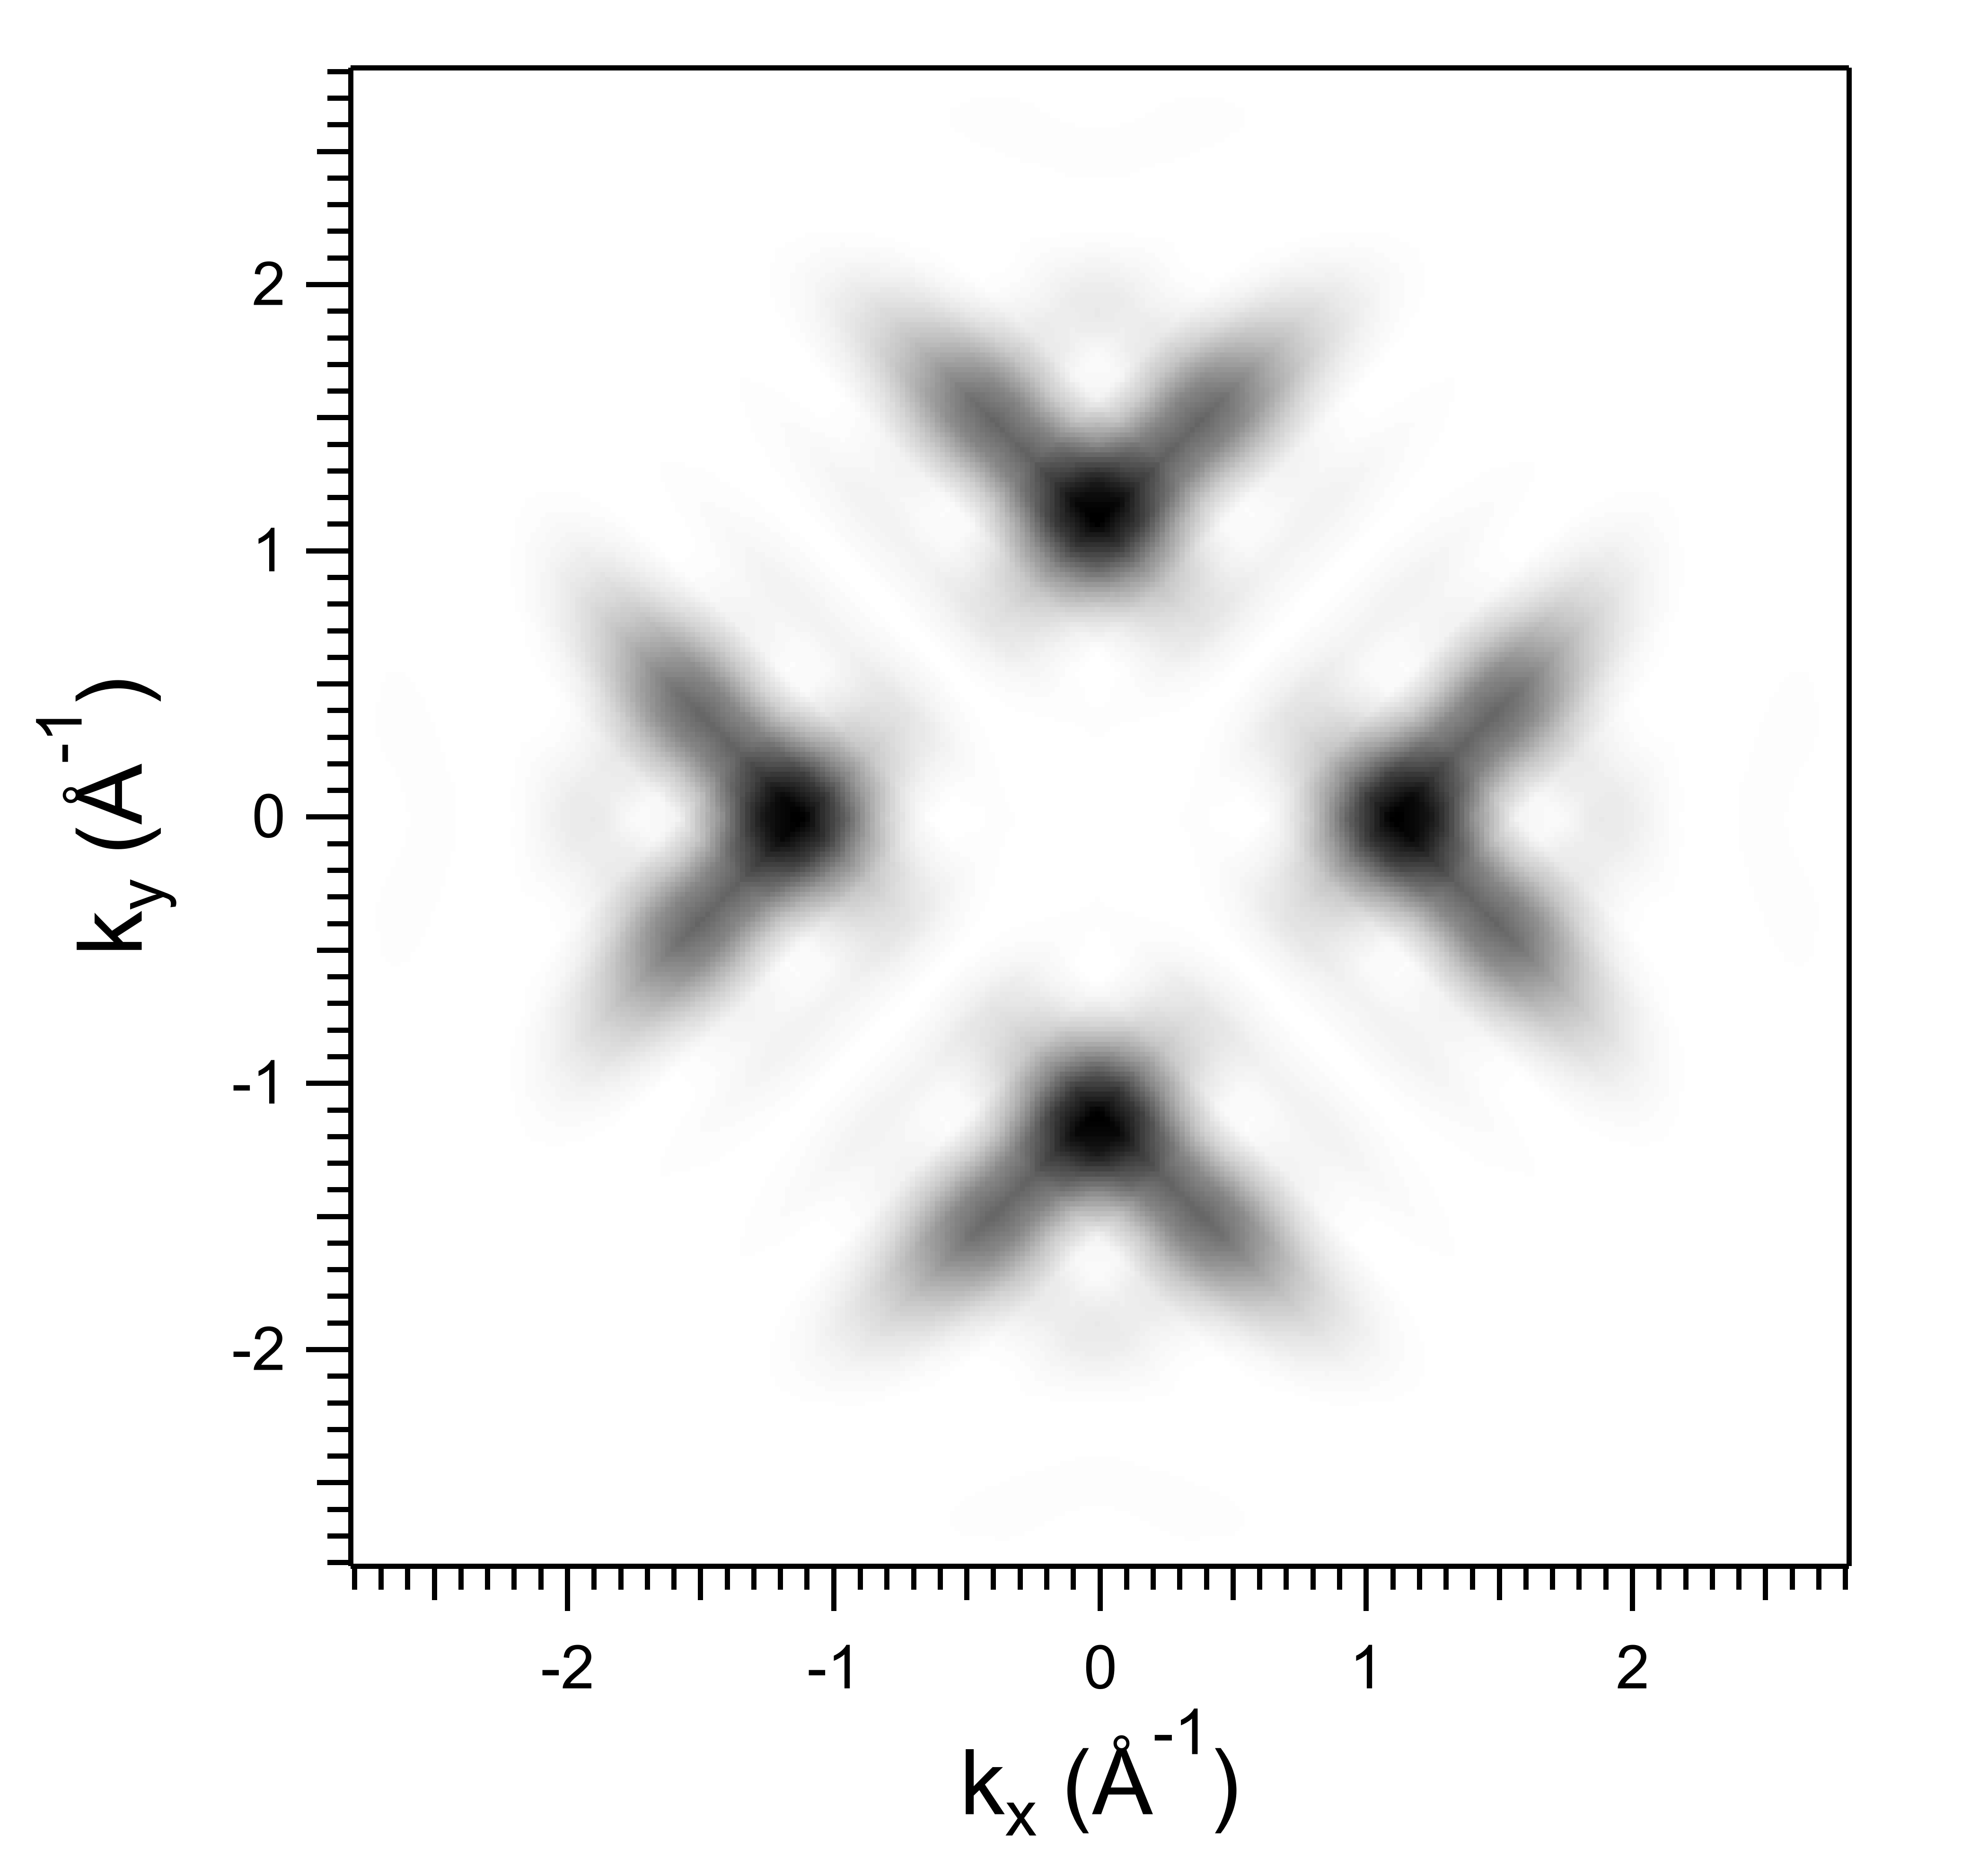
\includegraphics[height=5cm]{./content/pictures/FeO+5A/MO_HOMO1_RT_RT.png}
                \subcaption{Das HOMO-1 mit Symmetrisierung zweier um \SI{90}{\degree} verdrehten Übergitter.}
            \end{subfigure}
            \caption{Vergleich der gemessenen Intensitätsverteilung mit der des symmetrisierten HOMO-1.}
            \label{fig:FeO5A3}
        \end{figure}
        \begin{figure}
            \centering
            \begin{subfigure}[t]{0.48\textwidth}
                \centering
                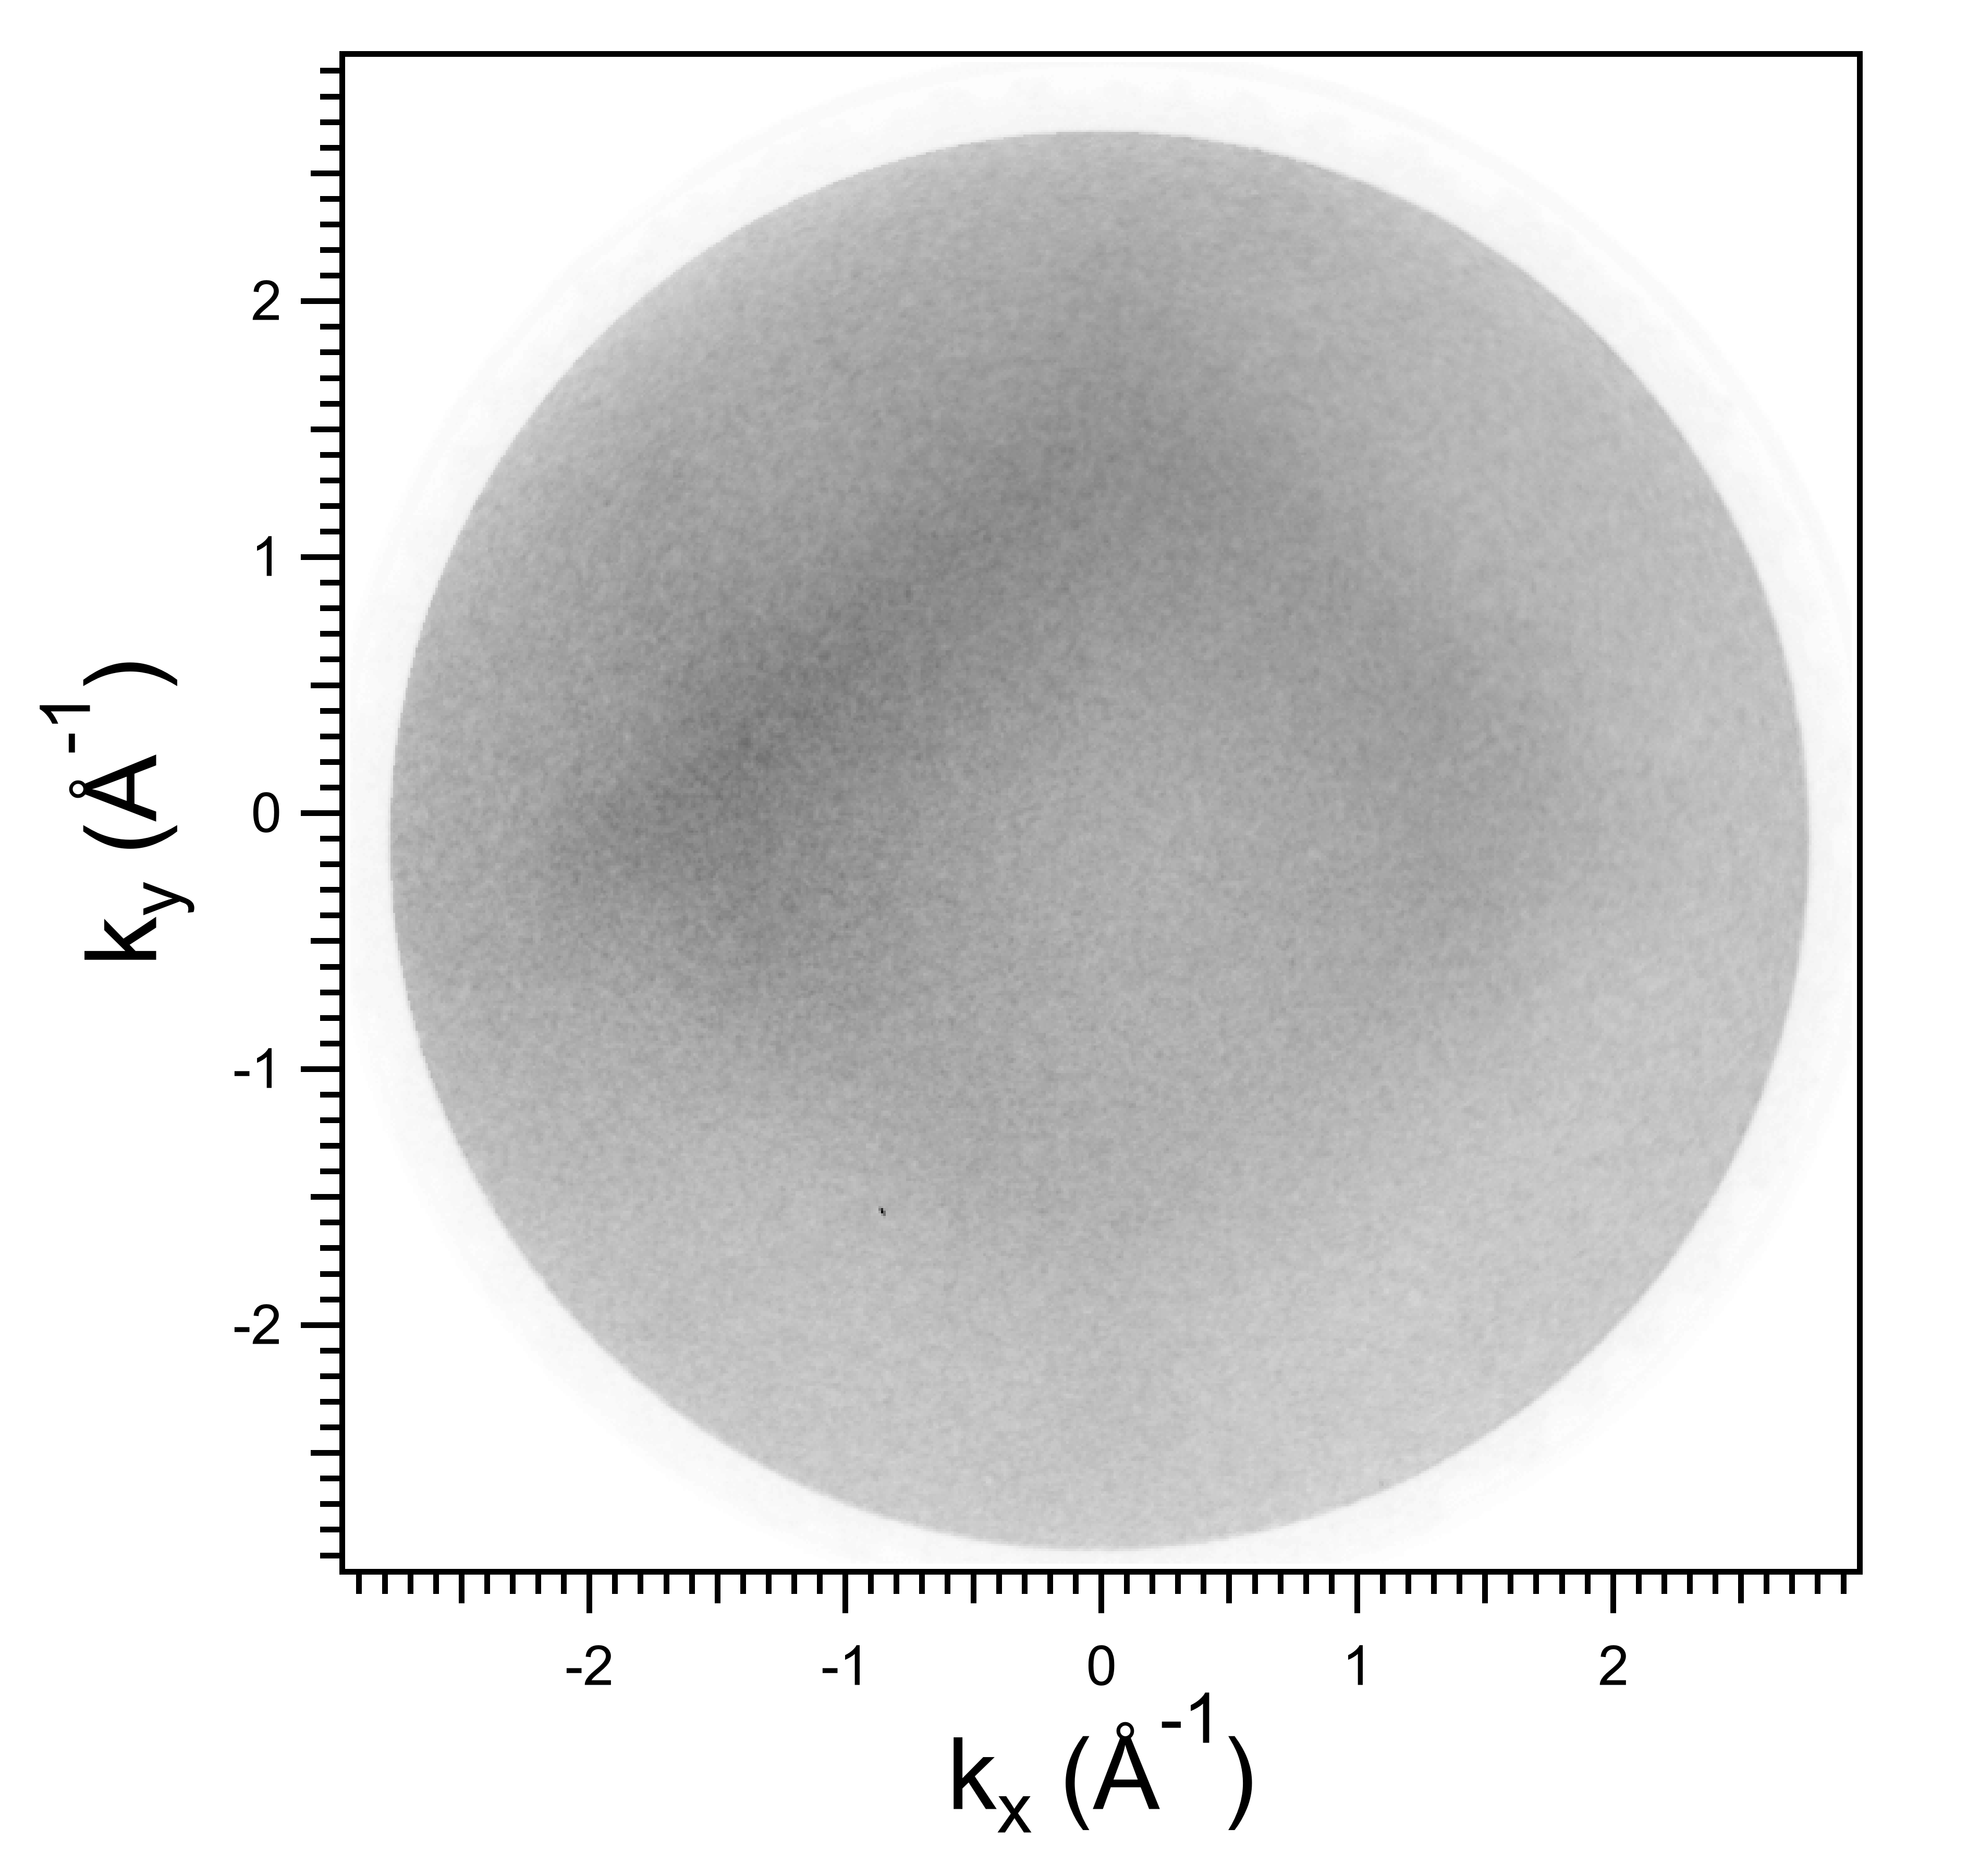
\includegraphics[height=5cm]{./content/pictures/FeO+5A/FeO_5A_30_95eV.png}
                \subcaption{Das Bild für eine kinetische Energie von \SI{30.95}{\electronvolt}, also \SI{4.55}{\electronvolt} Bindungsenergie.}
            \end{subfigure}
            \begin{subfigure}[t]{0.48\textwidth}
                \centering
                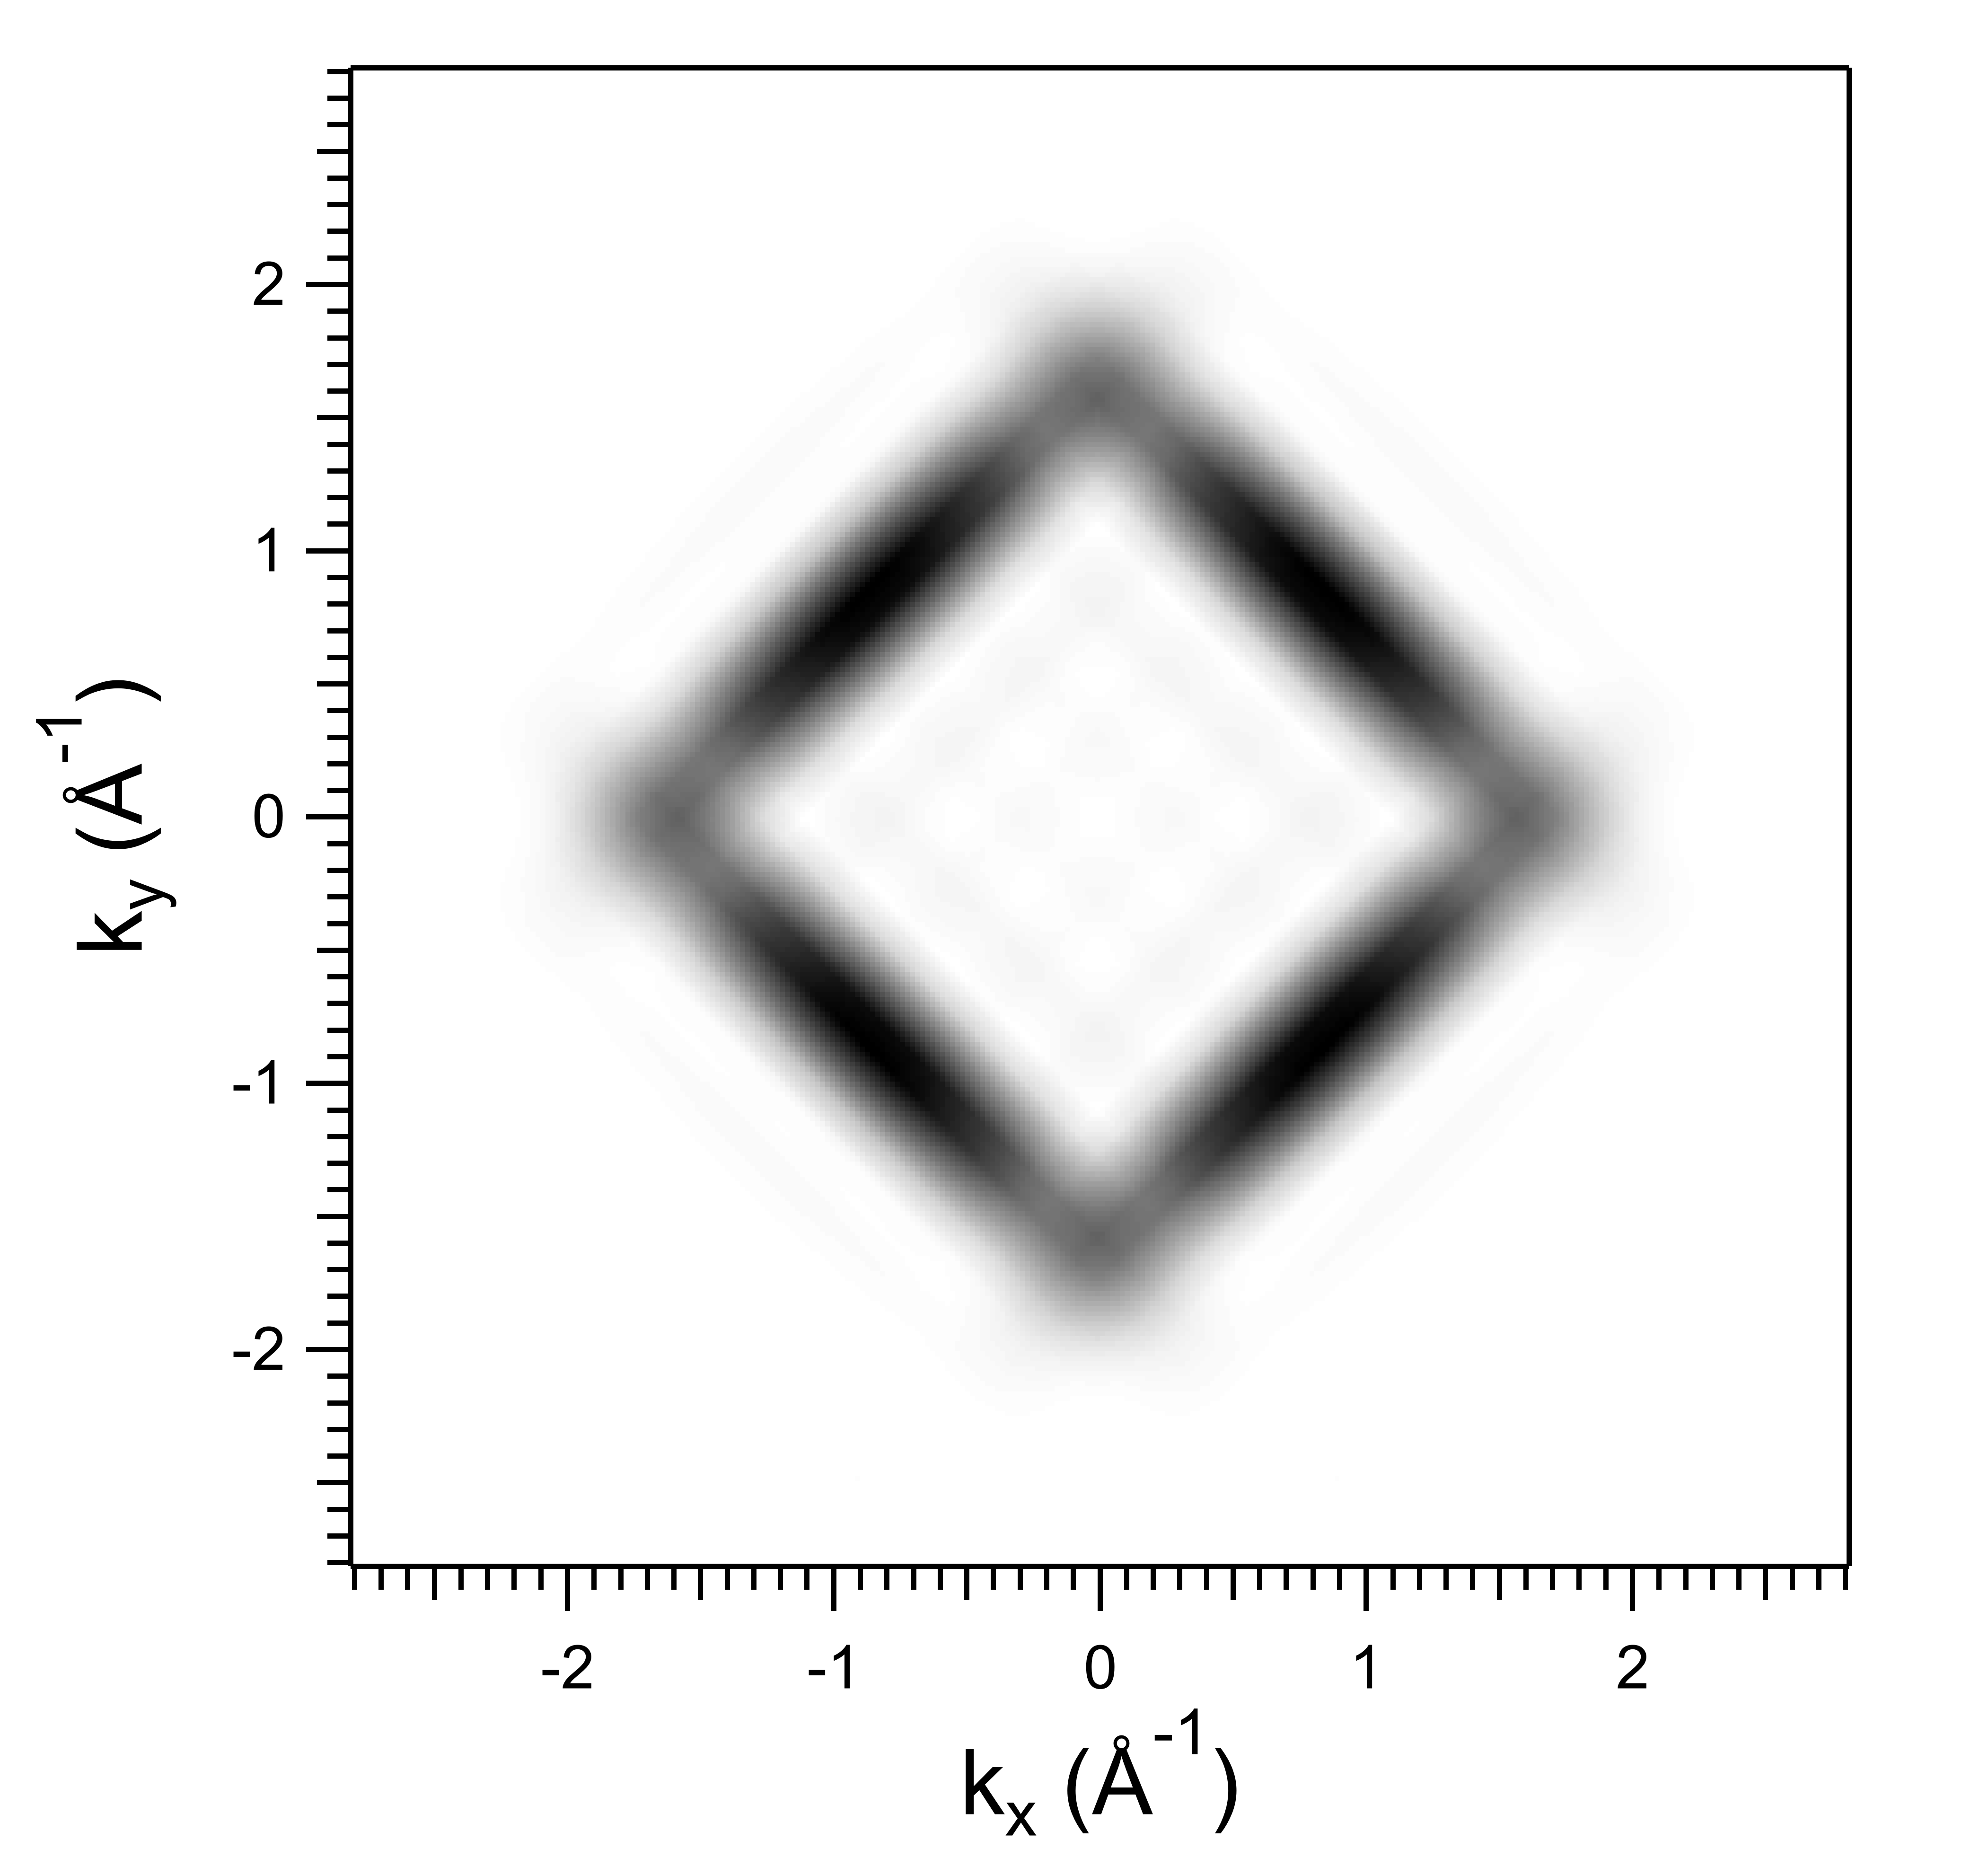
\includegraphics[height=5cm]{./content/pictures/FeO+5A/MO_HOMO2_RT_RT.png}
                \subcaption{Das HOMO-2 mit Symmetrisierung zweier um \SI{90}{\degree} verdrehten Übergitter.}
            \end{subfigure}
            \caption{Vergleich der gemessenen Intensitätsverteilung mit der des symmetrisierten HOMO-2.}
            \label{fig:FeO5A4}
        \end{figure}
        Das Aufdampfen wie einer Monolage Pentacene brachte erneut kein homogenes und von einer geordneten Struktur herrührendes LEED-Bild zustande.
        Im Widerspruch zu dem nicht Vorhandensein entsprechnder Beugungsreflexe und damit sich die Moleküle nicht auf der Oberfläche ordnen sind in den Tomographiebildern Merkmale von Molekülen zu erkennen.
        Diese Merkmale können sich nur ausbilden, wenn sich die Moleküle regelmäßig und in gleicher Orientierung anordnen.
        Anderenfalls würden sich die Photoemissionströme überlagern und es gäbe verschwommene Bilder.
        Einige Zuordnungen sind in den Abbildungen \ref{fig:FeO5A1} bis \ref{fig:FeO5A4} zu finden.
        \begin{figure}
            \centering
            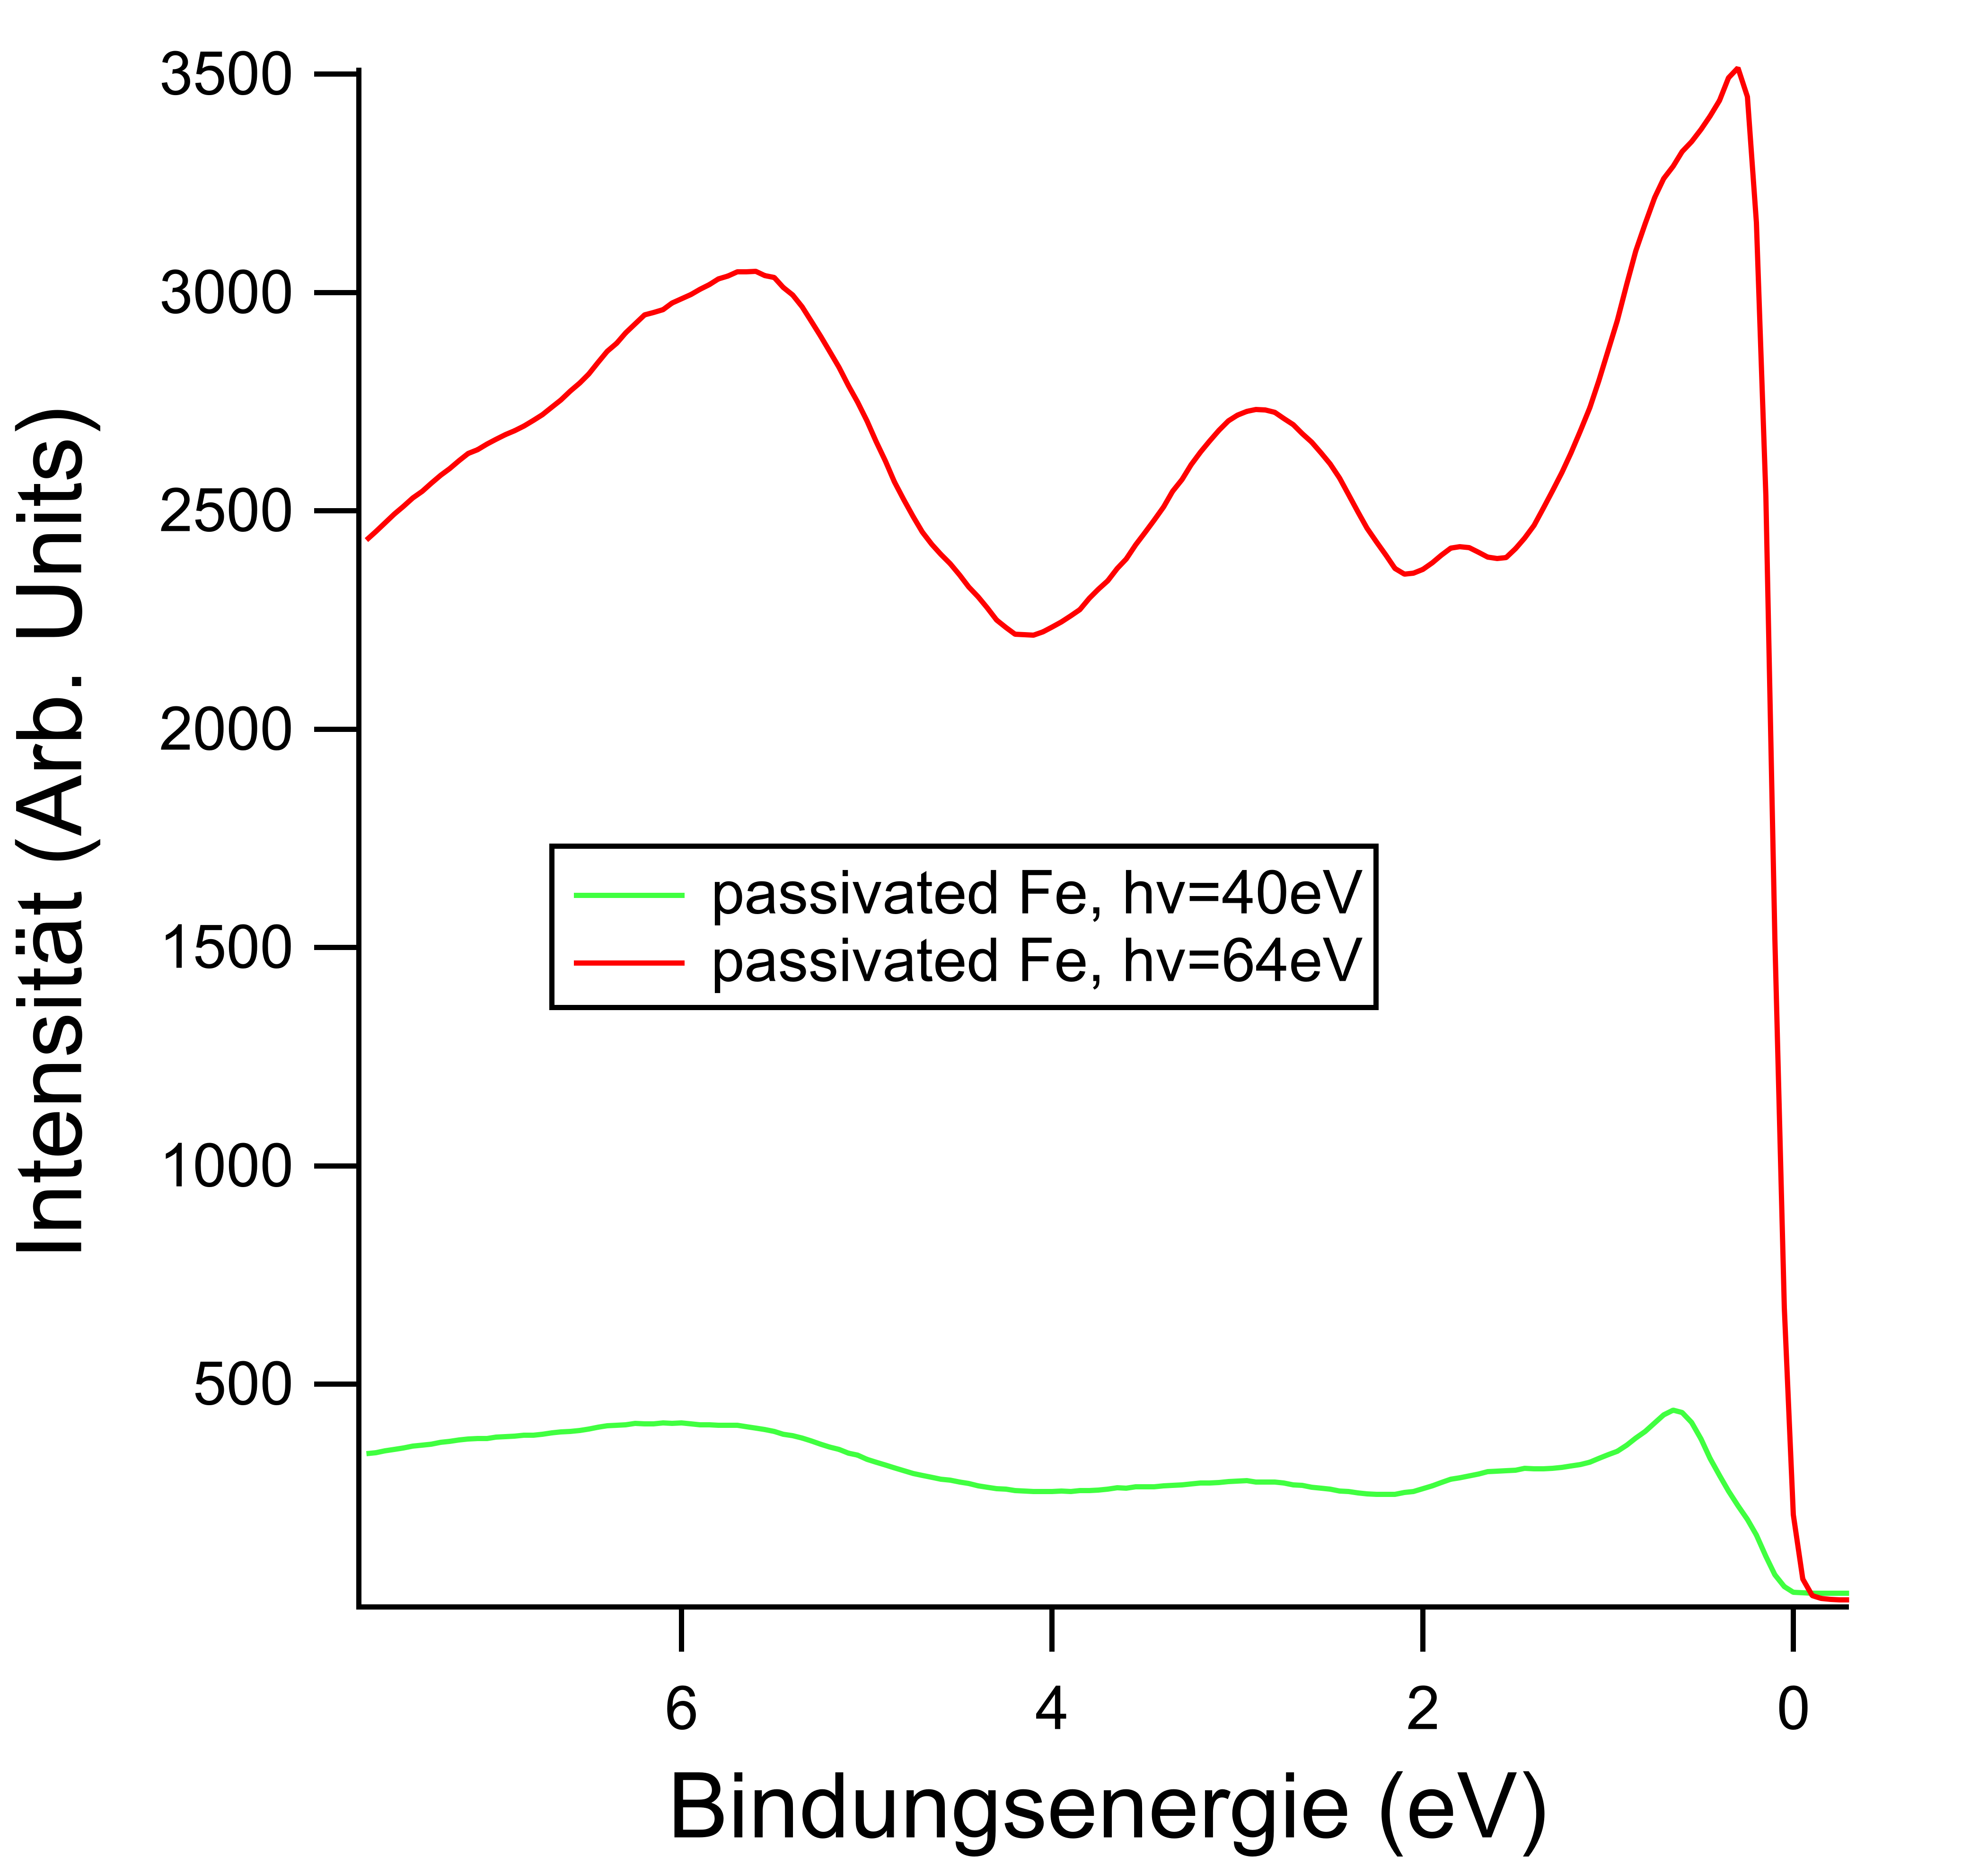
\includegraphics[height=5cm]{./content/pictures/pFe/Photonenenergie.png}
            \caption{Vergleich des VB-Spektrums bei \SI{64}{\electronvolt} und \SI{40}{\electronvolt} Photonenenergie des passivierten Eisens.}
            \label{fig:Photonenenergie}
        \end{figure}
        Allerdings ist die eindeutige Zuordnung recht schwierig, da eine Referenzmessung des Substartes bei entsprechnder Photonenenergie nicht aufgenommen wurde.
        Bei einer anderen Photonenenergie aufgenommene Spektren lassen sich nur schwer als Vergleich heranziehen, da diese deutliche Unterschiede aufweisen können.
        Als Bespiel sind hier in \autoref{fig:Photonenenergie} zwei Spektren des passivierten Eisens dargestellt bei unterschiedlicher Photonenenergie.
        Klar zu erkennen ist schon der Unterschied in der Gesamtintensität, was durch den unterschiedlichen Photonenfluss der Beamline für verschiedene Energien zustande kommt.
        Aber auch bei der betrachtung der winkelaufgelösten Bilder sind klare Unterschiede hinsichtlich der Merkmale erkennbar.
        Teilweise zeigen die Bilder bei den gleichen Energien wie die HOMO bis HOMO-2 Orbitale sehr ähnliche Signale wie mit den Molekülen.

        Es kann davon ausgegangen werden, dass es sich bei der Wechselwirkung um die Chemisorption handelt, denn auch das LUMO wird besetzt.
        Um dies zu erlangen muss vorher Ladung zwischen dem Molekühlen und dem Substart ausgetauscht worden sein, was das Merkmal der Chemisorption ist.

  
    \section{NOTIZEN}
    \subsection{datendeutung}
        \begin{itemize}
            \item Zuordnung des Fe3p Peaks schwer. Manche sagen sechs Peaks voraus \cite{FeO_14, FeO_17, FeO_15} wegen der Finestruktur, andere zwei (Fe2+, Fe3+) \cite{FeO_15, FeO_11, FeO_10, FeO_7} manche drei (Fe2+, Fe3+tetra, Fe3+octa) \cite{FeO_12}. es kommt dabei auf das Material an, zum Identifizieren ist es also schwierig durch den einen Peak.
            \item Die Bindungsnergie des $\ce{Fe}^{2+}$ liegt bei \SI{53.7}{\electronvolt} und die des $\ce{Fe}^{3+}$ bei \SI{55.6}{\electronvolt} \cite{FeO_7}.
            \item Der Peak des reinen Eisens (\autoref{fig:XPSFe3p_FeO}) ist nicht dem Fe2+ oder Fe3+ zuzuornden. FeO besitzt hingegen nur Fe2+, ist aber recht anfällig weiter zu oxidieren, so dass sich ein Fe3O4 (Fe2+, Fe3+tetra, Fe3+octa) oder Fe2O3 (nur Fe3+) Film bilden kann. 
            \item Bei dem O1s Peak ist man sich einig, dass sich der Hauptpeak nicht verschiebt, eine Unterscheidung der verschiednen Eisenoxide ist also damit nicht möhlich. es können zusätzlich Peaks durch Adsorbate (z.B. OH) auftauchen.
            \item Der  $\ce{O}_{1\text{s}}$ O2- Peak liegt bei \SI{529.7}{\electronvolt} \cite{FeO_9} OH- bei \SI{531.2}{\electronvolt} \cite{FeO_9}., \SI{530.1}{\electronvolt} \cite{FeO_15} (unabhängig welches Eisenoxid).
            \item XAS-Messungen mit Teilelektronen ausbeute von Sekundärelektronen bei einer Energie von $E_\text{Kin} = \SI{7}{\electronvolt}$.
            \item XAS Messungen wurden duch Multiplikation an Preedge ausgerichtet, dann wurde ein linear Untergrund abgezogen (pre-edge gefittet) und anschließend die Preedge auf Null gesetzt und die Postedge auf 1 (durch Division)
            \item Das XMCD Signal sollte für L3 und L2 umegkehrt sein, wenn es Ferromagnetisch ist, Signal lässt sich aber nur bei L3 erkennen.
            \item Auch XMLD für Antiferromagnetismus auf Grund der nicht spärischen Oribtale durch die Spin-Bahn-Kopplung (Spins ausgerichtet) \cite{stohr_magnetism_2006} - kann auch eben sein, dass die Spins nicht ausgerichtet waren. T war unter Neel Temperatur.
            \item Fermikante beim Isolator wie \ce{FeO} (was vermutet wird vorliegen zu haben) ist schwierig (Austrittsarbeit des Analyseres liegt bei \SI{5.07}{\electronvolt}). Also bei reinem Eisen gefittet (ebenfalls schwierig da mit Peak des VB überlappt) und damit über die Austrittsarbeit des Analysators \SI{4.5}{\electronvolt} und der Photonenenergie die Bindungsenergie bestimmt.
            \item FeO kann durch ioneninduzierte Zerstäubung aus anderen Eisenoxiden gewonnen werden, da der Wirkungsquerschnitt für Sauerstoff dabei größer ist und somit diese in der Konzentration reduziert werden. \cite{FeO_12}
                  Dann verschwinden auch Signale des Fe3+ \cite{FeO_15}, Einen Einfluss auf das FeO hat das Sputtern wohl nicht \cite{FeO_12, FeO_15}.
            \item Abschnitt des Spektrums des FeO bei \SI{-1.02}{\electronvolt}, Beginn bei \SI{58.93}{\electronvolt} -> Austrittsarbeit des \ce{FeO} \SI{4.05}{\electronvolt}, da $h\nu = \SI{64}{\electronvolt}$
        \end{itemize}
        % Der $\ce{Fe}_{3\text{p}} (\SI{54.52}{\electronvolt})$ wie auch der $\ce{O}_{1\text{s}} (\SI{529.15}{\electronvolt})$ lassen sich durch einen Peak fitten.

    \subsection{Ideen}
    \begin{itemize}
        \item Bandstruktur von FeO, Fe3O4, etc.
        \item Bandstruktur NiO? Spin?
        \item Bandstruktur mit Molekülen - Oberflächenzustände? Extra Features
        \item Austrittsarbeiten
    \end{itemize}

    \subsection{Anmerkungen}
    \begin{itemize}
        \item Voigt ist eine Faltung aus Lorentz, der natürlichen Linienbreite, ihre Inverse ist proportinal zur Lebenszeit des Zustands. Gauß hingegen nimmt die experimentelle Verbreiterung auf.
        \item Die Fermikante wird aus einer Faltung aus Gauß und ??? gefittet. Gauß ist ebenfalls wieder für die experimentelle Verbreiterung zuständig. Die Stufenfuktion bildet die Verbreiuterung durch die Temperatur und auch die Besetzung wieder.
        \item 
    \end{itemize}

    \subsection{Überbleibsel/ToDos}
    \begin{itemize}
        \item Sieht Features später Zuordnung
        \item Ändert sich was
        \item Verbreiterung Lebenszeit, Linienbreite Photonenquelle, Thermisch, Analysator
        \item peaks in integrierten Spektren zugeordnen
    \end{itemize}

    % \section{Datenformat und Bearbeitung}
    % \begin{itemize}
    %     \item Kreios Vorgehen
    % \end{itemize}
    %     Für die Auswertung der dreidimensionalen Datenwird die Software IGOR Pro \cite{IGOR} genutzt.
    %     Alle Messungen der winkelaufgelösten Bandstruktur wurden als dreidimensionale Datensätze aufgenommen.
    %     Da die Bilder auf Grund nicht perfekt eingestellter Linsen nicht kreisrund sind, werden die Elipsen angepasst.
    %     Hierfür wird die kleiner der beiden Achsen entlang der Achse gestreckt.
    %     Ferner muss der Polarisationsfaktor unter Beachtung der Substratgeometrie kompensiert werden.
    %     Hierfür werden die Bilder jeweils um \SI{\pm120}{} gedreht und auf das ursprüngliche Bild aufaddiert.
    %     Um die gemessene kinetische Energie in die relevante Bindungsenergie umzurechnen wird bei den integrierten Spektren aus \autoref{sec:EDC} eine Faltung aus \textbf{...} an die Fermikante durchgeführt.
    %     Zusätzlich müssen die gemessenen Bilder von ihren Pixelwerten noch in die entsprechenden Impulswerte umgerechnet werden.
    %     Dies geschieht mit Hilfe der Sekundärelektronen aus dem Spektrum der Austrittsarbeit (niedrige kinetische Energie).
    %     Ihre kinetische Energie kann durch 
    %     \begin{equation}
    %         E_\text{Kin} = \frac{\hbar^2 {k_{||}}^2}{2 m}
    %         \label{eqn:WKF}
    %     \end{equation}
    %     beschrieben werden, wobei $m$ die Elektronenmasse und $k_{||}$ ihr Impuls parallel zur Oberfläche ist.
    %     Die langsamsten Elektronen treten mit einer kinetischen Energie von \SI{0}{\electronvolt} aus der Probe aus und bilden damit den unteren Punkt der Parabel in \autoref{fig:WKF}.
    %     Durch ihren parabolischen Verlauf kann nun bei einer höher liegenden Energie ein Linienprofil genommen werden.
    %     Da sich die Elektronen wie in \autoref{eqn:WKF} verhalten können damit die Pixel in entsprechende Impulswerte umgerechnet werden.